\documentclass[12pt,a4paper]{report}  %紙張設定
\usepackage{xeCJK}%中文字體模組
%\setCJKmainfont{標楷體} %設定中文字體
\setCJKmainfont{MoeStandardKai.ttf}
%\newfontfamily\sectionef{Times New Roman}%設定英文字體
\newfontfamily\sectionef{Nimbus Roman}
\usepackage{enumerate}
\usepackage{titlesec}
\titleformat{\chapter}[display]
{\normalfont\fontsize{20}{22}\selectfont\bfseries\filcenter}
{\chaptertitlename\ \thechapter}{10pt}{\fontsize{18}{22}\selectfont}
\titlespacing*{\chapter}{0pt}{-10pt}{2pt}
\usepackage{amsmath,amssymb}%數學公式、符號
\usepackage{amsfonts} %數學簍空的英文字
\usepackage{graphicx, subfigure}%圖形
\usepackage{fontawesome5} %引用icon
\usepackage{type1cm} %調整字體絕對大小
\usepackage{textpos} %設定文字絕對位置
\usepackage[top=2.5truecm,bottom=2.5truecm,
left=3truecm,right=2.5truecm]{geometry}
\usepackage{titlesec} %目錄標題設定模組
\usepackage{titletoc} %目錄內容設定模組
\usepackage{textcomp} %表格設定模組
\usepackage{multirow} %合併行
%\usepackage{multicol} %合併欄
\usepackage{CJK} %中文模組
\usepackage{CJKnumb} %中文數字模組
\usepackage{wallpaper} %浮水印
\usepackage{listings} %引用程式碼
\usepackage{hyperref} %引用url連結
\usepackage{setspace}
\usepackage{lscape}%設定橫式
\lstset{language=Python, %設定語言
		basicstyle=\fontsize{10pt}{2pt}\selectfont, %設定程式內文字體大小
		frame=lines,	%設定程式框架為線
}
%\usepackage{subcaption}%副圖標
\graphicspath{{./../images/}} %圖片預設讀取路徑
\usepackage{indentfirst} %設定開頭縮排模組
\renewcommand{\figurename}{\Large 圖.} %更改圖片標題名稱
\renewcommand{\tablename}{\Large 表.}
\renewcommand{\lstlistingname}{\Large 程式.} %設定程式標示名稱
\hoffset=-5mm %調整左右邊界
\voffset=-8mm %調整上下邊界
\setlength{\parindent}{3em}%設定首行行距縮排
\usepackage{appendix} %附錄
\usepackage{diagbox}%引用表格
\usepackage{multirow}%表格置中

%--------------------封面-----------------------------%
\begin{document}

\begin{center}
\vspace*{1cm}
  \fontsize{18}{16}\selectfont \textbf{POLITECNICO DI TORINO}\par
\end{center}
\begin{center}
    \fontsize{18}{16}\selectfont \textbf{都靈理工大學}\\
\end{center}
% 在图像下方添加分界线
\noindent\rule{\textwidth}{0.4pt}
\vspace{0.5em}
\begin{center}
  \fontsize{12}{16}\selectfont \textbf{ANALYSIS OF THE ODOO SOFTWARE CAPABILITIES REGARDING 
PRODUCT LIFECYCLE MANAGEMENT, MANUFACTURING EXECUTION 
SYSTEMS AND THEIR INTEGRATION}\par
\end{center}
\begin{center}
   \fontsize{12}{22}\selectfont \textbf{ODOO 軟體功能分析產品生命週期管理、製造執行系統及其集成}
\end{center}
\vspace{1em}
\begin{figure}[h]
\vspace{2cm}
    \centering
    
\includegraphics[width=0.33\textwidth]{logo} 
    \label{fig:logo}
\end{figure}
\vspace{2cm}
\noindent
\small\textbf{SUPERVISORS} \hfill \textbf{CANDIDATE}\\
\small\textbf{指導者} \hfill \textbf{申請人}\\
\small\textbf{Giulia Bruno } \hfill \textbf{Lucas Flabiano Perotti}\\
\small\textbf{朱莉婭·布魯諾} \hfill \textbf{盧卡斯·弗拉比亞諾·佩羅蒂}\\
\small\textbf{Franco Lombardi}\hspace{\fill} \\
\small\textbf{佛朗哥·隆巴迪}\hspace{\fill} \\
\noindent\rule{\textwidth}{0.4pt}
\begin{center}
\fontsize{12}{22}\selectfont {Academic Year 2020 – 2021}\\
\fontsize{12}{22}\selectfont {2020 – 2021 學年}
\end{center}
\thispagestyle{empty}
\newpage
%--------------------分頁-----------------------------%
\vspace*{\fill}
\vspace*{\fill}
\begin{raggedright}
    \fontsize{12}{14}\selectfont This work is subject to the Creative Commons Licence\\
    \fontsize{12}{14}\selectfont 本作品受知識共享授權約束\\[2ex]
    \fontsize{12}{12}\selectfont All Rights Reserved\\
    \fontsize{12}{12}\selectfont 版權所有\\

\end{raggedright}
\thispagestyle{empty}
\newpage
%--------------------致謝-----------------------------%
\renewcommand{\baselinestretch}{1.5} %設定行距
\pagenumbering{roman} %設定頁數為羅馬數字
\clearpage  %設定頁數開始編譯
\sectionef
\addcontentsline{toc}{chapter}{ACKNOWLEDGMENTS} %將摘要加入目錄
\begin{center}
\LARGE\textbf{ACKNOWLEDGMENTS}\\
\LARGE\textbf{致謝}\\
\end{center}
\fontsize{14pt}{2.5pt}\sectionef
  {  I would like to thank Dr. Giulia Bruno for her expert advice and invitation to develop this project, as well as Emiliano Traini, for his extraordinary support in this thesis process.}。\\[1pt]

\fontsize{14pt}{5pt}\sectionef
  {  我要感謝朱莉婭·布魯諾博士的專家建議和邀請來開發這個
專案以及埃米利亞諾·特拉尼,感謝他在本論文過程中的非凡支持。}\\[15pt]

\fontsize{14pt}{2.5pt}\sectionef
  {  My most sincere gratitude to my parents, Julio and Michelle, who gave me everything, 
from my life to their extensive and unconditional support and encouragement; also, to my 
brothers and my fiancée Ana, who inspired me through all these years.}\\[1pt]

\fontsize{14pt}{5pt}\sectionef
  {  我最誠摯的感謝我的父母Julio和Michelle,他們給了我一切,從我的生活到他們廣泛、無條件的支持和鼓勵; 還有,對我的
兄弟們和我的未婚妻安娜這些年來一直激勵著我。}\\[15pt]

\fontsize{14pt}{2.5pt}\sectionef
{  My deepest thanks and appreciation to Icaro, Matt, and Maz, for their endless help and 
support throughout not just this project, but for all the other moments in which they pushed 
me to be better. Also, for those who have touched my life, being my greatest gifts, you all 
know who you are, and I am truly grateful for sharing special moments of my lif}\\[1pt]

\fontsize{14pt}{5pt}\sectionef
  {我對 Icaro、Matt 和 Maz 表示最深切的感謝和讚賞,感謝他們的無盡幫助,
不僅支持這個項目,還支持他們推動的所有時刻
我要變得更好。 另外,對於那些感動我生命的人,你們是我最好的禮物
知道你是誰,我真的很感激分享我生命中的特殊時刻}\\[15pt]

\newpage
%--------------------摘要-----------------------------%
\renewcommand{\baselinestretch}{1.5} %設定行距
\pagenumbering{roman} %設定頁數為羅馬數字
\setcounter{page}{2}
\sectionef
\addcontentsline{toc}{chapter}{ABSTRACT} %將摘要加入目錄
\begin{center}
\LARGE\textbf{ABSTRACT}\\
\LARGE\textbf{摘要}\\
\end{center}
\fontsize{14}{18}\sectionef \textbf
 {ANALYSIS  OF  THE ODOO  SOFTWARE  CAPABILITIES  REGARDING  
 PRODUCT  LIFECYCLE  MANAGEMENT,  MANUFACTURING  EXECUTION 
 SYSTEMS  AND  THEIR  INTEGRATION }。\\[2pt]
\fontsize{16}{18}\sectionef \textbf
  {(ODOO 軟體功能分析產品生命週期管理、製造執行系統及其集成)}。\\[15pt]

\fontsize{14pt}{2.5pt}\sectionef 
{ The second half of the 20th century had been marked for the advancements of computer 
technology in all aspects of production.}。\\[1pt]

\fontsize{14pt}{5pt}\sectionef
 {20世紀下半葉以電腦的進步為標誌生產各個環節的技術}\\[15pt]

\fontsize{14pt}{2.5pt}\sectionef 
{ The key feature of that statement is the undeniable truth that alongside the increased 
complexity allowed by computing power comes an ever increasing production of 
overwhelming amounts of information. }。\\[1pt]

\fontsize{14pt}{5pt}\sectionef
 {該聲明的關鍵特徵是不可否認的事實,即隨著增加的計算能力所允許的複雜性,帶來了不斷增加的產量與海量資訊。}\\[15pt]

\fontsize{14pt}{2.5pt}\sectionef 
{From separate perspectives of the industrial landscape, several systems were brewed by 
that sheer necessity for organization, automation and waste reduction focusing on that pool 
of useful data. }。\\[1pt]

\fontsize{14pt}{5pt}\sectionef
 {從工業景觀的不同角度來看,出於組織、自動化和減少浪費的絕對必要性,一些系統誕生了,這些系統專注於有用資料池。}\\[15pt]

\fontsize{14pt}{2.5pt}\sectionef 
{ERP (from a managerial perspective), MES (from a production perspective) and more 
recently PLM (from a strategic development/redevelopment perspective) emerged as 
information solutions tackling this problem from different angles. These solutions, however 
effective, are always plagued by the fundamental incompatibility between the tools that 
implement those systems.}。\\[1pt]

\fontsize{14pt}{5pt}\sectionef
 {ERP(從管理角度)、MES(從生產角度)以及最近的 PLM(從策略開發/再開發角度)作為
資訊解決方案從不同角度解決這個問題。 這些解決方案無論多麼有效,總是受到實現這些系統的工具之間根本不相容的困擾。}\\[15pt]

\fontsize{14pt}{2.5pt}\sectionef 
{This paper objectives revolve around analyzing the integration PLM and MES systems 
from a theoretical perspective and comment on the use of the Odoo software tool to 
implement said integration.}。\\[1pt]

\fontsize{14pt}{5pt}\sectionef
 {本文的目標是從理論角度分析 PLM 和 MES 系統的集成,並對使用 Odoo 軟體工具實現所述集成進行評論。}\\[15pt]

\fontsize{14pt}{2.5pt}\sectionef 
{The Odoo software was described in detail (regarding its use for manufacturing 
envirorment) icluding how it implements PLM and MES. Then, the software was subjected 
to the simulation of a fictional firm devised in the molds of Industry 4.0. This company was
a fictional recently founded small case manufacturing company that uses plastic injection 
molding as their primary mean of production and uses additive manufacturing and fast 
prototyping as part of their business strategy.}。\\[1pt]

\fontsize{14pt}{5pt}\sectionef
 {詳細描述了 Odoo 軟體(關於其在製造環境中的使用),包括它如何實施 PLM 和 MES。 然後,該軟體對一家按照工業 4.0 模式設計的虛構公司進行模擬。 該公司是一家虛構的最近成立的小型箱體製造公司,使用塑膠注塑作為主要生產手段,並使用積層製造和快速原型製作作為其業務策略的一部分。}\\[15pt]

\fontsize{14pt}{2.5pt}\sectionef 
{Keywords: Product Life-Cycle Management, Product Life-Cycle Management, Odoo}。\\[1pt]

\fontsize{14pt}{5pt}\sectionef
 {關鍵字:產品生命週期管理、產品生命週期管理、Odoo}\\[15pt]

\newpage
%--------------------目錄-----------------------------%
\renewcommand{\contentsname}{\centerline{\fontsize{18pt}{\baselineskip}\selectfont\textbf{目\quad 錄}}}
\tableofcontents  %目錄產生
\newpage
%-------------------表目錄----------------------------%

\renewcommand{\listfigurename}{\centerline{\fontsize{18pt}{\baselineskip}\selectfont\textbf{圖\quad 目\quad 錄 }}}
\newcommand{\loflabel}{圖} %定義\loflabel 文字為圖
\renewcommand{\numberline}[1]{\loflabel~#1\hspace*{0.5em}}
\listoffigures
\newcommand{\captioname}{圖}
\newpage
\renewcommand{\listtablename}{\centerline{\fontsize{18pt}{\baselineskip}\selectfont\textbf{表\quad 目\quad 錄 }}}
\newcommand{\lotlabel}{表} %定義\lotlabel 文字為表
\renewcommand{\numberline}[1]{\lotlabel~#1\hspace*{0.5em}}
\listoftables
%--------------------正文-----------------------------%
\chapter{INTRODUCTION} 
\pagenumbering{arabic} %設定頁號阿拉伯數字
\setcounter{page}{1}  %設定頁數
\begin{center}
\fontsize{18}{16}\selectfont \textbf{介紹}\\
\end{center}
\fontsize{12pt}{2.5pt}\sectionef
\section{Objective目的}
\fontsize{12}{2.5pt}\selectfont {The thesis has the objective of finding out how far PLM+MES system can be implemented 
by using the readily available Odoo software by analyzing the different concepts and 
dynamics that would consist said integration and they apply a fictional scenario to determine 
if and which of those concepts are included within this packaged solution.}\\[1pt]

\fontsize{12}{2.5pt}\selectfont {本論文的目的是透過分析包含所述整合的不同概念和動態,找出使用現成的 Odoo 軟體可以實現 PLM+MES 系統的程度,並應用一個虛構的場景來確定這些概念是否以及哪些概念包含在此打包解決方案中。}\\[15pt]

\fontsize{12}{2.5pt}\selectfont {To contextualize, the Odoo software differs from other solutions in the market 
substantially both in implementation and business model. To summarize, the Odoo software 
was originated as an open-source ERP software as oppose to a PLM or MES software and as 
such its availability and modularity are reasonably expanded. It goes without saying that the 
counter point for this that its usability in the field of PLM or MES is uncertain hence the 
value of this work.}\\[1pt]

\fontsize{12}{2.5pt}\selectfont {從具體情況來看,Odoo 軟體在實施和業務模式方面與市場上的其他解決方案有很大不同。 總而言之,Odoo 軟體最初是一種開源 ERP 軟體,而不是 PLM 或 MES 軟體,因此其可用性和模組化得到了合理擴展。 不言而喻,與之相反的是,它在 PLM 或 MES 領域的可用性是不確定的,因此這項工作的價值。}\\[15pt]

\fontsize{12}{2.5pt}\selectfont {Specifically, from the perspective of small manufacturing business and startups, the idea 
of an all-around ERP that implements a PLM-MES system is extremely valuable. Although
ERP systems are somewhat available, they rarely venture deep enough into manufacturing to 
expand into PLM or MES solutions. In addition, the other direction is also relevant since 
PLM solutions tend to not have the expandability of an ERP which usually means that any 
integration requires specialized ad-hoc work.}\\[1pt]

\fontsize{12}{2.5pt}\selectfont {具體來說,從小型製造企業和新創企業的角度來看,實施PLM-MES系統的全能ERP的想法非常有價值。 儘管 ERP 系統在一定程度上可用,但它們很少深入製造業以擴展到 PLM 或 MES 解決方案。 此外,另一個方向也相關,因為 PLM 解決方案往往不具備 ERP 的可擴展性,這通常意味著任何整合都需要專門的臨時工作。}\\[15pt]

\fontsize{12}{2.5pt}\selectfont {Although modifying the software do not fall within the scope of this work, the fact that the software has an open-source community version means that adapting the software even to the most specific cases may prove to be easier and economical barriers for adopting lower,further emphasizing the possible utility of this software in the context of small business.}\\[1pt]

\fontsize{12}{2.5pt}\selectfont {儘管修改軟體不屬於這項工作的範圍,但該軟體具有開源社群版本這一事實意味著,甚至使該軟體適應最具體的情況也可能被證明是更容易和更經濟的採用更低、更進一步的障礙。強調該軟體在小型企業中的可能實用性。}\\[15pt]

\fontsize{12}{2.5pt}\selectfont {具體來說,從小型製造企業和新創企業的角度來看,實施PLM-MES系統的全能ERP的想法非常有價值。 儘管 ERP 系統在一定程度上可用,但它們很少深入製造業以擴展到 PLM 或 MES 解決方案。 此外,另一個方向也相關,因為 PLM 解決方案往往不具備 ERP 的可擴展性,這通常意味著任何整合都需要專門的臨時工作。}\\[15pt]
\newpage
\fontsize{12}{2.5pt}\selectfont {Ultimately, the thesis will give theoretical and practical advices on how to further exploit this system. It will also lay the ground for future works on the Odoo software and checks on how the solution is performing by identifying specific key aspects of PLM-MES integration and implementation}\\[1pt]

\fontsize{12}{2.5pt}\selectfont {最終,本文將為如何進一步利用該系統提供理論和實務建議。 它還將為 Odoo 軟體的未來工作奠定基礎,並透過確定 PLM-MES 整合和實施的具體關鍵方面來檢查解決方案的性能}\\[15pt]
\section{Structure結構 }
\fontsize{12}{2.5pt}\selectfont {This work could be a reference for an actual implementation of the described solution in 
small manufacturing enterprises and it can be treated as introductory material to PLM-MES 
and their implementation, as well as first principles and review of the current state of the 
Odoo software regarding it. To such end, this thesis presents the following structure:}\\[1pt]

\fontsize{12}{2.5pt}\selectfont {這項工作可以為小型製造企業中所描述的解決方案的實際實施提供參考,並且可以將其視為 PLM-MES 及其實施的介紹材料,以及 Odoo 軟體的首要原則和當前狀態的回顧它。 為此,本文提出以下結構:}\\[15pt]
\begin{enumerate}[{\hspace{0.5em}\textbullet}]
\fontsize{12}{2.5pt}\selectfont
            \item Chapter 1 - Introduction to this work and its objectives. Furthermore, it provide a 
succinct explanation of why this software solution requires this sort of analysis in the 
first place and how it was be structured.\\
第 1 章 - 介紹這項工作及其目標。 此外,它還簡要解釋了為什麼該軟體解決方案首先需要進行此類分析以及它是如何建構的。
\item Chapter 2 – This chapter introduce the basic theoretical background to PLM, MES, 
ERP and Industry 4.0. These are presented in order to create the grounds to a 
meaningful contribution in this kind of analysis as well as providing meaningful 
context for its implementation in case the reader is a small business representative.\\
第 2 章 – 本章介紹 PLM、MES、ERP 和工業 4.0 的基本理論背景。 提出這些內容是為了為此類分析做出有意義的貢獻奠定基礎,並為讀者是小型企業代表的情況下的實施提供有意義的背景。
\item Chapter 3 – This chapter is all about the integration between PLM and MES systems 
as discussed by previous works and as was be analyzed in this work. This is useful to 
stablish the concepts and dynamics that are the subject when analyzing the Odoo
software.\\
第 3 章 – 本章主要介紹 PLM 和 MES 系統之間的集成,如先前的工作所討論的和本工作中所分析的。 這對於在分析 Odoo 軟體時確定主題的概念和動態很有用。
\item Chapter 4 – Introduction to the fictional company and products chosen in the molds 
of Industry 4.0 to be used in the further analysis and evaluation of the Odoo software.\\
第 4 章 – 介紹在工業 4.0 模型中選擇的虛構公司和產品,用於進一步分析和評估 Odoo 軟體。
\item  Chapter 5 – The introduction to the Odoo software as well as a more in-depth
explanation of its use and functionalities. The description of the experimentation of 
the Odoo software taking in consideration all the previous chapters.\\
第 5 章 – Odoo 軟體簡介以及對其使用和功能的更深入解釋。 考慮到前面所有章節的 Odoo 軟體實驗描述
\item Chapter 7 - Conclusions The last chapter describes the takeaways of the work: how a 
medium enterprise can improve its processes through an informed use of a 
PLM+MES system implemented using the Odoo software.\\
第 7 章 - 結論 最後一章介紹了工作的要點:中型企業如何透過明智地使用使用 Odoo 軟體實施的 PLM+MES 系統來改善其流程。

\end{enumerate}
\renewcommand{\baselinestretch}{0.5} %設定行距

\newpage
\chapter{THEORETICAL BACKGROUND} 
\pagenumbering{arabic} %設定頁號阿拉伯數字
\setcounter{page}{3}  %設定頁數
\begin{center}
\fontsize{18}{16}\selectfont \textbf{理論背景}\\
\end{center}

\fontsize{14pt}{2.5pt}\sectionef 
{This chapter is a brief introduction to the different systems that deal with data production 
collection and processing around the concept of enhancing all aspects of production that are 
favored by the academic community as well as the current and future state of industry for 
which these systems should prove to be indispensable.}\\[1pt]

\fontsize{14pt}{5pt}\sectionef
 {本章簡要介紹了圍繞學術界所青睞的增強生產各個方面的概念處理資料生產收集和處理的不同系統,以及這些系統應證明的當前和未來的行業狀況成為不可或缺的。}\\[15pt]

\fontsize{14pt}{2.5pt}\sectionef 
{It is important to notice from this part that these are not completely separate information 
systems. They start from different perspectives and they try to solve different problems but 
because of broad definitions they unavoidably expand into each other. That represents a 
problem on its own since from the available literature it becomes difficult to pinpoint where 
the boundary of a system ends and another one starts.}\\[1pt]

\fontsize{14pt}{5pt}\sectionef
 {從這一部分要注意的是,這些並不是完全獨立的資訊系統。 他們從不同的角度出發,試圖解決不同的問題,但由於定義廣泛,他們不可避免地會相互擴展。 這本身就是一個問題,因為從現有文獻來看,很難確定一個系統的邊界在哪裡結束,另一個系統的邊界從哪裡開始。}\\[15pt]

\fontsize{14pt}{2.5pt}\sectionef 
{The Odoo management software (that is a topic of this work) considers PLM mainly as a tool for tracking change and improvements, while other key characteristics of PLM, like the use of digital items (later detailed at section 2.1), is a base characteristic of the material requirements planning which is a tool utility that also dabbles intoMES..}\\[1pt]

\fontsize{14pt}{5pt}\sectionef
 {Odoo 管理軟體(這是本工作的主題)主要將 PLM 視為追蹤變更和改進的工具,而 PLM 的其他關鍵特徵(例如數位專案的使用(稍後在第 2.1 節中詳細介紹))是基本特徵物料需求計劃是一種工具實用程序,也涉足MES。}\\[15pt]
\section{Product lifecycle management 產品生命週期管理}
\fontsize{14pt}{2.5pt}\sectionef 
{Any information produced by an individual or team is done by an empirical creative 
process. A task requires either previous knowledge/experience or it will be inevitably plagued 
by mistakes and corrections, which in turn generates said experience in exchange of time and 
resources. That experience is, traditionally, embedded in the human resource (employee) that 
produced the information in the first place.}\\[1pt]

\fontsize{14pt}{5pt}\sectionef
 {個人或團隊產生的任何資訊都是透過經驗創作過程完成的。 一項任務要么需要先前的知識/經驗,要么將不可避免地受到錯誤和糾正的困擾,這反過來又會產生所述經驗,以換取時間和資源。 傳統上,這種經驗嵌入最初產生資訊的人力資源(員工)中。}\\[15pt]
\newpage
\fontsize{14pt}{2.5pt}\sectionef 
{Product Life-Cycle Management (PLM) is an organizational process that aims to control 
the flow of information regarding all aspects of a product throughout its life-cycle. As one 
can imagine, this definition, and its broad scope, does not make understanding PLM any 
easier. The thing to focus on, for all purposes, is that PLM true value is in what concerns 
change.}\\[1pt]

\fontsize{14pt}{5pt}\sectionef
 {產品生命週期管理 (PLM) 是一個組織流程,旨在控制產品整個生命週期各個面向資訊的流動。 可以想像,這一定義及其廣泛的範圍並沒有讓理解 PLM 變得更容易。 出於所有目的,需要重點關注的是 PLM 的真正價值在於關注變化。}\\[15pt]

\begin{figure}[hbt!]
\begin{center}
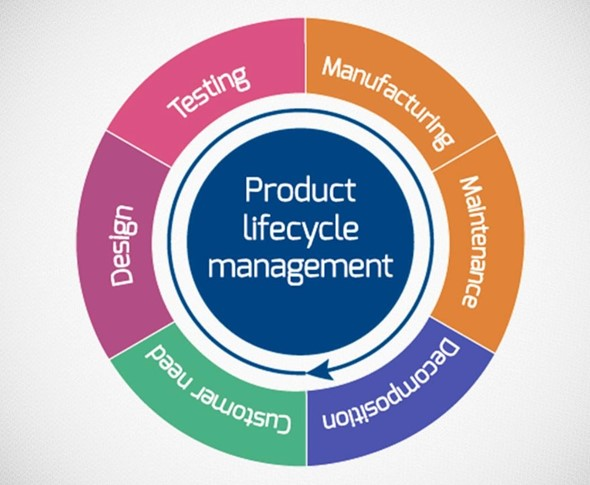
\includegraphics[width=15cm]{1}
\caption{\Large Product lifecycle stages產品生命週期階段}\label{fig.1}
\end{center}
\end{figure}
\newpage
\fontsize{14pt}{2.5pt}\sectionef 
{PLM is above all a connecting technology, not an individual technology islet or information processing system (Saaksvuori and Immonen, 2008). The idea is that every information produced by company personnel holds value equivalent to the time and money invested. Using that information saves money, not using that information wastes money. This is easier to understand when looking to a design process.}\\[1pt]

\fontsize{14pt}{5pt}\sectionef
 {PLM 首先是一種連結技術,而不是一個單獨的技術島或資訊處理系統(Saaksvuori 和 Immonen,2008)。 我們的想法是,公司人員產生的每個訊息都具有與投入的時間和金錢相當的價值。 使用該資訊可以節省金錢,而不使用該資訊會浪費金錢。 當查看設計過程時,這一點更容易理解。}\\[15pt]

\fontsize{14pt}{2.5pt}\sectionef 
{E.g. if an engineer designs an electronic circuit, the file holding the CAD drawing has an equivalent value to the time and money invested in it. The problem comes from the fact that in a traditional system only the engineer knows the design process behind the file, the extent of what is inside and its possible uses. While, from the perspective of the rest of the company, that is just a file in the database alongside thousands of others. The result is that, on its own, the information is of limited }\\[1pt]

\fontsize{14pt}{5pt}\sectionef
 {例如。 如果工程師設計電子電路,保存 CAD 圖紙的文件與投入的時間和金錢具有相同的價值。 問題在於,在傳統系統中,只有工程師知道文件背後的設計過程、內部內容的範圍及其可能的用途。 然而,從公司其他部門的角度來看,這只是資料庫中的一個文件,與數千個其他文件一起。 結果是,這些資訊本身的用途有限。}\\[15pt]

\fontsize{14pt}{2.5pt}\sectionef 
{If by any chance there is another engineer working in a similar design it will become extremely difficult for him/her to find that file and use it in his own design. Ultimately this results in waste because Engineer2 will have to spend more time and money doing something that wasalready made just because that information was not easily available or well organized. }\\[1pt]

\fontsize{14pt}{5pt}\sectionef
 {如果萬一有另一位工程師從事類似的設計,他/她將很難找到該文件並在自己的設計中使用它。 最終這會導致浪費,因為第二位工程師將不得不花費更多的時間和金錢來做一些已經完成的事情,因為這些資訊不容易獲得或組織良好。}\\[15pt]


\fontsize{14pt}{2.5pt}\sectionef 
{This scenario is not limited to product design, but also to all aspects of the product lifecycle that produces change over time. Someone had to orchestrate how that piece will be produced , how that piece will be moved,packed , distributed and disposed of. When a problem is found or improvements are possible those changes also produce information and consume resources. If the company cannot take advantage of that existing information about all those phases of the product conception it will waste resources at every single redesign.
}\\[1pt]

\fontsize{14pt}{5pt}\sectionef
 {這種場景不僅限於產品設計,還包括隨著時間的推移而產生變化的產品生命週期的各個方面。 必須有人精心策劃如何生產該作品,如何移動、包裝、分發和處置該作品。 當發現問題或可能進行改進時,這些變更也會產生資訊並消耗資源。 如果公司不能利用有關產品構思所有這些階段的現有信息,那麼每次重新設計都會浪費資源。}\\[15pt]
\newpage

\fontsize{14pt}{2.5pt}\sectionef 
{Product Lifecycle Management consists of an information system that allows information and knowledge sharing within and betweenorganizations (Sudarsan et al., 2005) minimizing the waste by controlling and organizing those files with information that would otherwise be carried only by the human resource that produced said files. The way it accomplishes that is by virtualizing all components of the product life-cycle in the form of digital “items” in an object oriented architecture. As explained by (Saaksvuori and Immonen, 2008),an item is a systematic and standard way to identify, encode and name a product, a product element or module, a component, a material or a service.
}\\[1pt]

\fontsize{14pt}{5pt}\sectionef
 {產品生命週期管理由一個資訊系統組成,該系統允許組織內部和組織之間共享資訊和知識(Sudarsan et al., 2005),透過控制和組織這些文件的資訊來最大限度地減少浪費,否則這些文件只能由產生所述文件的人力資源攜帶。 它實現這一目標的方式是在物件導向的架構中以數位「專案」的形式虛擬化產品生命週期的所有元件。 如(Saaksvuori 和 Immonen,2008)所解釋的,項目是識別、編碼和命名產品、產品元素或模組、組件、材料或服務的系統和標準方法。}\\[15pt]


\fontsize{14pt}{2.5pt}\sectionef 
{These item objects are, by all means, virtual representations that hold metadata regarding what it tries to represent and allows to connect and link the information. As described by (D’Antonio et al., 2015) product information should be connected to its production process. PLM allows to link defined processes to the product and to provide constraints on the order of process execution. E.g. a CAD drawing for a circuit schematic is attached to a virtual circuit object that holds basic information about what is contained in the file and all the previous iterations of that file over time as well as links to items representing which bill of materials (BOM) it belongs to, the machines necessary to manufacture it, the processes necessary to assemble it and more importantly how all those items changed over each improving iteration.
}\\[1pt]

\fontsize{14pt}{5pt}\sectionef
 {無論如何,這些項目物件都是虛擬表示,它們保存有關其試圖表示的內容的元數據,並允許連接和連結資訊。 如(D’Antonio 等人,2015)所述,產品資訊應與其生產過程相關聯。 PLM 允許將定義的流程連結到產品,並對流程執行的順序提供約束。 例如。 電路原理圖的 CAD 繪圖附加到虛擬電路對象,該對象保存有關文件中包含的內容以及該文件隨時間推移的所有先前迭代的基本信息,以及表示其物料清單 (BOM) 的項目的鏈接屬於,製造它所需的機器,組裝它所需的流程,更重要的是所有這些項目在每次改進迭代中如何變化。}\\[15pt]

\fontsize{14pt}{2.5pt}\sectionef 
{This all-around virtualization gives precious context to information otherwise lost on its own complexity. It allows for faster access, easier understanding of the whole and the consequences of what happens when there is change for each part. This is the best way of organizing the existing data for future reference because it allows for structure as well as transparency.
}\\[1pt]

\fontsize{14pt}{5pt}\sectionef
 {這種全方位的虛擬化為資訊提供了寶貴的背景信息,否則會因其自身的複雜性而丟失。 它允許更快地訪問、更容易理解整體以及每個部分發生變化時所發生的後果。 這是組織現有資料以供將來參考的最佳方式,因為它允許結構和透明度。}\\[15pt]
\newpage

\fontsize{14pt}{2.5pt}\sectionef 
{To sum up, PLM as a system aims to track functional change in all aspects regarding the product life, in a way that the company can benefit strategically from it by avoiding informational waste. It does so by virtualizing the real thing in the form of digital items that store the files regarding what the item is supposed to represent. These can in turn be correlated and tracked over time using metadata.
}\\[1pt]

\fontsize{14pt}{5pt}\sectionef
 {總而言之,PLM 作為一個系統,旨在追蹤產品生命週期各個方面的功能變化,從而使公司能夠透過避免資訊浪費來策略性地從中受益。 它透過以數位項目的形式虛擬化真實事物來實現這一點,這些項目儲存有關該項目應該代表的內容的文件。 這些又可以使用元資料隨著時間的推移進行關聯和追蹤。}\\[15pt]
\section{Enterprise Resource Planing 企業資源規劃}

\fontsize{14pt}{2.5pt}\sectionef 
{In the early days of information systems, one of the first systems to find wide implementation was the called MRP (Material Requirements Planning). Although not necessarily software based, this system wide implementation was a natural consequence of computing technology and it aimed to solve bottlenecks regarding the material supplying and product output by calculating the material needs for production. As it became more ubiquitous in the enterprise in the late 70’s and early 80’s the system evolved. This gave origin to MRP II (Manufacturing Resource Planning) and, more important to the scope of this paper, ERP (Enterprise Resource Planning).}

\fontsize{14pt}{5pt}\sectionef
 {在資訊系統的早期,最早被廣泛實施的系統之一是 MRP(物料需求計劃)。 儘管不一定基於軟體,但這種系統範圍的實施是計算技術的自然結果,旨在透過計算生產的材料需求來解決材料供應和產品輸出的瓶頸。 20 世紀 70 年代末和 80 年代初,隨著它在企業中變得越來越普遍,該系統也在不斷發展。 這催生了 MRP II(製造資源計劃),以及對本文範圍更重要的 ERP(企業資源計劃)。}\\[15pt]

\fontsize{14pt}{2.5pt}\sectionef 
{For the most part modern Enterprise Resource Planning expands the original MRP function to encompass many other aspects of enterprise operations all while adding modularity to the system. }

\fontsize{14pt}{5pt}\sectionef
 {現代企業資源規劃在很大程度上擴展了原始 MRP 功能,以涵蓋企業營運的許多其他方面,同時為系統添加了模組化功能。}\\[15pt]

\fontsize{14pt}{2.5pt}\sectionef 
{Modern ERP systems are often module based; different modules have different user interfaces and different user groups. For example, Manufacturing module, Procurement module, Logistics module, Financial module, Maintenance module, Sales module. (Saaksvuori and Immonen, 2008). These modules expand across many domains of knowledge but for the most part they do so always from the perspective of Production, Sales and Service. Figure 2 depicts the scope of the ERP system in comparison to other Information systems. }

\fontsize{14pt}{5pt}\sectionef
 {現代 ERP 系統通常是基於模組的; 不同的模組有不同的使用者介面和不同的使用者群組。 例如,製造模組、採購模組、物流模組、財務模組、維護模組、銷售模組。 (Saaksvuori 和 Immonen,2008)。 這些模組涵蓋了許多知識領域,但大多數情況下,它們總是從生產、銷售和服務的角度進行。 圖 2 描述了 ERP 系統與其他資訊系統相比的範圍。}\\[15pt]
\newpage
\begin{figure}[hbt!]
\begin{center}
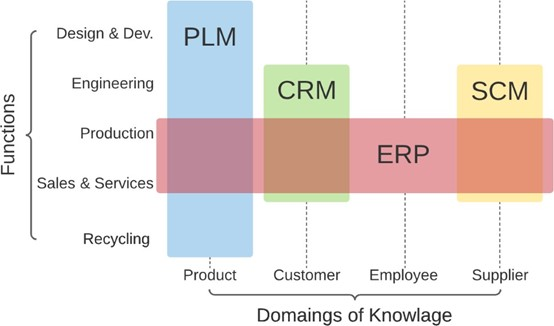
\includegraphics[width=15cm]{2}
\caption{\large Visual representation of the scope of different information systems不同資訊系統範圍的可視化表示}\label{fig.2}
\end{center}
\end{figure}

\fontsize{14pt}{2.5pt}\sectionef 
{This sort broad reach across the domains makes sense because the ERP operations, as were in the case of MRP, focus on handling transactions and orders. The focus of the ERP is controlling the change in input, retention and output of resources to the company, be of products, raw materials or packing. }

\fontsize{14pt}{5pt}\sectionef
 {這種跨領域的廣泛影響是有意義的,因為 ERP 操作與 MRP 一樣,專注於處理交易和訂單。 ERP 的重點在於控制公司資源(產品、原料或包裝)的輸入、保留和輸出的變化。}\\[15pt]

\fontsize{14pt}{2.5pt}\sectionef 
{From the same image, it is possible to see the theoretical contrast between PLM and ERP even though they are both extremely broad. While ERP expands across the domains of knowledge but limits itself to a few functions, PLM expands across all functions that involve the product. As portrayed by Figure 3, another point of view that represents a good difference between the two is the lack of overlap in what concerns the scale or level of detail in which ERP and PLM affects the industry (i.e. the granularity of the two systems).}

\fontsize{14pt}{5pt}\sectionef
 {從同一張圖中,可以看出 PLM 和 ERP 之間的理論差異,儘管它們的範圍都非常廣泛。 ERP 擴展了知識領域,但僅限於少數功能,而 PLM 擴展了涉及產品的所有功能。 如圖 3 所示,代表兩者之間良好差異的另一個觀點是 ERP 和 PLM 影響行業的規模或詳細程度(即兩個系統的粒度)方面缺乏重疊。}\\[15pt]
\newpage

\begin{figure}[hbt!]
\begin{center}
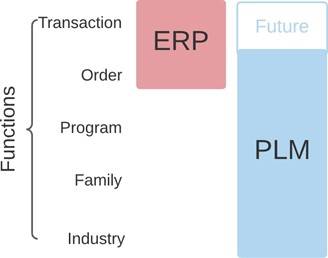
\includegraphics[width=15cm]{3}
\caption{\large Visual comparison of ERP and PLM concerning granularity ERP 和 PLM 在粒度方面的直觀比較}\label{fig.3}
\end{center}
\end{figure}

\fontsize{14pt}{2.5pt}\sectionef 
{As we can see, ERP is primarily concerned with the transaction and the order. Once an order is closed out, the ERP system processes the transactions with respect to that order but is not very much concerned with the order beyond that. On the other hand, PLM’s granularity is concerned with the order for the product and extends not only into the program, but into 
the family and the entire industry .}

\fontsize{14pt}{5pt}\sectionef
 {正如我們所看到的,ERP 主要關注的是交易和訂單。 一旦訂單關閉,ERP 系統就會處理與該訂單相關的交易,但不太關心除此之外的訂單。 另一方面,PLM 的粒度涉及產品的訂單,不僅擴展到程序,還擴展到
家庭和整個行業。}\\[15pt]
\newpage
\fontsize{14pt}{2.5pt}\sectionef 
{This is particularly interesting because it demonstrates how the two systems can and do complement each other in the field. One of the aspects of ERP that should point out is that it is comparatively easier to integrate with other systems. ERP-MES integration for instance has been widely studied and implemented to the point where standards have been developed for it (ISA 95 - IEC 62264). One argument for this is the modular nature of the ERP system which is discussed further in the paper in (Chapter 5) with the analysis of the Odoo software. That is because the Odoo software evolved originally from an open-source ERP system.}

\fontsize{14pt}{5pt}\sectionef
 {這是特別有趣的,因為它展示了這兩個系統如何能夠並且確實在該領域中相互補充。 ERP值得指出的一方面是它與其他系統的整合相對容易。 例如,ERP-MES 整合已被廣泛研究和實施,並已為其製定了標準(ISA 95 - IEC 62264)。 對此的一個論點是 ERP 系統的模組化性質,這將在本文(第 5 章)中透過對 Odoo 軟體的分析進行進一步討論。 這是因為 Odoo 軟體最初是從開源 ERP 系統發展而來的。}\\[15pt]

\fontsize{14pt}{2.5pt}\sectionef 
{The nature of the ERP system is best summed up by (Umble et al. 2003): ERP provides a unified enterprise view of the business which encompasses all functions and departments, and an enterprise database in which all actions concerning finance, sales, marketing, purchasing and human resources are traced. The aim of this achieving is to expand the customers target and increase customers share in a market that slowly pivots to innovation .
}

\fontsize{14pt}{5pt}\sectionef
 {ERP 系統的本質可以這樣概括(Umble et al. 2003):ERP 提供了一個統一的企業業務視圖,其中包含所有職能和部門,以及一個企業資料庫,其中涉及財務、銷售、行銷、採購和人力資源都被追蹤。 實現這一目標的目的是擴大客戶目標並增加緩慢轉向創新的市場中的客戶份額。}\\[15pt]
\section{Manufacturing Execution System 製造執行系統}


\fontsize{14pt}{2.5pt}\sectionef 
{The final key of a fully integrated system would be the Manufacturing Execution System (MES). A MES is a layer of communication between  he management and the production levels; it is a software that allows data exchange between the organizational level, usually supported by an ERP, and the shop-floor control systems, in which several, different, very customized software applications are employed (Meyer et al., 2009).}

\fontsize{14pt}{5pt}\sectionef
 {完全整合系統的最後一個關鍵是製造執行系統(MES)。 MES 是管理階層與生產層之間的溝通層; 它是一種允許組織層面(通常由 ERP 支援)和車間控制系統之間進行資料交換的軟體,其中使用了多種不同的、高度客製化的軟體應用程式(Meyer 等人,2009 年)。}\\[15pt]

\fontsize{14pt}{2.5pt}\sectionef 
{Figure 4 is a nice depiction of how different systems fit within the scope of manufacturing and development.}

\fontsize{14pt}{5pt}\sectionef
 {圖 4 很好地描述了不同的系統如何適應製造和開發的範圍。}\\[15pt]
\newpage

\begin{figure}[hbt!]
\begin{center}
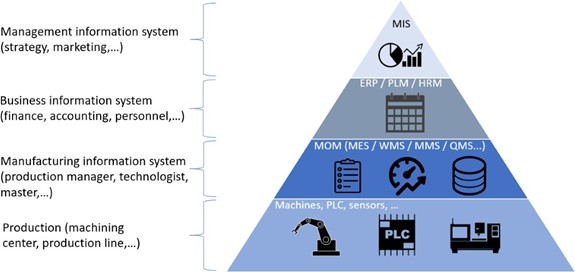
\includegraphics[width=15cm]{4}
\caption{\small Visual representation of the roll of different systems including MES\\
 包括 MES 在內的不同系統的滾動視覺化表示}\label{fig.4}
\end{center}
\end{figure}

\fontsize{14pt}{2.5pt}\sectionef 
{For all purposes MES main goal is to provide the numbers and data that ultimately is used to ascertain the condition and quality of not only the products but also all the processes that affect production. Machines, sensors, and anything that comes in contact with the product and provides output of any kind, basically, handing said data to the MES for sorting and processing in real time. E.g. if a manager wants to know the instant production numbers or to see a graphical representation of the rejection rate, that data will be available from a MES software.}

\fontsize{14pt}{5pt}\sectionef
 {出於所有目的,MES 的主要目標是提供最終用於確定產品以及影響生產的所有流程的狀況和品質的數字和數據。 機器、感測器以及與產品接觸並提供任何類型輸出的任何東西,基本上將所述資料傳遞給 MES 進行即時分類和處理。 例如。 如果經理想要了解即時生產數據或查看廢品率的圖形表示,則可以從 MES 軟體取得該數據。}\\[15pt]

\fontsize{14pt}{2.5pt}\sectionef 
{Traditionally it is from this sort of information that management will evaluate efforts and make decisions. As mentioned before this sort of data collection fits perfectly to the use of ERP not only because the management of resources can be much more detailed if complemented by real time production data but also because the modularity of ERP usually means a seamless integration. MES (like ERP) has also been proven and implemented for decades and their implementation have already been standardized to a reasonable degree.
}

\fontsize{14pt}{5pt}\sectionef
 {傳統上,管理層將根據此類資訊評估工作並做出決策。 如前所述,這種數據收集非常適合 ERP 的使用,不僅因為如果輔以即時生產數據,資源管理可以更加詳細,而且還因為 ERP 的模組化通常意味著無縫整合。 MES(如 ERP)也已被證明和實施了數十年,其實施已達到合理的標準化程度。}\\[15pt]
\newpage



\fontsize{14pt}{2.5pt}\sectionef 
{The functionalities of a MES have been grouped in 11 categories by MESA International(1997); furthermore, the tasks for each enterprise layer and, in turn, for each kind of information system are listed in the ISA95 – IEC62264 (2013) standard. This standard also provides definitions for the data structures to be exchanged among information systems aiming to enhance their integration; however, it mainly focuses on ERP-MES-Shop floor integration (D’Antonio et al., 2015).
}

\fontsize{14pt}{5pt}\sectionef
 {MESA International (1997) 將 MES 的功能分為 11 類; 此外,ISA95 – IEC62264 (2013) 標準中列出了每個企業層以及每種資訊系統的任務。 該標準還提供了資訊系統之間交換的資料結構的定義,旨在增強資訊系統的整合度; 然而,它主要關注 ERP-MES-車間整合(D’Antonio 等,2015)。}\\[15pt]


\fontsize{14pt}{2.5pt}\sectionef 
{PLM studies by comparison are much more recent and PLM-MES integration, a main focus of this work, even more so. The challenge of this sort of integration and the state of the art regarding it was be covered in (Chapter 3) as well as the theoretical structure behind it. For now, suffice to point out that since MES provides the feedback by which changes are orchestrated and results are validated by generating information in the form of files and PLM focus on the tracking change by file organization there sure is value in the PLM-MES 

}

\fontsize{14pt}{5pt}\sectionef
 {相較之下,PLM 研究是較新的,而 PLM-MES 整合(這項工作的主要焦點)更是如此。 (第 3 章)及其背後的理論結構涵蓋了這種整合的挑戰和相關的最新技術。 目前,只需指出,由於 MES 提供回饋,透過產生文件形式的資訊來編排變更並驗證結果,而 PLM 專注於按文件組織追蹤變更,因此 PLM-MES 確實有價值
一體化。}\\[15pt]

\section{Industry 4.0 工業4.0}

\fontsize{14pt}{2.5pt}\sectionef 
{The term Industry 4.0 is one mentioned time and time again in modern literature as the next or current step in the evolution of production. It represents what is the 4th industrial revolution where the first was marked the adoption of steam power, the second was marked mainly using electrical power and the 3rd was characterized by the implementation of digital technology. Figure 5 nicely represents the progression of industrial revolutions.


}

\fontsize{14pt}{5pt}\sectionef
 {工業 4.0 一詞在現代文獻中被多次提及,被視為生產演變的下一步或當前步驟。 它代表了第四次工業革命,第一次工業革命的特徵是蒸汽動力的採用,第二次工業革命的特徵是主要使用電力,第三次工業革命的特徵是數位技術的實施。 圖 5 很好地展示了工業革命的進展。}\\[15pt]
\newpage
\begin{figure}[hbt!]
\begin{center}
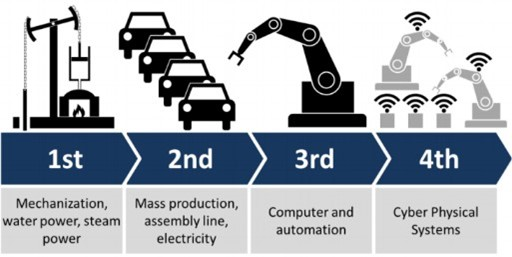
\includegraphics[width=15cm]{5}
\caption{\large The industry evolution產業演變}\label{fig.5}
\end{center}
\end{figure}


\fontsize{14pt}{2.5pt}\sectionef 
{In broad strokes the 4th industrial revolution is (or will be) ultimately marked by the full integration between digital connectivity and production. As it is well known that the development of digital networks is the pivotal technology that sustain the modern world. It has changed the way humans interact and do business. However, whether the current level in which it is applied to the industry constitutes an industrial revolution is still uncertain because in all other revolutions have been marked by a violent increase in production that is yet to happen this time around. In fact, we are still to reach a shared definition of Industry 4.0.
}

\fontsize{14pt}{5pt}\sectionef
 {從廣義上講,第四次工業革命的最終標誌是(或將)數位連接與生產之間的全面整合。 眾所周知,數位網路的發展是維持現代世界的關鍵技術。 它改變了人類互動和開展業務的方式。 然而,目前它應用於工業的水平是否構成工業革命仍然不確定,因為在所有其他革命中,其標誌都是產量的劇烈增加,而這一次尚未發生。 事實上,我們仍然沒有對工業4.0達成共同的定義。}\\[15pt]

\fontsize{14pt}{2.5pt}\sectionef 
{What has been widely accepted however is that there are at least 3 technologies that characterize Industry 4.0. Those are the Internet of things (IoT), Cloud computing and the development of Cyber-Physical Systems (CPS), the last of which is particularly important for the context of this thesis.}

\fontsize{14pt}{5pt}\sectionef
 {然而,人們普遍認為至少有 3 種技術可以表徵工業 4.0。 這些是物聯網(IoT)、雲端運算和網路物理系統(CPS)的發展,最後一個對於本論文的背景尤其重要。}\\[15pt]

\newpage



\fontsize{14pt}{2.5pt}\sectionef 
{CPS are systems consisting in a real entity (for example, a machine) and its corresponding virtual model – embedding all the models for mimicking the behavior of the real counterpart – capable to communicate with each other (D’Antonio et al., 2017). The idea is that, if one were to develop a digital twin (DT) of all physical instruments regarding a process in a system that allows for the digital counterparts to interact with each other as well as interacting with the physical world, innovation or change of said process would occur much faster and effectively. E.g., an engineer could simulate a change using the DT’s interaction, then, if successful, apply the change automatically to the production line in real time, execute tests, gather data and feed it back to the system without the need of manual input with all being done through the network.}

\fontsize{14pt}{5pt}\sectionef
 {CPS 是由真實實體(例如機器)及其相應的虛擬模型組成的系統 - 嵌入所有用於模仿真實對應物行為的模型 - 能夠相互通信(D'Antonio 等人,2017) 。 這個想法是,如果要開發所有實體儀器的數位孿生(DT),涉及系統中的一個過程,允許數位對應物相互交互以及與物理世界交互,創新或改變該過程將發生得更快、更有效。 例如,工程師可以使用DT的交互來模擬變更,然後,如果成功,則將變更自動即時應用到生產線,執行測試,收集數據並將其反饋給系統,而無需手動輸入所有內容是透過網路完成的。}\\[15pt]

\fontsize{14pt}{2.5pt}\sectionef 
{The main point to be derived from all this is that PLM-MES systems possibly are the first step to achieve a proper CPS since it provides for the virtualization and necessary control to reach something near a virtual twin. The debatable matter is how deep is its current effect in industrial application.}

\fontsize{14pt}{5pt}\sectionef
 {從這一切中得出的要點是,PLM-MES 系統可能是實現適當 CPS 的第一步,因為它提供了虛擬化和必要的控制來達到接近虛擬孿生的效果。 值得爭議的問題是它目前在工業應用中的影響有多深。}\\[15pt]

\fontsize{14pt}{2.5pt}\sectionef 
{Nonetheless, the term Industry 4.0 is, if anything, a useful denotation to the increasing application of digital connectivity, network development and the internet to industry.}

\fontsize{14pt}{5pt}\sectionef
 {儘管如此,工業 4.0 這個術語如果有的話,也是對數位連接、網路發展和互聯網在工業中日益增長的應用的有用表示。}\\[15pt]

\fontsize{14pt}{2.5pt}\sectionef 
{Another term often included within the scope of Industry 4.0 is the called Lot Size One or Lot 1. This is the idea of each item customized to the individual specifications of the buyer in a system in which a customer order does not start supply chain equipment moving; it turns on manufacturing machines.}

\fontsize{14pt}{5pt}\sectionef
 {工業4.0 範圍內經常包含的另一個術語稱為“批量大小一”或“批量1”。這是在系統中根據買方的個人規格定制每個項目的想法,在該系統中,客戶訂單不會啟動供應鏈設備移動; 它打開製造機器。}\\[15pt]
\newpage

\fontsize{14pt}{2.5pt}\sectionef 
{The theory behind it is that as production and development becomes more and more flexible as this sort of manufacturing becomes not only viable but also attractive. Having a tailored requested product means that there are no storage requirements, no inventory overhead, and of course a 100percent guaranteed sell. This concept is not new by any means, in fact it predates Industry 4.0 quite a lot. In the book “The machine that changed the world”the authors (Womack et al., 1990) discuss that toward this end, lean producers employ teams of multiskilled workers at all levels of the organization and use highly flexible, increasingly automated machines to produce volumes of products in enormous variety.}

\fontsize{14pt}{5pt}\sectionef
 {背後的理論是,隨著生產和開發變得越來越靈活,這種製造不僅變得可行而且有吸引力。 擁有量身訂製的需求產品意味著沒有儲存要求、沒有庫存開銷,當然還有 100percent 的銷售保證。 無論如何,這個概念並不新鮮,事實上它早在工業 4.0 之前就出現了。 在《改變世界的機器》一書中,作者(Womack 等人,1990)討論了為此目的,精益生產者在組織的各個層面僱用多技能工人團隊,並使用高度靈活、自動化程度越來越高的機器來生產大量種類繁多的產品。}\\[15pt]

\fontsize{14pt}{2.5pt}\sectionef 
{In a way ‘Lot Size One’ is nothing more than the extrapolation of this sort of thinking. Of course, the industry is yet to reach such level of production flexibility, but glimpses of this sort of mentality can already be seem on more modular productions. One of the best examples is amazon packing systems. E.g. a customer receives a package from Amazon containing a mix of products that has been packaged just for him/her according to their specific order. Although superficial in nature, this represents a high level of customization for the customer. }

\fontsize{14pt}{5pt}\sectionef
 {在某種程度上,「批量一」只不過是這種思考的推論。 當然,該行業尚未達到這樣的生產靈活性水平,但這種心態已經可以在更模組化的生產中看到。 最好的例子之一是亞馬遜包裝系統。 例如。 客戶收到亞馬遜的包裹,其中包含根據其特定訂單專門為他/她包裝的產品組合。 雖然本質上很膚淺,但這代表了客戶的高水準客製化。}\\[15pt]

\fontsize{14pt}{2.5pt}\sectionef 
{Another great example is electronics prototyping. Currently there are companies that take your printed circuit board designs and BOM, delivering small batches of assembled prototypes at a low cost. Prototyping of electronical devices used to be a highly expensive process, but some companies have flexibilized their production to the degree where they are able to deliver it fast and reliably. Again, that is possible because electronics components are inherently modular systems even if of high complexity. The following image (Figure 6 Example project of power supply adaptor circuit) is an example of an electronic circuit that was designed by this student and manufactured by JLCPCB within a single week.}

\fontsize{14pt}{5pt}\sectionef
 {另一個很好的例子是電子原型設計。 目前,有些公司會採用您的印刷電路板設計和 BOM,以低成本提供小批量的組裝原型。 電子設備的原型設計曾經是一個非常昂貴的過程,但一些公司已經將其生產靈活化到能夠快速可靠地交付的程度。 同樣,這是可能的,因為電子元件本質上是模組化系統,即使其複雜性很高。 下圖(圖6電源適配器電路範例專案)是該學生設計並由JLCPCB在一週內製造的電子電路範例。}\\[15pt]
\newpage

\begin{figure}[hbt!]
\begin{center}
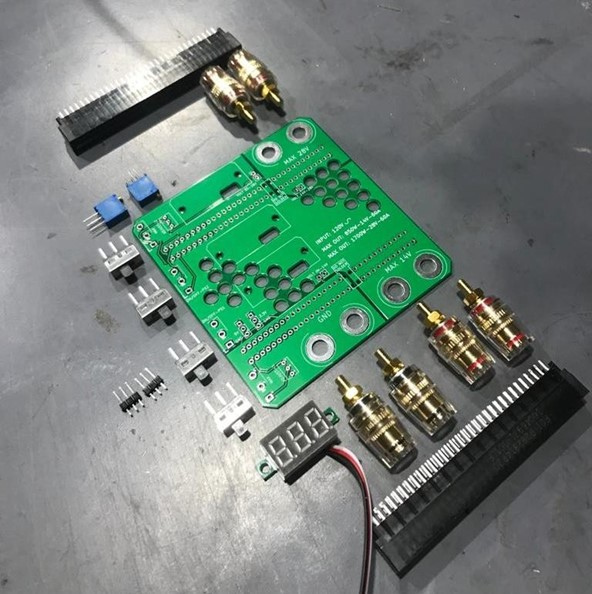
\includegraphics[width=15cm]{6}
\caption{\large Example project of power supply adaptor circuit\\電源適配器電路範例項目}\label{fig.6}
\end{center}
\end{figure}

\fontsize{14pt}{2.5pt}\sectionef 
{All and all, the result is again a greater need for control and management of change. Which means the implementation of a PLM-MES system would be of great help. PLM would be required to manage change and innovation throughout the lifecycle of small batch products and MES would provide the real time reaction and feedback necessary to reduce errors that could cause losing a whole batch.
}

\fontsize{14pt}{5pt}\sectionef
 {總而言之,結果再次是對變革的控制和管理的更大需求。 這意味著PLM-MES系統的實施將會有很大的幫助。 PLM 需要在小批量產品的整個生命週期中管理變更和創新,而 MES 將提供必要的即時反應和回饋,以減少可能導致整批產品遺失的錯誤。}\\[15pt]
\newpage
\chapter{THE STATE OF THE ART AND THE INTEGRATION OF PLM AND MES} 
\pagenumbering{arabic} %設定頁號阿拉伯數字
\setcounter{page}{17}  %設定頁數
\begin{center}
\fontsize{18}{16}\selectfont \textbf{最先進的技術以及 PLM 和 MES 的集成}\\
\end{center}
\vspace{2em}

\fontsize{14pt}{2.5pt}\sectionef 
{Unfortunately, there are not many published studies in the matter of integration between PLM and MES systems. But there seems to be a consensus in the most probable effects of said integration. Those being synchronization and tighter tolerances.}\\[10pt]

\fontsize{14pt}{5pt}\sectionef
 {遺憾的是,關於 PLM 和 MES 系統整合問題的已發表研究並不多。但對於上述整合最可能產生的影響似乎已達成共識。這些是同步和更嚴格的公差。}\\[15pt]

\fontsize{14pt}{2.5pt}\sectionef 
{As explained by D’Antonio et al. (2015), which focus on a case study involving the manufacturing of precision components for aeronautical applications, the first advantage expected by the deployment of the monitoring and control system is product quality improvement: sensors allow to detect, measure and monitor variables, events and situations that affect process performance or product quality.}\\[10pt]

\fontsize{14pt}{5pt}\sectionef
 {正如德安東尼奧等人所解釋的。 (2015),重點在於涉及航空應用精密零件製造的案例研究,部署監控系統預期的第一個優勢是產品品質改進:感測器允許檢測、測量和監控變數、事件和影響製程性能或產品品質的情況。
}\\[15pt]

\fontsize{14pt}{2.5pt}\sectionef 
{One of the central problems regarding integrating PLM with any other system revolves around the ownership of information. A possible solution relies on database integration as well as the use of middleware between systems. As is written in Saaksvuori and Immonen, (2008). A reasonable objective is that information should always be updated in one place. Other systems can read information directly from the PLM databases, and if necessary, the required information can be replicated on the databases of other system, as depicted in Figure7. Although it points this out mainly from the perspective of PLM-ERP integration, it is still very valuable from the perspective of PLM-MES integration because it is an example of how the better operation can be expected by working around systems in which files of different nature are loaded into a centralized PLM-ERP system.}\\[10pt]

\fontsize{14pt}{5pt}\sectionef
 {將 PLM 與任何其他系統整合的核心問題之一涉及資訊的所有權。一種可能的解決方案依賴於資料庫整合以及系統之間中間件的使用。正如 Saaksvuori 和 Immonen (2008) 所寫。一個合理的目標是資訊應始終在一個地方更新。其他系統可以直接從PLM資料庫中讀取訊息,如果需要,可以將所需資訊複製到其他系統的資料庫上,如圖7所示。雖然主要是從PLM-ERP整合的角度指出了這一點,但從PLM-MES 整合的角度來看,仍然非常有價值,因為它是一個範例,說明如何透過將不同性質的檔案載入到集中式PLM-ERP 系統中的系統來實現更好的操作。
}\\[15pt]
\begin{figure}[hbt!]
\begin{center}
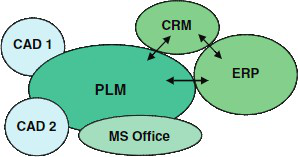
\includegraphics[width=10cm]{7}
\caption{\Large Diagram of PLM integration PLM整合示意圖}\label{fig.7}
\end{center}
\end{figure}

\fontsize{14pt}{2.5pt}\sectionef 
{The middleware would therefore be a software framework to organize and connect all the information given to the system database in a user-friendly way. This sort of application is also referred to as integration application and, as specified by Stark (2015), these applications enable exchange of product information between PLM applications (for example, between a CAD application and a CAE application). They also enable exchange of product information between PLM applications and other enterprise applications such as ERP and CRM.}\\[10pt]

\fontsize{14pt}{5pt}\sectionef
 {因此,中間件將成為一個軟體框架,以使用者友好的方式組織和連接提供給系統資料庫的所有資訊。此類應用程式也稱為整合應用程序,並且根據 Stark (2015) 的規定,這些應用程式支援在 PLM 應用程式之間(例如 CAD 應用程式和 CAE 應用程式之間)交換產品資訊。它們還支援 PLM 應用程式與其他企業應用程式(例如 ERP 和 CRM)之間的產品資訊交換。}\\[15pt]

\fontsize{14pt}{2.5pt}\sectionef 
{In a very relevant fashion, this middleware line of thinking is expanded upon by (Ben Khedher et al., 2011). In their work regarding different systems architectures for the implementation of an integrated MES+PLM they describe the use of a mediation system in web service architecture. As depicted in Figure 8, the proposed architecture uses data exchange based on internet technologies to help companies, especially expanded companies, to take advantage of opportunities generated by the Web Services. The concept of "web service" means an application (program or software system) which is designed to support interoperable machine-to-machine interactions over a network, according to the definition of W3C (Ben Khedher et al., 2011).}\\[10pt]

\fontsize{14pt}{5pt}\sectionef
 {(Ben Khedher et al., 2011) 以非常相關的方式擴展了這種中間件思路。在他們關於實施整合 MES+PLM 的不同系統架構的工作中,他們描述了中介系統在 Web 服務架構中的使用。如圖 8 所示,所提出的架構使用基於互聯網技術的資料交換來幫助公司,特別是擴張型公司,利用 Web 服務產生的機會。根據 W3C 的定義,「Web 服務」的概念是指旨在支援網路上可互通的機器對機器互動的應用程式(程式或軟體系統)(Ben Khedher 等,2011)。}\\[15pt]
\newpage

\begin{figure}[hbt!]
\begin{center}
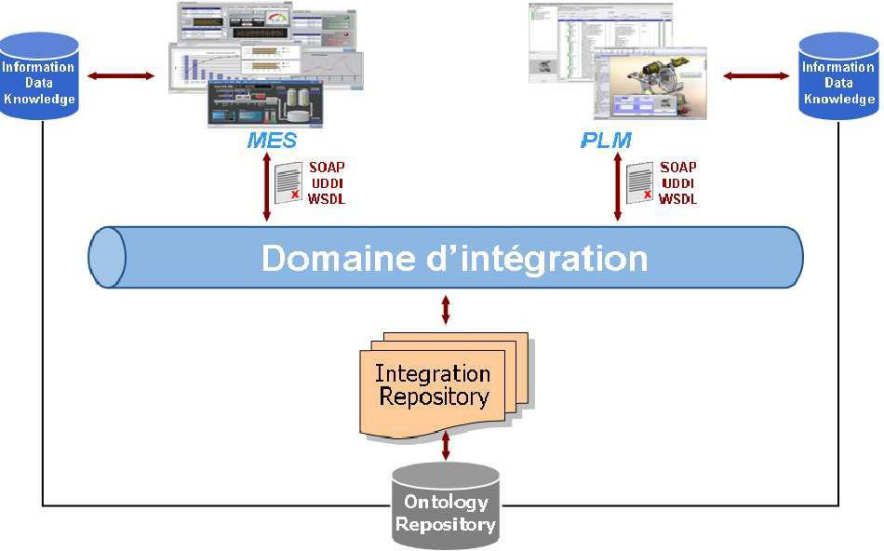
\includegraphics[width=15cm]{8}
\caption{\Large Diagram of Web service architecture Web服務架構圖}\label{fig.8}
\end{center}
\end{figure}

\fontsize{14pt}{2.5pt}\sectionef 
{The reason this expansion is so relevant from the perspective of this work is that the Odoo software works in a similar fashion through a similar web service architecture. In theory the Odoo software could act as the middleware working through the local network or hosted in the cloud and enacting the layer of integration that was previously mentioned.}\\[10pt]

\fontsize{14pt}{5pt}\sectionef
 {從這項工作的角度來看,這種擴展如此相關的原因是 Odoo 軟體透過類似的 Web 服務架構以類似的方式運作。理論上,Odoo 軟體可以充當透過本地網路工作或託管在雲端中的中間件,並執行前面提到的整合層。}\\[15pt]

\section{How would this integration look like in practical terms 這種整合在實際中會是什麼樣子}

\fontsize{14pt}{2.5pt}\sectionef 
{As mentioned in CHAPTER 2 the main idea of PLM is to manage change in all processes related to the product, and it does so mainly through the use of virtualization. The word virtualization here denotes representation of item of the real world to the digital space and, as one can imagine, there are several levels of abstraction through which a real object or process can be represented. As consequence there is no exact consensus regarding PLM of how deep and/or detailed the virtual representation must be to serve its purpose.}\\[10pt]

\fontsize{14pt}{5pt}\sectionef
 {如第 2 章中所提到的,PLM 的主要想法是管理與產品相關的所有流程中的變更,它主要透過使用虛擬化來實現。這裡的「虛擬化」一詞表示現實世界的項目在數位空間中的表示,並且正如人們可以想像的那樣,可以透過多個抽象層級來表示真實的物件或過程。因此,對於 PLM 虛擬表示必須有多深和/或多詳細才能達到其目的,還沒有達成確切的共識。}\\[15pt]

\fontsize{14pt}{2.5pt}\sectionef 
{In an ideal world that would be the lowest form of abstraction which, essentially, would come down to a digital twin as explained in the CHAPTER 2. This is a ‘1 to 1’ digital representation of every aspect of the production cycle where every part involved would have a digital representation that not only carry the physical characteristics of the item but also all its information produced over time. To this end, as explained in CHAPTER 2, MES takes a fundamental role in obtaining the real time information required for the DT even be possible.}\\[10pt]

\fontsize{14pt}{5pt}\sectionef
 {在理想的世界中,這將是最低的抽象形式,本質上將歸結為數位孿生,如第 2 章所述。這是生產週期各個方面的「1 對 1」數字表示,其中每個部分所涉及的內容將具有數位表示,不僅包含該項目的物理特徵,還包含隨著時間的推移產生的所有資訊。為此,如第 2 章所述,MES 在獲取 DT 所需的即時資訊方面發揮基礎作用,甚至是可能的。}\\[15pt]

\fontsize{14pt}{2.5pt}\sectionef 
{For instance, a CNC machine would have a digital 3D model for simulation as well as a fully integrated list of all the pieces it produces, data regarding its current level of production, the current wear of its mechanical pieces, all other machines it relates to, history of all the alterations and improvements by which it was affected and many other aspects, all well packaged in an intuitive graphical user interface (GUI) that allows for maximum interaction.}\\[10pt]

\fontsize{14pt}{5pt}\sectionef
 {例如,數控機床將具有用於模擬的數位 3D 模型以及其生產的所有零件的完全整合清單、有關其當前生產水平的數據、其機械零件的當前磨損情況以及與其相關的所有其他機器、受影響的所有變更和改進的歷史記錄以及許多其他方面,全部都很好地封裝在直覺的圖形使用者介面(GUI) 中,可實現最大程度的互動。}\\[15pt]

\fontsize{14pt}{2.5pt}\sectionef 
{Outside of fiction, we are yet to achieve such level of virtualization. It takes too much time and money to obtain and organize information to such a level of minutia, specially, the aspects that need to be inserted by hand, not to mention the subjectiveness of how this information can be integrated and interacted with. Regardless of that it is useful to identify, within the ideal, the aspects of most importance for this implementation.}\\[10pt]

\fontsize{14pt}{5pt}\sectionef
 {除了小說之外,我們還沒有達到這樣的虛擬化程度。獲取和組織如此詳細的資訊需要花費太多的時間和金錢,特別是需要手動插入的方面,更不用說如何整合和互動這些資訊的主觀性了。不管怎樣,在理想情況下確定對於此實施最重要的方面是有用的。}\\[15pt]

\fontsize{12}{2.5pt}\selectfont {Those are:}\\[1pt]
\fontsize{12}{2.5pt}\selectfont {那些是:}\\[15pt]

\begin{enumerate}[{\hspace{0.5em}\textbullet}]
\fontsize{12}{2.5pt}\selectfont
\item The means of virtualization – What sort of information is used to build the virtual items. This includes the metadata and files that are directly attached to the item. In an ideal fashion this would contain all possible information available about the item.\\
虛擬化的手段-使用什麼樣的資訊來建構虛擬物品。這包括直接附加到項目的元資料和文件。在理想的情況下,這將包含有關該項目的所有可能的可用資訊。
\item The means of data input - How this information is being loaded and organized. Ideally this information would be loaded into the system as automatically as possible, be it by means of MES during quality control or through the use of automated input tools like bar code scanners.\\
資料輸入的方式 - 如何載入和組織這些資訊。理想情況下,這些資訊將盡可能自動載入到系統中,無論是在品質控制期間透過 MES 還是透過使用條碼掃描器等自動輸入工具。
\item The means of access – How this information is presented to the users. Although more subjective than the previous aspects this is incredibly important to the way the system is interacted with. How intuitive it is the information availability plays right into the core strengths of PLM. Afterall, everything would be for nothing (even if all else would be perfect) if the only way to interact with the system were a command line interface that would make difficult for the end users to access the information.\\
存取方式-如何將資訊呈現給使用者。儘管比前面的方面更主觀,但這對於系統互動的方式非常重要。資訊可用性的直覺程度正是 PLM 的核心優勢。畢竟,如果與系統互動的唯一方式是命令列介面,而這將使最終用戶存取資訊變得困難,那麼一切都將毫無意義(即使其他一切都很完美)。
\item The means of integration - How items and their contained information can interact and benefit from one another, i.e., the integration with other systems and key softwares. E.g., if an item has access to a cad file, there should be no need to fill in the metadata fields by hand. Hoe items can automatically affect other items also plays into this aspect.\\
整合方式 - 專案及其所包含的資訊如何互動並相互受益,即與其他系統和關鍵軟體的整合。例如,如果某個項目可以存取 cad 文件,則無需手動填寫元資料欄位。鋤頭項目可以自動影響其他項目也能發揮作用。

\end{enumerate}
\renewcommand{\baselinestretch}{0.5} %設定行距
\newpage
\chapter{INTRODUCTION TO THE COMPANY AND PRODUCT} 
\pagenumbering{arabic} %設定頁號阿拉伯數字
\setcounter{page}{22}  %設定頁數
\begin{center}
\fontsize{18}{16}\selectfont \textbf{公司及產品介紹}\\
\end{center}
\vspace{1em}

\fontsize{14pt}{2.5pt}\sectionef 
{As one can imagine, one of the unique aspects of this work is its focus in one specific software solution that tend to be quite flexible in terms of ease of implementation to different sorts of business. This is contrary to most use cases regarding PLM implementation where the business case is the constant and the system is built around it. Nonetheless, in order to evaluate Odoo as a PLM+MES tool, it is important to consider an example. The advantage here is that a fictional company can be picked for this end maximizing the perceived effect of the software during a simulation.}\\[5pt]

\fontsize{14pt}{5pt}\sectionef
 {可以想像,這項工作的獨特之處之一是它專注於一個特定的軟體解決方案,該解決方案在易於實施不同類型的業務方面往往非常靈活。這與大多數有關 PLM 實施的用例相反,在這些用例中,業務案例是不變的,系統是圍繞它構建的。儘管如此,為了評估 Odoo 作為 PLM+MES 工具的能力,考慮一個範例很重要。這裡的優點是可以選擇一家虛構的公司來實現這一目的,從而在模擬過程中最大化軟體的感知效果。}\\[15pt]

\fontsize{14pt}{2.5pt}\sectionef 
{It is considering all those previously mentioned systems that, for the sake of exemplification, the theoretical company was organized in the molds of Industry 4.0. This company is a recently founded small case manufacturing company that uses plastic injection molding as their primary mean of production and uses additive manufacturing and fast prototyping as part of their business strategy. As explained in chapter 2 those are great examples of the path that industry is taking regarding innovation where mass production is becoming slowly less important than product variety and time to market.}\\[5pt]

\fontsize{14pt}{5pt}\sectionef
 {考慮到前面提到的所有系統,為了舉例說明,理論公司是按照工業 4.0 的模式組織的。該公司是一家最近成立的小型箱體製造公司,使用塑膠射出成型作為主要生產方式,並使用積層製造和快速原型製作作為其業務策略的一部分。如第 2 章所解釋的,這些都是產業在創新方面所採取的路徑的很好的例子,在這種創新中,大規模生產逐漸變得不如產品品種和上市時間重要。}\\[15pt]

\fontsize{14pt}{2.5pt}\sectionef 
{In order to maximize the tracking of change, most of its business are based on lower production batches on mainly automated machinery. This company focus in the production of injected plastic products and rely heavily in flexible machinery for setting production and prototyping. Having that in mind, it should be simple enough to simulate continuous improvement of both product and process to the extent of the evaluated software. Since this sort of everchanging production is extremely dependent on information management of all kinds, it must prove to be a perfect base for applied PLM+MES.}\\[5pt]

\fontsize{14pt}{5pt}\sectionef
 {為了最大限度地追蹤變化,其大部分業務都基於主要自動化機械上的較低生產批次。該公司專注於注射塑膠產品的生產,並嚴重依賴靈活的機械來進行生產和原型製作。考慮到這一點,它應該足夠簡單,可以在評估的軟體範圍內模擬產品和流程的持續改進。由於這種不斷變化的生產極其依賴各種資訊管理,因此它必須成為應用 PLM+MES 的完美基礎。}\\[15pt]

\fontsize{14pt}{2.5pt}\sectionef 
{In this example the company has already implemented, since its recent foundation, the Odoo software and has taken all the necessary training and steps to its proper use. This allow the removal of the boundaries and limitations that are so common regarding implementation of the PLM+MES system to an already existing business, i.e., dependences on legacy systems administrative resistance to change or integration to old procedures. These are obviously important, but it is not within the scope of this work.}\\[10pt]

\fontsize{14pt}{5pt}\sectionef
 {在這個例子中,該公司自最近成立以來已經實施了 Odoo 軟體,並採取了所有必要的培訓和步驟來正確使用該軟體。這樣可以消除在現有業務中實施 PLM+MES 系統時常見的邊界和限制,即依賴遺留系統管理對更改或整合舊程式的抵制。這些顯然很重要,但不屬於本工作的範圍。}\\[15pt]

\fontsize{14pt}{2.5pt}\sectionef 
{The company aims to produce a completely new product by the end of the year. After doing so, the company improved the process of production for said product. Once there is the need for product improvement, said improvement was performed as well.}\\[10pt]

\fontsize{14pt}{5pt}\sectionef
 {該公司的目標是在今年底前生產出全新的產品。在此之後,該公司改進了該產品的生產流程。一旦產品需要改進,也進行改進。}\\[15pt]

\fontsize{14pt}{2.5pt}\sectionef 
{The following diagram (Figure 9) will be taken into consideration as the path of product development and improvement:}\\[10pt]

\fontsize{14pt}{5pt}\sectionef
 {將考慮下圖(圖9)作為產品開發和改進的路徑:}\\[15pt]

\begin{figure}[hbt!]
\begin{center}
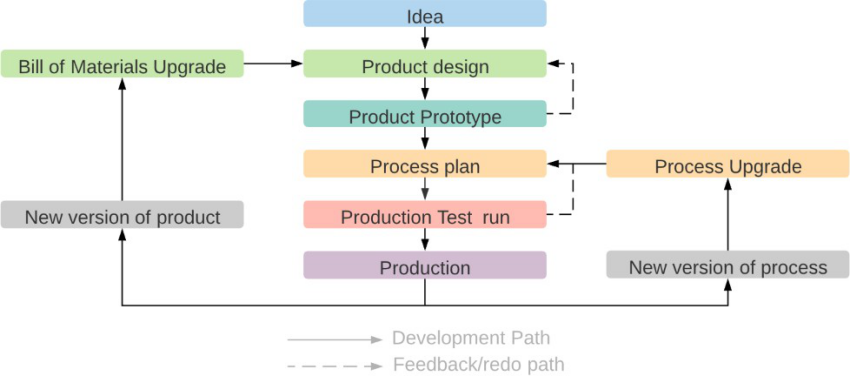
\includegraphics[width=15cm]{9}
\caption{\Large Development diagram 開發圖}\label{fig.9}
\end{center}
\end{figure}

\fontsize{14pt}{2.5pt}\sectionef 
{This path aims to transmit to the reader an iterative approach towards development and improvement. The idea is followed by a product design for which a cycle of prototyping and redesign takes effect until satisfactory result is achieved. Then a similar cycle takes place regarding the production process. At the end of this stage initial development is done and the actual production can begin.}\\[10pt]

\fontsize{14pt}{5pt}\sectionef
 {這條路徑旨在向讀者傳達一種開發和改進的迭代方法。這個想法之後是產品設計,原型製作和重新設計的循環生效,直到獲得滿意的結果。然後在生產過程中會發生類似的循環。在此階段結束時,初步開發完成,實際生產即可開始。}\\[15pt]

\fontsize{14pt}{2.5pt}\sectionef 
{It is at this point that ways of stablishing the continuous improvement is important. In the case of this company, we are only considering two main types of upgrade paths, those being, product upgrade and process upgrade respectively.}\\[10pt]

\fontsize{14pt}{5pt}\sectionef
 {正是在這一點上,建立持續改進的方法很重要。就這家公司而言,我們只考慮兩個主要的升級路徑,分別是產品升級和流程升級。}\\[15pt]

\section{The products and processes 產品和工藝}

\fontsize{14pt}{2.5pt}\sectionef 
{Change and effect are the focus of the PLM+MES implementation as such the subject of said change would ideally be something that could afford a reasonable amount of freedom of design. Although the effects of a well implemented PLM+MES should be substantial even in rigid manufacturing environments, where the change is extremely limited, the system will produce much more perceivable change in an enterprise that thrives in innovation because there will be more opportunities to improve the system and gain feedback.}\\[10pt]

\fontsize{14pt}{5pt}\sectionef
 {變更和效果是 PLM+MES 實施的重點,因此理想情況下,上述變更的主題應該能夠提供合理的設計自由。雖然實施良好的PLM+MES 的效果即使在變化極其有限的嚴格製造環境中也應該是顯著的,但該系統將在創新蓬勃發展的企業中產生更明顯的變化,因為將有更多的機會來改進系統並獲得回饋。}\\[15pt]

\fontsize{14pt}{2.5pt}\sectionef 
{From the perspective of improvement, if you compare a product that is a result from sheet metal stamping (Figure 10) to an equivalent product that is the result of a CNC milling procedure (Figure 11) it is easy to perceive that the CNC milled product is more welcoming to upgrades. While the stamping is low cost (by comparison) it depends on heavy high precision metal dyes that are extremely expensive to produce. This means that the cost of enacting change to it is much higher and thus the effect of a system that thrives on tracking change becomes limited.}\\[10pt]

\fontsize{14pt}{5pt}\sectionef
 {從改進的角度來看,如果將鈑金沖壓的產品(圖 10)與 CNC 銑削加工的同等產品(圖 11)進行比較,很容易看出 CNC 銑削的產品更歡迎升級。雖然沖壓成本較低(相比之下),但它依賴於生產成本極其昂貴的重型高精度金屬染料。這意味著對其進行更改的成本要高得多,因此依靠追蹤更改而蓬勃發展的系統的效果變得有限。}\\[15pt]
\newpage

\begin{figure}[hbt!]
\begin{center}
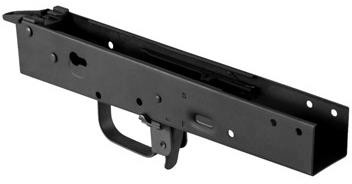
\includegraphics[width=15cm]{10}
\caption{\Large Example of stamped AK74 pattern rifle receiver (Brownnells.com) 印有AK74圖案的步槍機匣範例 (Brownnells.com)}\label{fig.10}
\end{center}
\end{figure}

\begin{figure}[hbt!]
\begin{center}
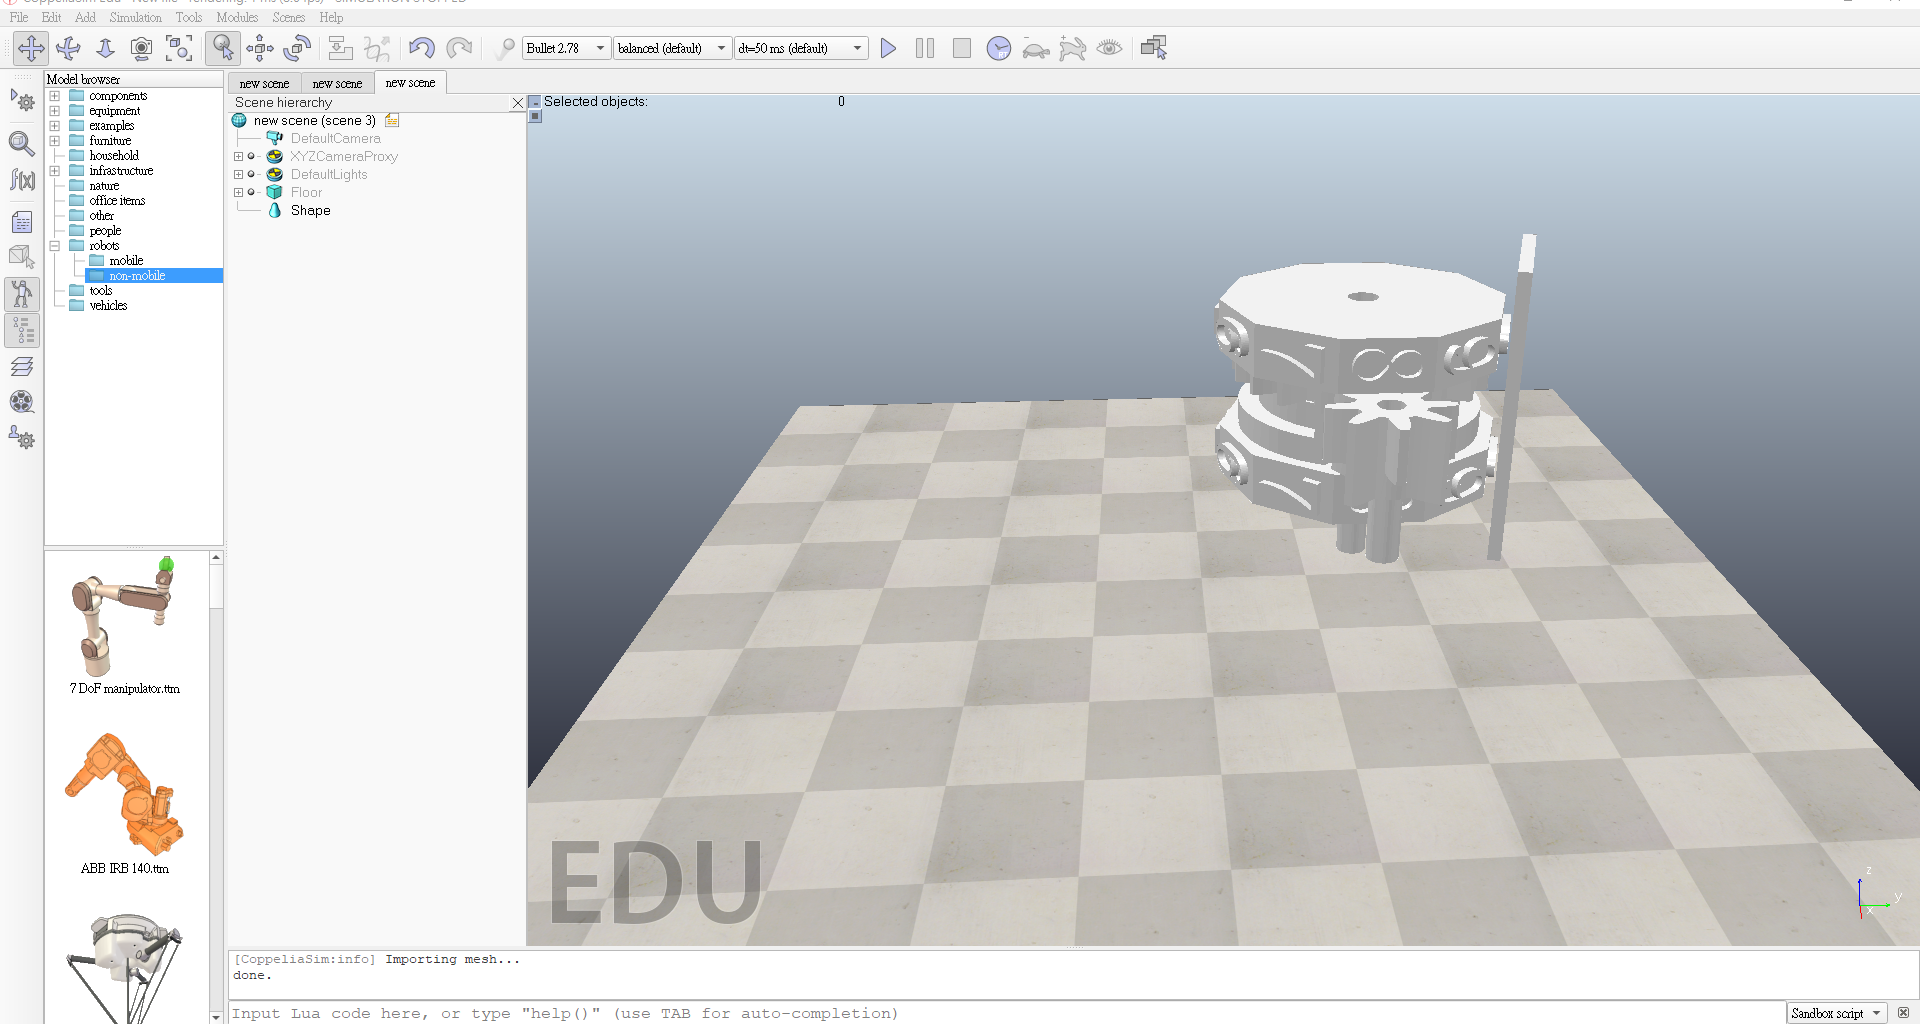
\includegraphics[width=15cm]{11}
\caption{\Large Example of milled AK74 pattern rifle receiver (sharpsbros.com) 銑削 AK74 型步槍機匣範例 (sharpsbros.com)}\label{fig.11}
\end{center}
\end{figure}

\fontsize{14pt}{2.5pt}\sectionef 
{In the case of this fictional company, it has been determined that the best way to exemplify the PLM+MES effects would be to have products designed around plastic injection molding. It might seem unintuitive at first to consider this manufacturing procedure, like the stamping procedure previously described, since it too depends on high precision molds during production. However, the main differences between the two is regarding ease of prototyping and the cost of upgrading.}\\[10pt]

\fontsize{14pt}{5pt}\sectionef
 {就這家虛構的公司而言,我們確定體現 PLM+MES 效果的最佳方式是圍繞塑膠射出成型設計產品。乍一看,考慮這種製造過程(如前面描述的沖壓過程)似乎不直觀,因為它在生產過程中也依賴高精度模具。然而,兩者之間的主要區別在於原型設計的難易度和升級成本。}\\[15pt]

\fontsize{14pt}{2.5pt}\sectionef 
{Injection molding is a broad and complex field of engineering that involves a huge variety of materials and methods, little of which is of the concern of this work. It is however relevant to point out that for the most part, the pressures involved in the injection molding are one order of magnitude lower than the when we are dealing with steel; softer materials can be used on their molds like CNC milled aluminum. At the same time, new advancements in the field of additive manufacturing have made possible to prototype plastic parts with much closer physical characteristics to the end result of a injected piece. Sometimes even prototype molds (Figure 12) can be used for a lower volume test runs during process upgrades.}\\[10pt]

\fontsize{14pt}{5pt}\sectionef
 {射出成型是一個廣泛而複雜的工程領域,涉及各種各樣的材料和方法,但本工作只涉及其中很少一部分。然而,需要指出的是,在大多數情況下,射出成型中涉及的壓力比我們處理鋼時的壓力低一個數量級;模具上可以使用較軟的材料,例如 CNC 銑削鋁。同時,積層製造領域的新進步使得塑膠零件原型成為可能,其物理特性與注射件的最終結果更加接近。有時,甚至原型模具(圖 12)也可用於製程升級期間的小批量試運行。}\\[15pt]

\begin{figure}[hbt!]
\begin{center}
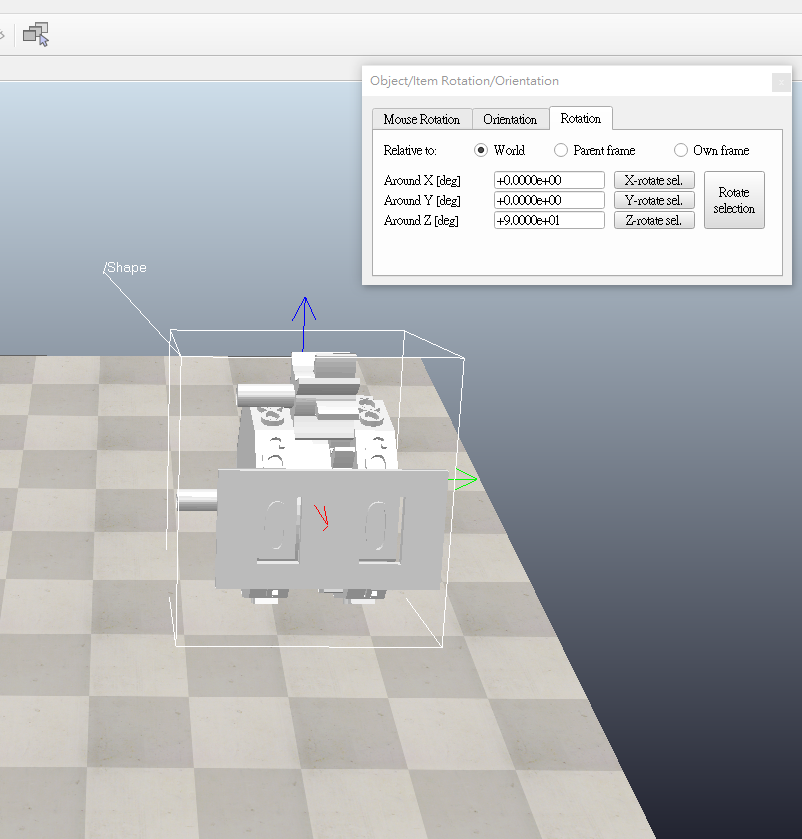
\includegraphics[width=15cm]{12}
\caption{\Large Example of injection mold made using a 3D printer (thefabricator.com) 使用 3D 列印機製作射出成型模具的範例 (thefabricator.com)}\label{fig.12}
\end{center}
\end{figure}
\newpage

\fontsize{14pt}{2.5pt}\sectionef 
{Additive manufacturing has become an incredible tool for ultra-flexible production. This mindset of continuous improvement, especially when regarding prototyping and iterative design, is a hallmark of the lean mentality that is so relevant in the modern industry.}\\[10pt]

\fontsize{14pt}{5pt}\sectionef
 {增材製造已成為超靈活生產的不可思議的工具。這種持續改進的心態,特別是在原型設計和迭代設計方面,是與現代工業密切相關的精益心態的標誌。
}\\[15pt]

\fontsize{14pt}{2.5pt}\sectionef 
{As mentioned in the previous section, in this case study it is considered the creation of a new product and its production process by the fictional company. This product consists in a plastic small form factor computer case, composed of 3 different parts (Figure 13) that are expected to be designed and prototyped considering combination of additive manufacturing and CNC milling towards a plastic injection molding production.}\\[10pt]

\fontsize{14pt}{5pt}\sectionef
 {如上一節所提到的,在本案例研究中,它被視為虛構公司的新產品的創造及其生產過程。該產品由一個塑膠小型電腦機殼組成,由 3 個不同的部件組成(圖 13),預計在設計和原型製作時考慮將增材製造和 CNC 銑削相結合進行塑膠射出成型生產。
}\\[25pt]

\begin{figure}[hbt!]
\begin{center}
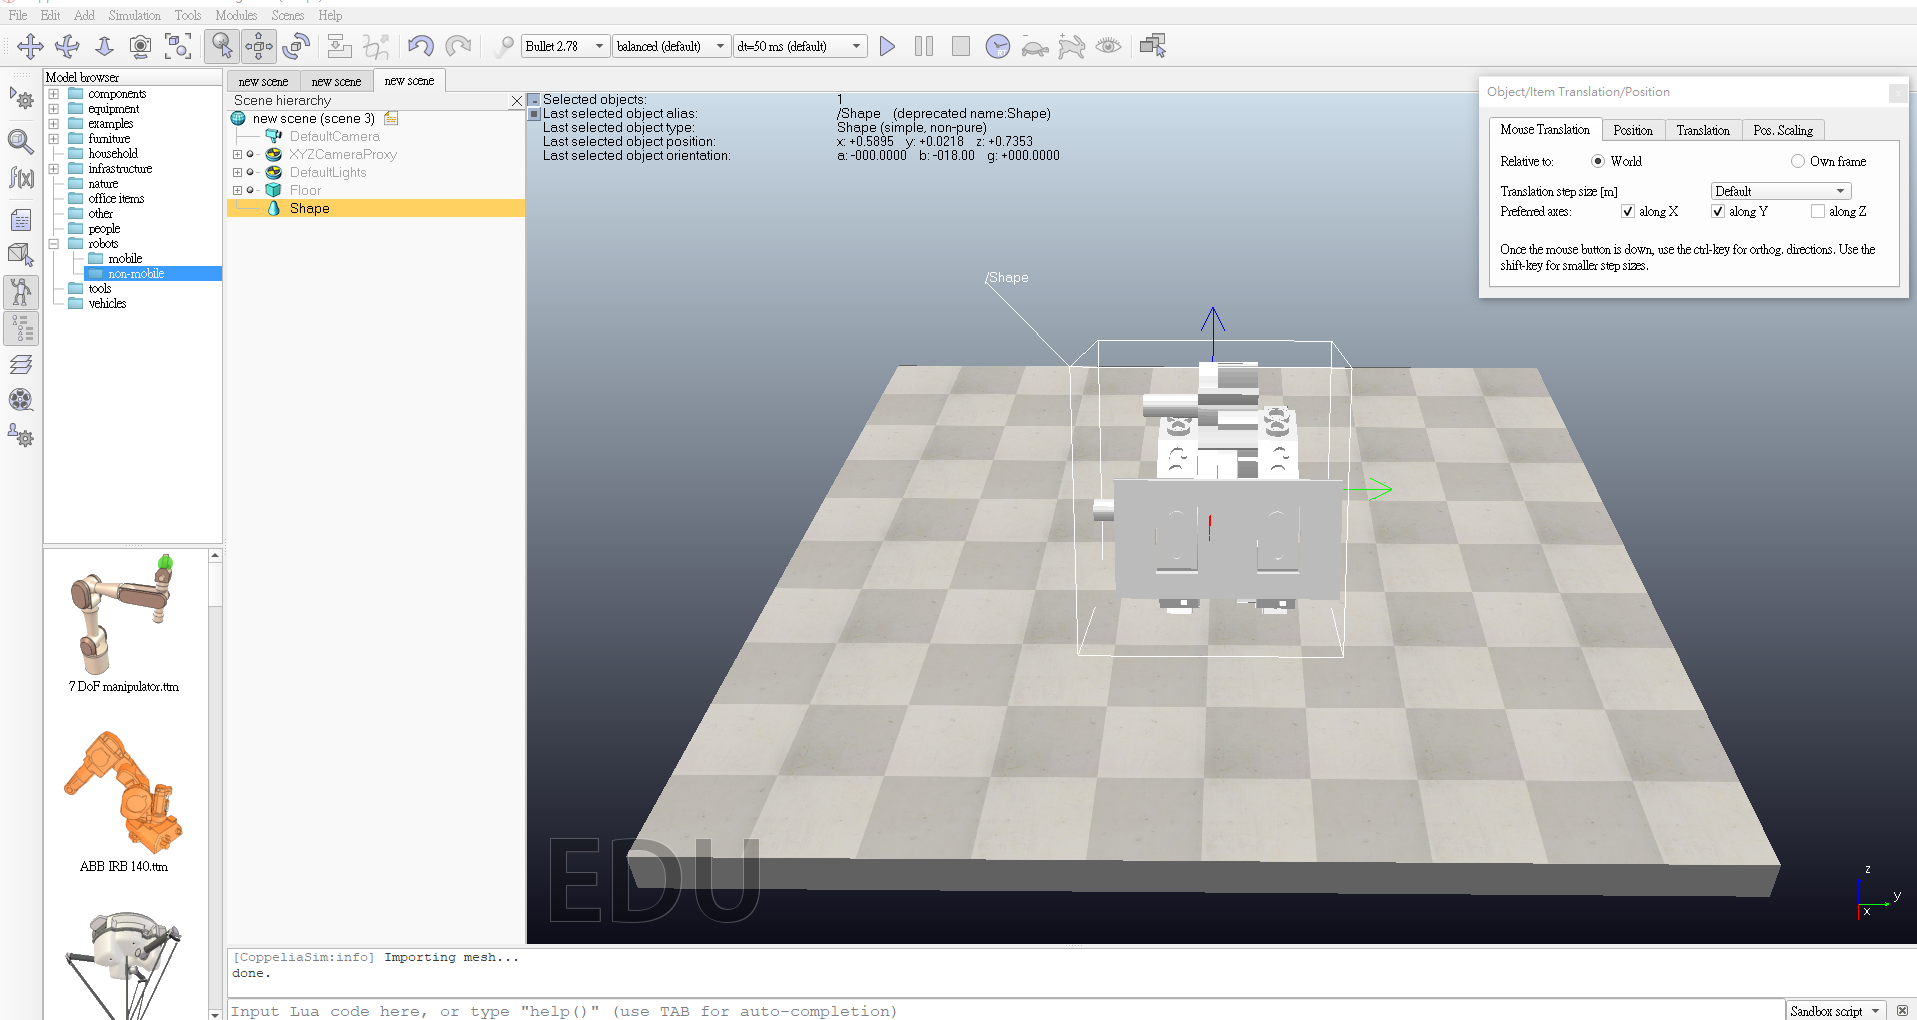
\includegraphics[width=15cm]{13}
\caption{\Large 3D exploded view of the theoretical product 理論產品的 3D 分解圖}\label{fig.13}
\end{center}
\end{figure}
\newpage

\subsection{Part A A部分}

\fontsize{14pt}{2.5pt}\sectionef 
{PART-A (Figure 14) is the core structure of the computer case. It is expected to comport all the pieces necessary for the proper function of the small form factor computer in question. To this end a raw material A was selected to be Acrylonitrile Butadiene Styrene (ABS) this is an opaque thermoplastic polymer and an engineering grade plastic. It is commonly used to produce electronic parts such as phone adaptors, keyboard keys and wall socket plastic guards.}\\[15pt]

\fontsize{14pt}{5pt}\sectionef
 {PART-A(圖14)是電腦機殼的核心結構。它預計將配備所討論的小型計算機正常運行所需的所有部件。為此,原料 A 被選為丙烯腈丁二烯苯乙烯 (ABS),這是一種不透明的熱塑性聚合物和工程級塑膠。它通常用於生產電子零件,例如電話適配器、鍵盤按鍵和牆壁插座塑膠防護罩。}\\[15pt]

\begin{figure}[hbt!]
\begin{center}
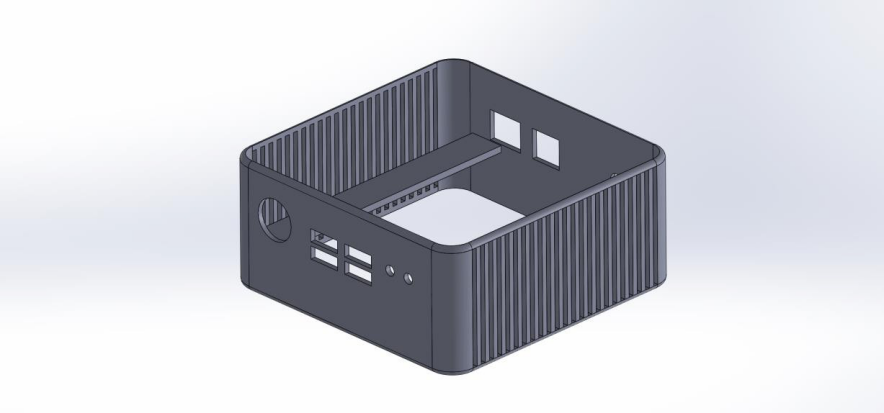
\includegraphics[width=15cm]{14}
\caption{\Large Isometric view of Part A A 部分等距視圖}\label{fig.14}
\end{center}
\end{figure}
\vspace{1cm}

\fontsize{14pt}{2.5pt}\sectionef 
{The main reasons for choosing this material specifically are its toughness, its good dimensional stability (resistance to change dimensions after cooling), its high impact resistance and surface hardness. Finally, it is also commonly available in the form of 3D printing filament for extrusion 3D printers which should prove to be quite useful during prototyping.}\\[15pt]

\fontsize{14pt}{5pt}\sectionef
 {特別選擇這種材料的主要原因是其韌性、良好的尺寸穩定性(冷卻後不易改變尺寸)、高抗衝擊性和表面硬度。最後,它通常也以用於擠出 3D 列印機的 3D 列印絲的形式提供,這在原型製作過程中應該非常有用。}\\[15pt]
\newpage

\subsection{Part B and C     B 部分和 C 部分}

\fontsize{14pt}{2.5pt}\sectionef 
{Parts B and C are lids that should snap into place, closing the system. These are very simple pieces and require a certain level of elasticity so it can deform to assure a screwless assembly. These two identical parts are going to be made with Thermoplastic Polyurethane (TPU), because of its elastic nature and great tensile and tear strength. This sort of polymer is often used to produce parts that demand a rubber-like elasticity. TPU performs well at high temperatures and is commonly used in power tools, cable insulations and sporting goods. Finally, TPU is also available in the form of filament for 3D printers which, for the simulation, will be used for prototyping.}\\[15pt]

\fontsize{14pt}{5pt}\sectionef
 {B 和 C 部分是蓋子,應卡入到位,關閉系統。這些都是非常簡單的零件,需要一定程度的彈性,以便可以變形以確保無螺絲組裝。這兩個相同的部件將由熱塑性聚氨酯 (TPU) 製成,因為它具有彈性、拉伸強度和撕裂強度。這種聚合物通常用於生產需要類似橡膠彈性的零件。 TPU 在高溫下表現良好,常用於電動工具、電纜絕緣材料和體育用品。最後,TPU 還可以以細絲的形式用於 3D 列印機,用於模擬,用於原型製作。}\\[15pt]

\begin{figure}[hbt!]
\begin{center}
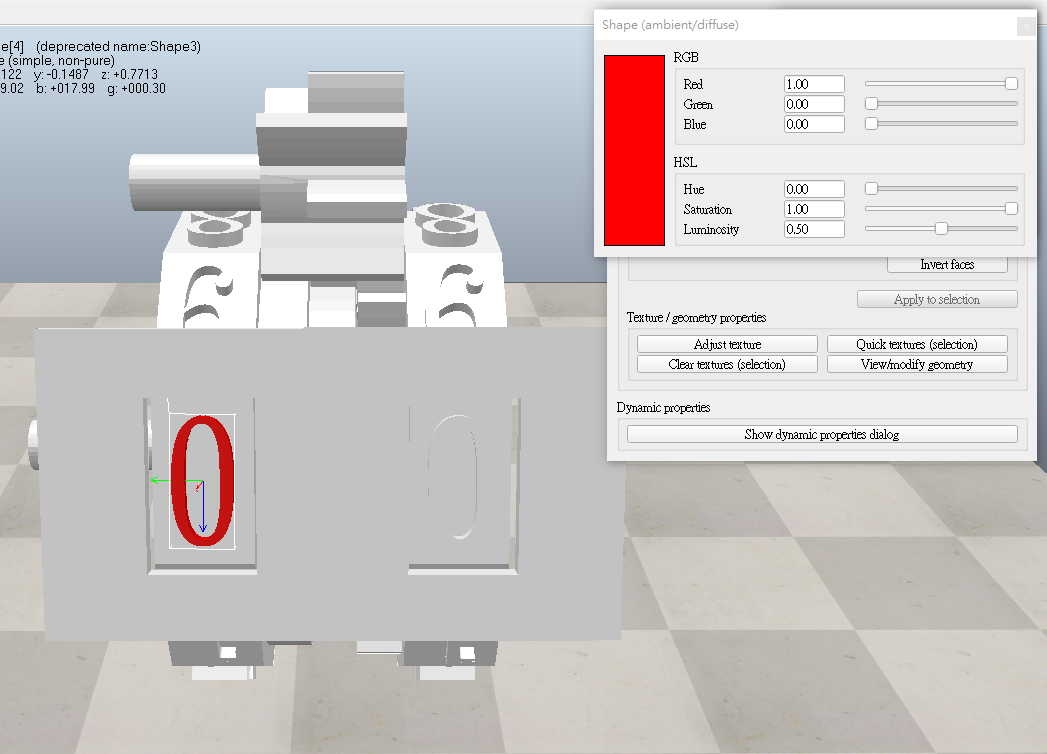
\includegraphics[width=15cm]{15}
\caption{\Large Part B and C     B 部分和 C 部分}\label{fig.15}
\end{center}
\end{figure}

\subsection{Molds 模具}

\fontsize{14pt}{2.5pt}\sectionef 
{Ideally all molds should be made of steel, for longevity of the mold and product quality. That being said, the injected plastics that are being selected for all parts are not so pressure dependent and their forms are not so complex, so it is assumed that aluminum molds made with a precision CNC machining should suffice to produce said parts.}\\[10pt]

\fontsize{14pt}{5pt}\sectionef
 {理想情況下,所有模具應由鋼製成,以確保模具的使用壽命和產品品質。話雖如此,為所有零件選擇的注射塑膠並不那麼依賴壓力,而且它們的形狀也不是那麼複雜,因此假設用精密 CNC 加工製造的鋁模具應該足以生產所述零件。}\\[15pt]

\fontsize{14pt}{2.5pt}\sectionef 
{It is also assumed that all molds are simple enough to be prototyped using 3D printing. Although this is not always true, it was determined representative enough for this simulation. The type of material used in those prototypes is high temperature resign cured using an SLA 3DPrinter. Additionally, the mold will be considered the main physical aspect to be developed when regarding the production process because it something that directly affects the production as well as something that can be produced in house and tracked as a product would.}\\[10pt]

\fontsize{14pt}{5pt}\sectionef
 {也假設所有模具都足夠簡單,可以使用 3D 列印來製作原型。儘管這並不總是正確的,但它對於本次模擬來說具有足夠的代表性。這些原型中使用的材料類型是使用 SLA 3D 列印機進行高溫重新固化的。此外,在生產過程中,模具將被視為要開發的主要物理方面,因為它直接影響生產,並且可以像產品一樣在內部生產和追蹤。}\\[15pt]

\section{What is analized during the simulation 模擬過程中分析了什麼}

\fontsize{14pt}{2.5pt}\sectionef 
{Taking into consideration the diagram, shown in Figure 9, as well as the main aspects of a successful integration of PLM and MES as described in the section 3.1, this experiment aims to produce commentary regarding the following relevant questions in Table 1.}\\[10pt]

\fontsize{14pt}{5pt}\sectionef
 {考慮到圖 9 所示的圖表,以及第 3.1 節中描述的 PLM 和 MES 成功整合的主要方面,本實驗旨在對錶 1 中的以下相關問題進行評論。}\\[15pt]

\begin{center}
 \fontsize{16}{16}\selectfont \textbf{Table 1 Summary of questions to be answered}\\
\fontsize{16}{16}\selectfont \textbf{表1 需回答的問題總表}\\
\end{center}

\begin{figure}[hbt!]
\begin{center}
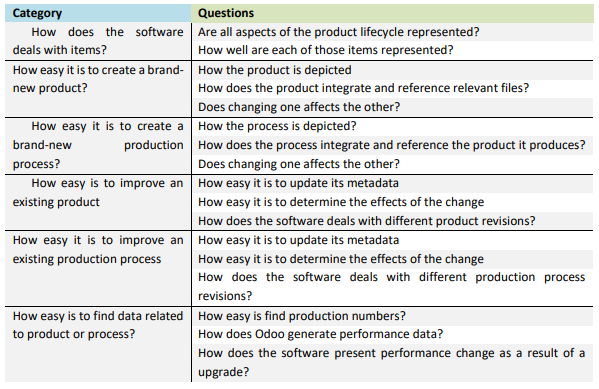
\includegraphics[width=15cm]{15-2}
\end{center}
\end{figure}

\newpage



\begin{table}[htbp]
    \centering
    \label{tab:example}
    \begin{tabular}{|c|c|}
        \hline
        類別 & 問題 \\
        \hline
        軟體如何處理物品? & 是否代表了產品生命週期的所有面向? \\
         & 這些項目的表現如何?\\
         \hline
        創造一個全新的產品有多容易? & 產品的描述方式? \\
         & 產品如何整合和引用相關文件?\\
         & 改變一個會影響另一個嗎? \\
         \hline
       創造一個是多麼容易全新的生產流程? & 其過程是如何描述的? \\
         & 該流程如何整合和參考其生產的產品?\\
         & 改變一個會影響另一個嗎? \\
         \hline
        改進現有產品有多容易? & 更新元數據有多容易? \\
         & 確定變更的影響有多容易? \\
         & 軟體如何處理不同的產品版本? \\
        \hline
        改進現有生產流程有多容易? & 更新元數據有多容易? \\
         & 確定變更的影響有多容易?\\
         & 軟體如何因應不同的生產流程修訂?\? \\
        \hline
        尋找與產品或流程相關的數據有多容易? & 要找出生產編號有多容易? \\
         & Odoo 如何產生效能數據? \\
         & 軟體如何呈現效能變化升級? \\
        \hline
    \end{tabular}
\end{table}




\newpage
\chapter{THE ODOO SOFTWARE} 
\pagenumbering{arabic} %設定頁號阿拉伯數字
\setcounter{page}{26}  %設定頁數
\begin{center}
\fontsize{18}{16}\selectfont \textbf{ODOO 軟體}\\
\end{center}


\section{Introduction to the Odoo software ODOO軟體簡介}
\fontsize{12}{2.5pt}\sectionef  
{Odoo is a commercial business management software with strong ties to the open source community. Initially started as open source ERP software becoming well received as an affordable and intuitive package that thrived on integration and expandability. Since then, as the company experienced accelerated growth, it shifted their business model to include an enterprise paid version as well as an online service.}\\[1pt]

\fontsize{12}{2.5pt}\sectionef 
{本論文的目的是透過分析包含所述整合的不同概念和動態,找出使用現成的 Odoo 軟體可以實現 PLM+MES 系統的程度,並應用一個虛構的場景來確定這些概念是否以及哪些概念包含在此打包解決方案中。}\\[15pt]

\fontsize{12}{2.5pt}\sectionef
{To contextualize, the Odoo software differs from other solutions in the market substantially both in implementation and business model. To summarize, the Odoo software 
was originated as an open-source ERP software as oppose to a PLM or MES software and as such its availability and modularity are reasonably expanded. It goes without saying that the counter point for this that its usability in the field of PLM or MES is uncertain hence the value of this work.}\\[1pt]

\fontsize{12}{2.5pt}\sectionef  
{如同 2.2 節中所提到的,現代 ERP 系統通常是模組化的,並且在以 Odoo 為例,由於數量驚人,這種模組化尤為明顯
由社區開發的模組以及公司開發的模組提供的擴展模組高度整合。 這種可擴展性使得該軟體如此重要回到 PLM+MES 整合的主題,因為現有的 PLM 模組以及其製造模組中具有顯著的 MES 功能。}\\[15pt]

\fontsize{12}{2.5pt}\sectionef  
{Within the scope of this thesis, the objective is to utilize this software on the management of the previously mentioned fictional company and draw conclusions regarding how effective the integration of PLM and MES is already present within this system.  }\\[1pt]

\fontsize{12}{2.5pt}\sectionef 
{在本論文的範圍內,目標是利用該軟體進行管理前面提到的虛構公司,並就其有效性得出結論PLM 和 MES 的整合已經存在於該系統中。}\\[15pt]

\section{How it works 如何運作 }
\fontsize{12}{2.5pt}\sectionef 
 {The software can be installed in most x86 computers and it supports several operating
systems including windows and all the main Linux distributions.}\\[1pt]

\fontsize{12}{2.5pt}\sectionef  
{該軟體可以安裝在大多數x86電腦上,並且支援多種操作
系統包括 Windows 和所有主要的 Linux 發行版。}\\[15pt]

\fontsize{12}{2.5pt}\sectionef 
 {Ideally, the Odoo software is installed in a computer connected to a local area networkand starts a SQLdatabase that holds all the necessary information and files produced by thebusiness (Figure 16). Said computer works essentially as a server and accessed via abrowser by the other machines present in the network. This computer can be a dedicatedserver or a working desktop in use, but it is important to remember that it must remain ONand connected throughout the entire time the software is required to function.}\\[1pt]

\fontsize{12}{2.5pt}\sectionef  
{理想情況下,Odoo 軟體安裝在連接到區域網路的電腦上並啟動一個 SQL 資料庫,其中包含由該程式產生的所有必要資訊和文件業務(圖 16)。 所述計算機本質上作為伺服器工作並透過網路中其他機器的瀏覽器。 這台計算機可以是專用的伺服器或正在使用的工作桌面,但重要的是要記住它必須保持開啟狀態並且在軟體需要運作的整個過程中都保持連線。}
\\[15pt]


\begin{figure}[hbt!]
\begin{center}
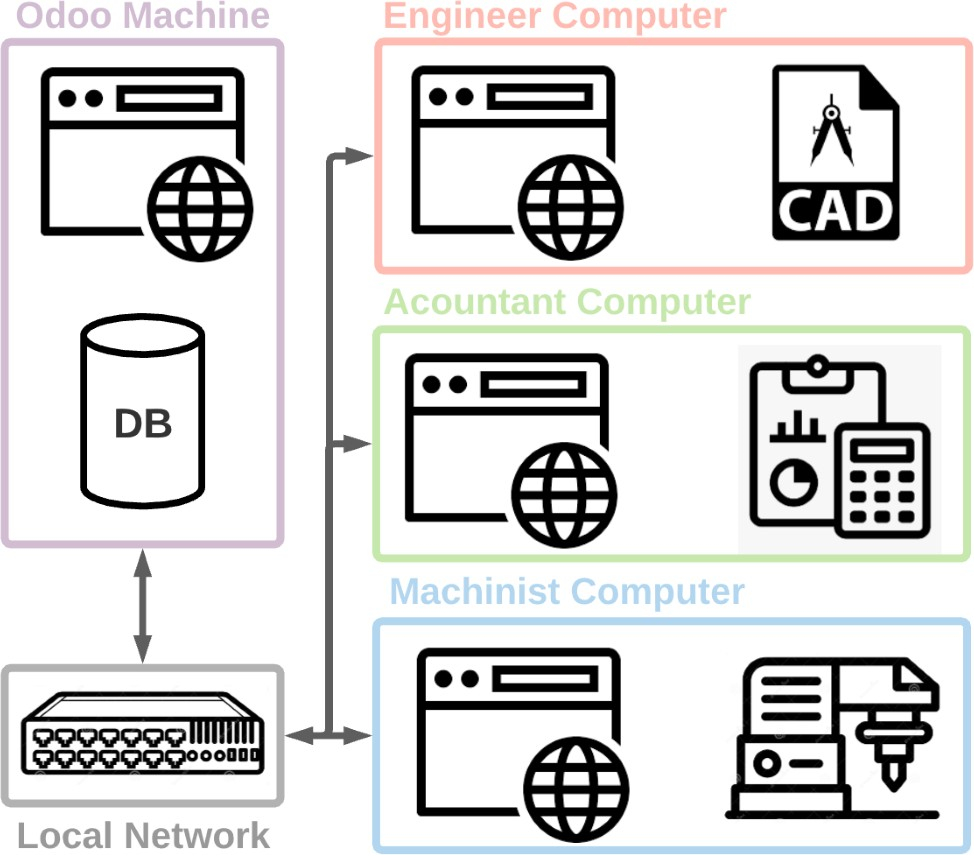
\includegraphics[width=15cm]{16}
\caption{\Large  Function Diagram of Odoo configuration A Odoo配置A功能圖}\label{fig.16}
\end{center}
\end{figure}


\fontsize{12}{2.5pt}\sectionef 
 {Another option is to use the hosting service provided by Odoo SA (Figure 17). In this case
the system would be hosted by them and data would be stored in their cloud. This is a good
fit for many small businesses specially if they are particularly fond of the website related
modules (used to build and manage web sites and e-stores). It is however network dependent
which may pose a problem in some instances.}\\[1pt]

\fontsize{12}{2.5pt}\sectionef  
{另一個選擇是使用 Odoo SA 提供的託管服務(圖 17)。 在這種情況下
該系統將由他們託管,數據將儲存在他們的雲端中。 這是一個很好的
適合許多小型企業,特別是如果他們特別喜歡相關網站
模組(用於建立和管理網站和電子商店)。 然而,它依賴於網絡
這在某些情況下可能會造成問題。}
\\[15pt]


\begin{figure}[hbt!]
\begin{center}
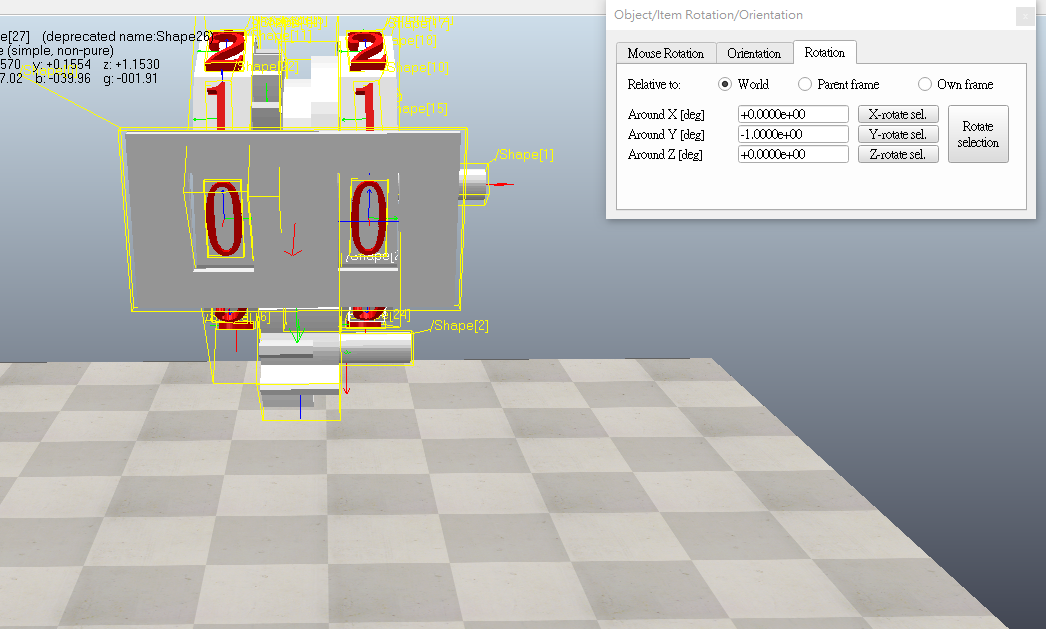
\includegraphics[width=15cm]{17}
\caption{\Large  Function Diagram of Odoo configuration B Odoo配置B功能圖}\label{fig.17}
\end{center}
\end{figure}

\fontsize{12}{2.5pt}\sectionef 
 {Users essentially interact with the system through the graphical user interface (GUI) and
use it to access the different modules available as need by a per user basis. This means that
restrictions can be applied to different users in order to maintain control over the different
aspects of the business activity, e.g., accountants would get access to accounting module,
sales module and inventory module but they would be restricted from the manufacturing
module. This sort of restriction guarantees control over the processes only to the proper
employees.}\\[1pt]

\fontsize{12}{2.5pt}\sectionef  
{使用者本質上是透過圖形使用者介面(GUI)與系統互動的使用它可以根據每個用戶的需要存取可用的不同模組。 這意味著可以對不同的使用者套用限制,以維持對不同使用者的控制業務活動的各個方面,例如會計師可以存取會計模組,銷售模組和庫存模組,但它們將被限制在製造中模組。 這種限制保證了只有適當的人才能控制流程僱員。}
\\[15pt]


\fontsize{12}{2.5pt}\sectionef 
 {Within said GUI the different modules appear as app icons (Figure 18) and, from the getgo, the company has available a reasonable selection of well-integrated applications not to mention a vast app store filled with community made modules.}\\[1pt]

\fontsize{12}{2.5pt}\sectionef  
{在所述GUI 中,不同的模組顯示為應用程式圖標(圖18),並且從一開始,該公司就提供了合理的整合良好的應用程式選擇,更不用說充滿社區製作模組的龐大應用程式商店。}
\\[15pt]


\begin{figure}[hbt!]
\begin{center}
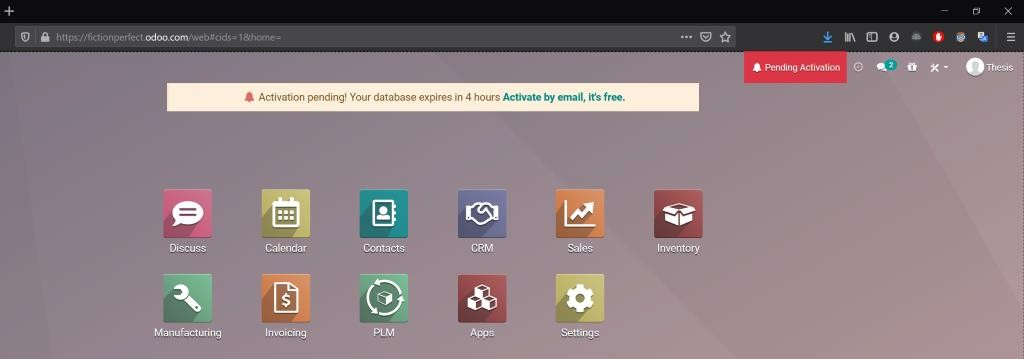
\includegraphics[width=15cm]{18}
\caption{\Large Screenshot of GUI from Odoo in configuration B 配置 B 中 Odoo 的 GUI 螢幕截圖}\label{fig.18}
\end{center}
\end{figure}

\section{Odoo’s view on manufacturing: Odoo 對製造業的看法:}


\fontsize{12}{2.5pt}\sectionef 
 {Odoo considers that the responsibilities regarding manufacturing of anything is distributed throughout different company departments, each of which is responsible for
specific file types and dealt with using specific apps (Table 2). From the perspective of PLM this is very positive because as mentioned by (Saaksvuori and Immonen, 2008) about User privilege management – the PLM system is used to define information access and maintenance rights. The PLM system defines the people who can create new information or make, check and accept changes, and those who are allowed only to view the information or documents in the system. user privilege management is usually a challenge when regardingintegration of PLM with other systems.}\\[1pt]

\fontsize{12}{2.5pt}\sectionef  
{Odoo 認為任何產品製造的責任都是分佈在公司不同部門,各部門負責特定的文件類型並使用特定的應用程式進行處理(表 2)。 從PLM的角度來看這是非常正面的,因為正如(Saaksvuori 和 Immonen,2008)關於使用者所提到的權限管理-PLM系統用於定義資訊存取和維護權利。 PLM 系統定義了可以建立新資訊或進行、檢查和接受更改,以及那些僅被允許查看資訊或系統中的文件。 使用者權限管理通常是一個挑戰PLM 與其他系統的整合。}
\\[15pt]


\begin{table}[htbp]
    \centering
    \begin{tabular}{|c|c|}
        \hline
         Department 部門& Documents/Apps 文件/應用程式\\
        \hline
        Engineering  工程& CAD BOM CAD 和物料清單 \\
        Manufacturing Engineering  製造工程& Routings, Worksheets, Workcenters 工藝路線、工作表、工作中心\\
       Purchase/Procurement 採購/採購& Procurement order, Request for quotation 採購訂單、詢價單\\
       Inventory Operators 庫存操作員&Receipt, Barcode 收據、條碼 \\
       Manufacturing Foreman 製造工長& Manufacturing order, Planning 製造訂單、計劃 \\
       Manufacturing Operators 製造經營者& Work order工作指示 \\
       Inventory Operators 庫存操作員& Delivery送貨 \\
       Quality 品質& Alert, Analysis, Control points 警報、分析、控制點\\、
      Engineering  工程& Engineering change order工程變更單 \\
      Maintenance 維護& Preventive/Corrective 預防/糾正\\
        \hline
    \end{tabular}
\end{table}


\fontsize{12}{2.5pt}\sectionef 
 {From Odoo’s perspective in the beginning of any usual manufacturing process, the first
step will be the engineers designing the product usually using a CAD software. Once that is
done, they will create a Bill of materials (BOM) this is a list of components or materials
necessary to produce the product. At this point the focus goes to the manufacturing process
itself.}\\[1pt]

\fontsize{12}{2.5pt}\sectionef  
{從 Odoo 的角度來看,在任何通常的製造過程開始時,第一個
步驟是工程師通常使用 CAD 軟體設計產品。 一旦那是
完成後,他們將創建物料清單 (BOM),這是組件或材料的列表
生產產品所必需的。 此時重點轉向製造過程
本身。}
\\[15pt]

\fontsize{12}{2.5pt}\sectionef 
 {The software view of process is focused on routings, worksheets and work centers this is
done by the manufacturing engineering team. A routing is a set of steps a product goes
through for production. Worksheets are the instructions for the manufacturing operator, and
work centers are the places where the production is being conducted. Odoo considers that
these are the requirements for putting engineers plans in motion}\\[1pt]

\fontsize{12}{2.5pt}\sectionef  
{流程的軟體視圖側重於工藝路線、工作表和工作中心,這是
由製造工程團隊完成。 製程路線是產品運作的一組步驟
透過進行生產。 工作表是給製造操作員的說明,並且
工作中心是進行生產的地方。 奧杜認為
這些是實施工程師計劃的要求}
\\[15pt]

\fontsize{12}{2.5pt}\sectionef 
 {A procurement department will be responsible for requesting for quotations (RFQ) or
purchase orders (PO). Inventory operators take care of receipts based on those POs, which is
usually done using a barcode application within Odoo. As explained in the first section of
this chapter Odoo is primarily an ERP system and it is at this point that it is possible to notice
some ERP centric characteristics like the focus on inventory and management of resources.
This will be further analyzed in the following sections, but it is fair to point out that those
RFQ and PO are considered items within the data base.}\\[1pt]

\fontsize{12}{2.5pt}\sectionef  
{採購部門將負責索取報價(RFQ)或
採購訂單 (PO)。 庫存操作員根據這些 PO 處理收貨,即
通常使用 Odoo 中的條碼應用程式完成。 正如第一節所解釋的
本章 Odoo 主要是一個 ERP 系統,此時可以注意到
一些以 ERP 為中心的特徵,例如專注於庫存和資源管理。
這將在以下各節中進一步分析,但公平地指出,這些
RFQ 和 PO 被視為資料庫中的項目。}
\\[15pt]

\fontsize{12}{2.5pt}\sectionef 
 {Only when you have the design the process and the materials required Odoo considers
manufacturing possible. Then the manufacturing foreman will create a manufacturing order
(MO) and manage the planning of the manufacturing operators through work orders (WO)
and work centers. Then the manufacturing operators can start production following a work
order. After the products are produced, they automatically appear in the inventory database
which alongside packaging and delivery is managed by the Inventory department.}\\[1pt]

\fontsize{12}{2.5pt}\sectionef  
{只有當您設計了 Odoo 考慮的流程和所需材料時
製造成為可能。 然後製造工長將創建製造訂單
(MO) 並透過工單管理製造操作員的計畫 (WO)
和工作中心。 然後製造操作員可以在工作結束後開始生產
命令。 產品生產出來後,自動出現在庫存資料庫中
與包裝和交付一起由庫存部門管理。}
\\[15pt]


\fontsize{12}{2.5pt}\sectionef 
 {Odoo considers that quality team is responsible for assign control/check points as well as
identify possible issues within the product or production. These quality control check points
are very interesting from the MES perspective because it represents valuable production data
that is collected in real time as production occurs, i.e., it is possible to assign a dimension
check after the production of every piece where the machinist will fill in the dimensions to
track quality over time.}\\[1pt]

\fontsize{12}{2.5pt}\sectionef  
{Odoo 認為品質團隊負責分配控制/檢查點以及
識別產品或生產中可能存在的問題。 這些品質控制檢查點
從 MES 的角度來看非常有趣,因為它代表了有價值的生產數據
在生產發生時即時收集,即可以分配維度
每件產品生產完成後進行檢查,機械師將填寫尺寸
隨著時間的推移跟踪品質。}
\\[15pt]


\fontsize{12}{2.5pt}\sectionef 
 {If it's a problem of design or if there is possibility for improvement an engineering change
order (ECO) can be issued. This falls back to the hands of the manufacturing engineering
team and will focus on updating documents and the BOM. The ECO is the heart of how Odoo
deals with tracking change within the system. That is key when regarding PLM and in fact is
the focus of the Odoo application called PLM. To which lengths said application is capable
to perform is the subject of the next section.}\\[1pt]

\fontsize{12}{2.5pt}\sectionef  
{如果是設計問題或是否有改進工程變更的可能性
可以發出訂單(ECO)。 這又回到了製造工程的手中
團隊將專注於更新文件和 BOM。 ECO 是 Odoo 的核心
處理追蹤系統內的變化。 對於 PLM 而言,這是關鍵,事實上
Odoo 應用程式的焦點稱為 PLM。 所述應用程式能夠達到什麼長度
執行是下一節的主題。}
\\[15pt]

\section{The information structure of Odoo Odoo的資訊結構 }

\fontsize{12}{2.5pt}\sectionef 
 {Each module focuses in the manipulation of specific object-oriented classes that hold
metadata within the database. These are the virtual Items that are responsible for virtualizing
the aspects of the product lifecycle as referred by in (Section 3.1). Different types of items
have different types of accounts and hold different sorts of data, i.e., a product item is
representative of a certain product and holds metadata that is relevant to its interactions and
use as well as links to other possible items that are closely relevant like their responsible user
or the bill of materials necessary to its manufacturing. Odoo them makes all that information
accessible and interactable through its browser interface (Figure 19 and Figure 20). For the
sake of consistency this document will refer to specific item representations (E.g. Bolt) as
‘item’ and refer to a type of item (Product) as ‘item class’.}\\[1pt]

\fontsize{12}{2.5pt}\sectionef  
{每個模組都專注於特定物件導向類別的操作,這些類別包含
資料庫內的元資料。 這些都是負責虛擬化的虛擬項
(第 3.1 節)中提到的產品生命週期的各個面向。 不同類型的物品
擁有不同類型的帳戶並保存不同類型的數據,即產品項目是
代表某個產品並保存與其互動相關的元數據
使用以及指向其他可能的項目的鏈接,這些項目與其負責的用戶密切相關
或其製造所需的物料清單。 Odoo 他們製作了所有這些資訊
可透過其瀏覽器介面進行存取和互動(圖 19 和圖 20)。 為了
為了保持一致性,本文檔將特定的項目表示(例如螺栓)稱為
「item」並將某種類型的項目(產品)稱為「項目類別」。}\\[15pt]

\begin{figure}[hbt!]
\begin{center}
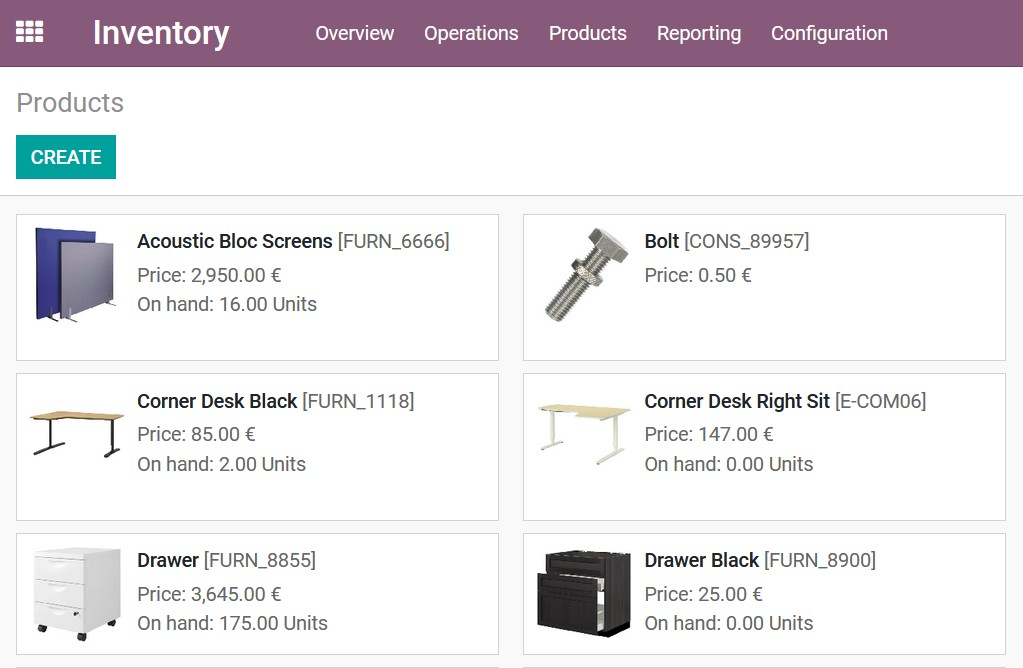
\includegraphics[width=15cm]{19}
\caption{\Large Example of Odoo’s interface regarding items Odoo 有關專案的介面範例}\label{fig.19}
\end{center}
\end{figure}

\begin{figure}[hbt!]
\begin{center}
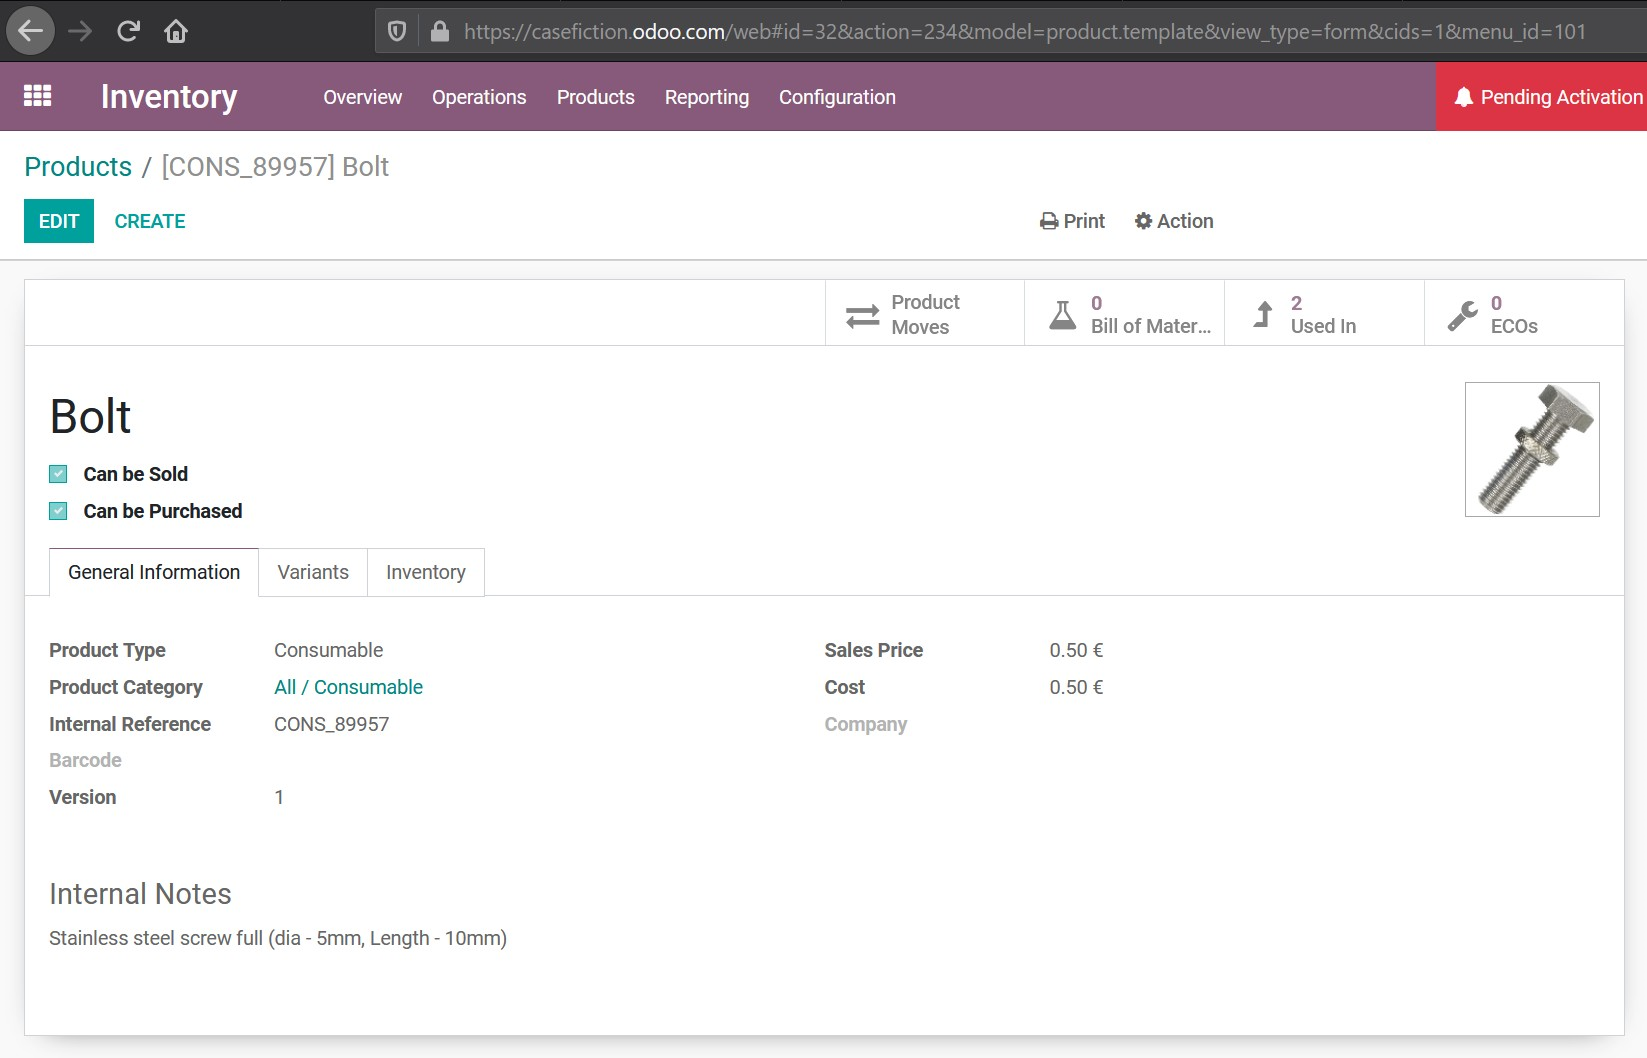
\includegraphics[width=15cm]{20}
\caption{\Large Example of specific item and its metadata as displayed by GUI GUI 顯示的特定項目及其元資料的範例}\label{fig.20}
\end{center}
\end{figure}


\fontsize{12}{2.5pt}\sectionef 
 {Within Odoo, there are several types of those item classes (some holding a lot of metadata
and some holding very little) all with a varying degree of relationships and integration. Since
the scope of this work is limited to the PLM and MES capabilities, the focus is on the items
that are related to it. The following sections will provide short explanations for the main 7
item classes of Odoo’s manufacturing process since its basic understanding is helpful for the
reader to follow the simulation. These are represented in the following diagram (Figure 21).
Other items that are external to the manufacturing procedure will be presented throughout
the simulation.}\\[1pt]

\fontsize{12}{2.5pt}\sectionef  
{在 Odoo 中,這些項目類有多種類型(有些包含大量元資料)
有些持有很少),所有這些都具有不同程度的關係和整合。 自從
這項工作的範圍僅限於 PLM 和 MES 功能,重點是專案
與它相關的。 以下部分將對主要 7 個部分進行簡短說明
Odoo 製造流程的專案類別,因為它的基本了解有助於
讀者跟隨模擬。 這些如下圖所示(圖 21)。
製造過程之外的其他項目將在整個過程中呈現
模擬。}\\[15pt]


\begin{figure}[hbt!]
\begin{center}
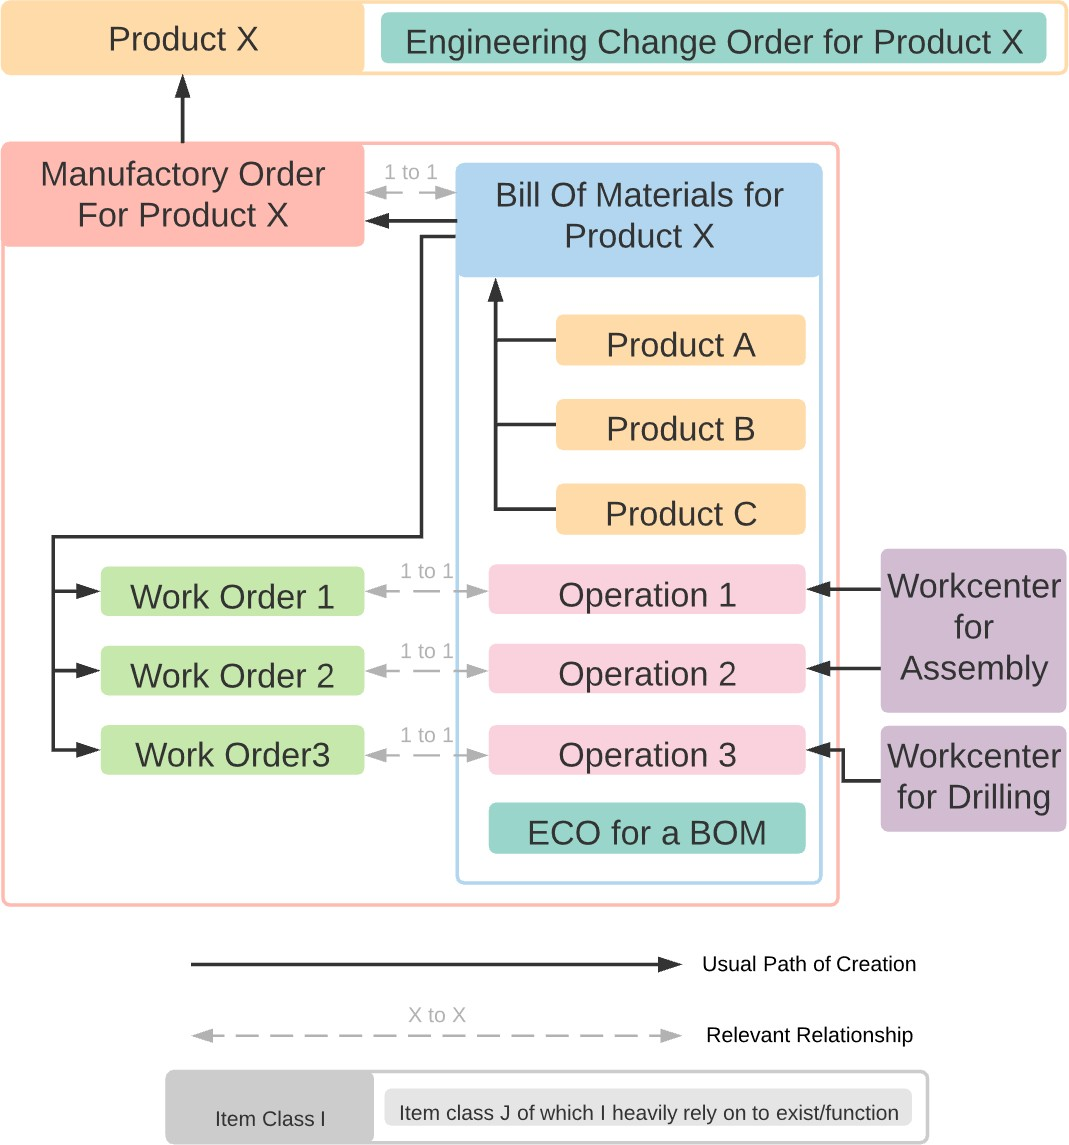
\includegraphics[width=15cm]{21}
\caption{\Large Simplified Item relation diagram to the manufacturing of a product X  與產品 X 的製造相關的簡化專案關係圖}\label{fig.21}
\end{center}
\end{figure}



\section{Product Item 產品項目 }

\fontsize{12}{2.5pt}\sectionef 
 {Every material, component or product is characterized by a PRODUCT type class that is
held and mainly managed within the Inventory application of Odoo. That means that within
the system product production is dependent on the availability of other products that are
either bought as they are or manufactured from another products (Figure 22), i.e., raw
materials are considered products as well, more specifically products that are purchased and
then included in the BOM’s to manufacture other products. This is considered the main item
class since it is both the source and the goal of manufacturing.
}\\[1pt]

\fontsize{12}{2.5pt}\sectionef  
{每種材料、組件或產品都具有一個產品類型類別,該類別是
主要在 Odoo 的庫存應用程式中進行持有和管理。 這意味著在
系統產品的生產取決於其他產品的可用性
要麼按原樣購買,要麼用其他產品製造(圖 22),即原料
材料也被視為產品,更具體地說,是購買和使用的產品
然後包含在 BOM 中以製造其他產品。 這被認為是主要項目
階級,因為它既是製造的源泉,也是製造的目標。}\\[15pt]


\begin{figure}[hbt!]
\begin{center}
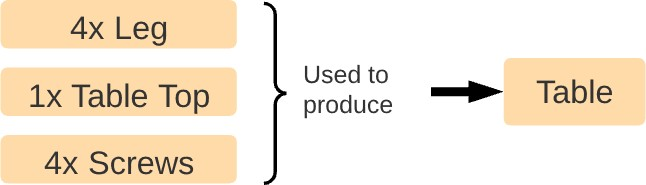
\includegraphics[width=15cm]{22}
\caption{\Large  simplified Product relation diagram  簡化的產品關係圖}\label{fig.22}
\end{center}
\end{figure}


\section{Operation item class and workcenter item class 操作項目類和工作中心項目類}

\fontsize{12}{2.5pt}\sectionef 
 {The operation item is representative of a manufacturing operation that is required to
transform components or raw materials into a product or new component while the
workcenter item represents the place at which the operation takes place, e.g., a sanding wood
will be carried out in a sanding station (Figure 23) that has the proper equipment. The
workcenter is eventually used in Odoo as a time/equipment management tool in its
production planning. Basically, when the production center is at full capacity it puts
following processes on hold or redirects the processes to an alternative workcenter. The
operation item is also responsible for holding the instruction files that are consulted during
production. }\\[1pt]

\fontsize{12}{2.5pt}\sectionef  
{操作項目代表製造操作,需要
將組件或原料轉化為產品或新組件,同時
工作中心項代表進行操作的地點,例如打磨木材
將在具有適當設備的打磨站(圖 23)中進行。 這
workcenter 最終在 Odoo 中用作時間/設備管理工具
計劃生產。 基本上,當生產中心滿載運轉時,
追蹤暫停的流程或將流程重定向到備用工作中心。 這
操作項也負責保存操作過程中查閱的指令文件
生產。}\\[15pt]

\begin{figure}[hbt!]
\begin{center}
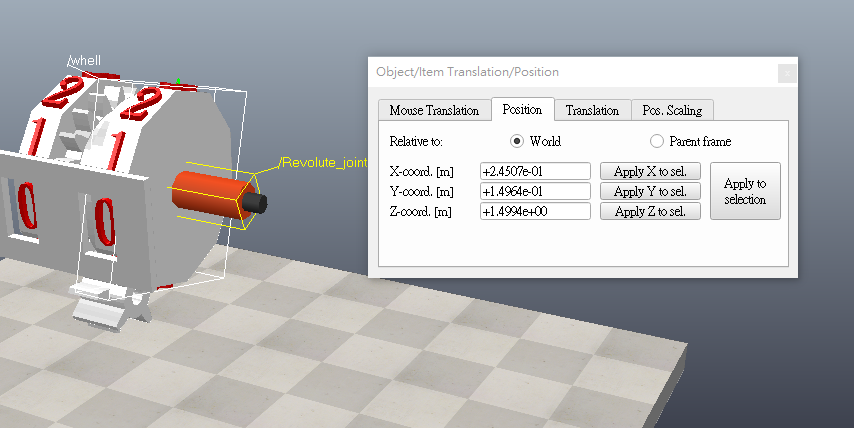
\includegraphics[width=15cm]{23}
\caption{\Large Simplified Operation diagram  簡化操作圖}\label{fig.23}
\end{center}
\end{figure}


\section{The Bill of Materials item class 物料清單項目類別 }

\fontsize{12}{2.5pt}\sectionef 
 {The Bill of Materials is a list of components necessary to build a product. In Odoo,
however, the BOM is best described by what PLM would consider the virtual representation
of the production process. That might seem counter intuitive at first considering the
previously mentioned operation item class, but in fact since the BOM is a compound item it
points directly to all item types necessary to produce the end product (Figure 24). For
example, let’s say that to build a product it is required 3 different parts and 4 different
operations; the BOM of said product would list all of them as well as specify the order in
which these are utilized.}\\[1pt]

\fontsize{12}{2.5pt}\sectionef  
{物料清單是建立產品所需組件的清單。 在奧杜,
然而,BOM 最好透過 PLM 認為的虛擬表示來描述
的生產過程。 乍一看,這似乎違反直覺
前面提到了操作項類,但實際上由於BOM是複合項它
直接指向生產最終產品所需的所有項目類型(圖 24)。 為了
例如,假設要建造一個產品,需要 3 個不同的部件和 4 個不同的部件
營運; 所述產品的 BOM 將列出所有這些產品並指定順序
這些都被利用了。}\\[15pt]

\begin{figure}[hbt!]
\begin{center}
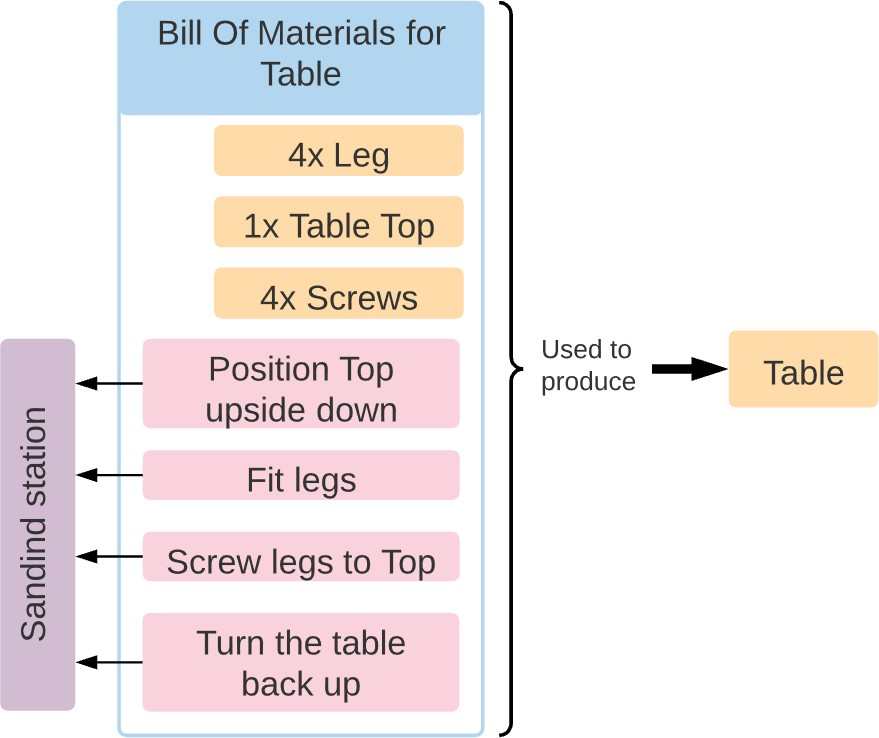
\includegraphics[width=15cm]{24}
\caption{\Large Simplified BOM diagram  簡化的 BOM 圖}\label{fig.24}
\end{center}
\end{figure}

\section{Manufacturing order item class and work order item class  製造訂單項目類和工作訂單項目類 }

\fontsize{12}{2.5pt}\sectionef 
 {Along the standard items that are considered within Odoo, orders are the ones that
represent commencement within the system. They are signaling that a change is taking place
somehow and somewhere. In the case of a manufacturing order it represents the order to
manufacture N number of specific products using it’s BOM as a base. It is as consequence
of that MO that work orders are automatically generated by Odoo (one for each necessary
operation listed in the BOM) and allocated throughout available necessary workcenters
(Figure 25). }\\[1pt]

\fontsize{12}{2.5pt}\sectionef  
{沿著 Odoo 中考慮的標準項目,訂單是那些
代表系統內的開始。 他們發出信號表明變化正在發生
以某種方式和某處。 在製造訂單的情況下,它代表訂單
使用 BOM 作為基礎製造 N 種特定產品。 其結果就是
該 MO 的工作訂單由 Odoo 自動產生(每個必要的工作訂單一個)
BOM 中列出的操作)並指派到可用的必要工作中心
(圖 25)。}\\[15pt]

\fontsize{12}{2.5pt}\sectionef 
 {The work order is the main form in which the manufacturing operators interact with Odoo,
it presents all the instructions specified by the operation item, as well as control towards its
completion. When a WO takes place the operator signals through the interface its beginning,
its completion and even any quality control check points required while the system keeps
track of timing and performance (Figure 26). Once all WO are done the MO can be declared
done and the materials and components specified in the BOM are consumed and the N copies
of the product is added to inventory. All that makes the work order a central piece as far as
MES is concerned.  }\\[1pt]

\fontsize{12}{2.5pt}\sectionef  
{工單是製造操作員與 Odoo 互動的主要形式,
它呈現了操作項指定的所有指令,以及對其的控制
完成。 當 WO 發生時,操作員透過介面發出開始訊號,
它的完成,甚至是系統保持時所需的任何品質控制檢查點
追蹤時間和性能(圖 26)。 一旦所有 WO 完成,即可宣布 MO
完成並且BOM中指定的材料和組件被消耗並且N份
產品的數量被加到庫存中。 所有這些使得工單成為核心部分
MES很在意。}\\[15pt]

\begin{figure}[hbt!]
\begin{center}
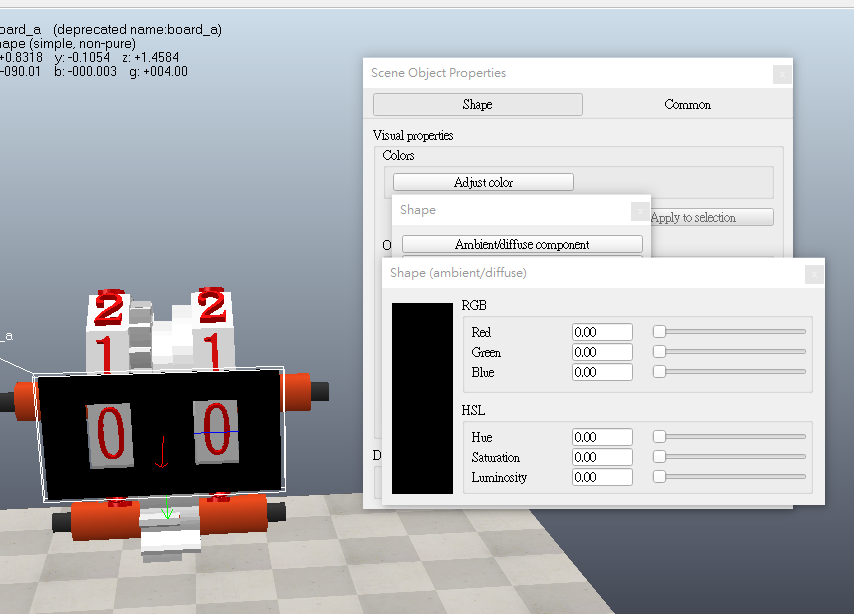
\includegraphics[width=15cm]{25}
\caption{\Large Simplified orders diagram  簡化訂單圖}\label{fig.25}
\end{center}
\end{figure}

\begin{figure}[hbt!]
\begin{center}
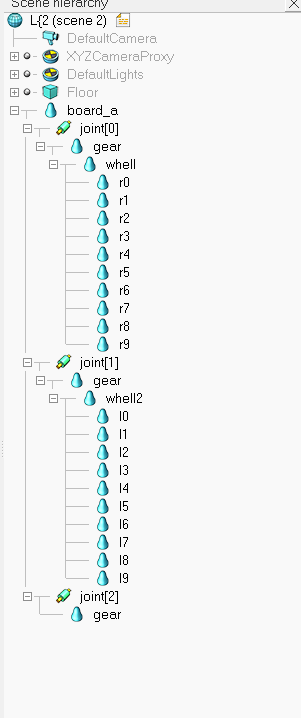
\includegraphics[width=15cm]{26}
\caption{\Large Operator interface during the WO  WO 期間的操作員介面}\label{fig.26}
\end{center}
\end{figure}


\section{ The engineering change order 工程變更單 }

\fontsize{12}{2.5pt}\sectionef 
 {As explained in the beginning of chapter 2 the Odoo management software considers
PLM mainly as a tool for tracking change and improvements. Its application module is
external to the normal flow of manufacturing but acts as an expansion to it. Its focal item
class is the Engineering Change Order (ECO). }\\[1pt]

\fontsize{12}{2.5pt}\sectionef  
{如第 2 章開頭所解釋的,Odoo 管理軟體考慮
PLM 主要作為追蹤變更和改進的工具。 其應用模組為
位於正常製造流程之外,但充當其擴展。 其重點項目
類別是工程變更單(ECO)。}\\[15pt]



\fontsize{12}{2.5pt}\sectionef 
 {An ECO is an item class that outlines the proposed changes to the product or the parts that
would be affected by the change. In other words, is a central information hub for everyone
associated with a given product. }\\[1pt]

\fontsize{12}{2.5pt}\sectionef  
{ECO 是一個項目類別,概述了產品或零件的建議變更
將受到該變化的影響。 換句話說,就是每個人的中央資訊中心
與給定產品相關聯。}\\[15pt]


\fontsize{12}{2.5pt}\sectionef 
 {The idea is to signal the need for change to a product item or a BOM item, hold the files
that are relevant to the change and apply the change or at least signal that the change has been
implemented, all while keeping the history of al the previous changes. All very useful in the
future and serve as a process to streamline product development and help improve
products/production.}\\[1pt]

\fontsize{12}{2.5pt}\sectionef  
{這個想法是表明需要更改產品項目或 BOM 項目,保存文件
與變更相關並應用變更或至少表示變更已經
實施,同時保留所有先前更改的歷史記錄。 一切都非常有用
未來並作為簡化產品開發並幫助改進的流程
產品/生產。}\\[15pt]



\begin{figure}[hbt!]
\begin{center}
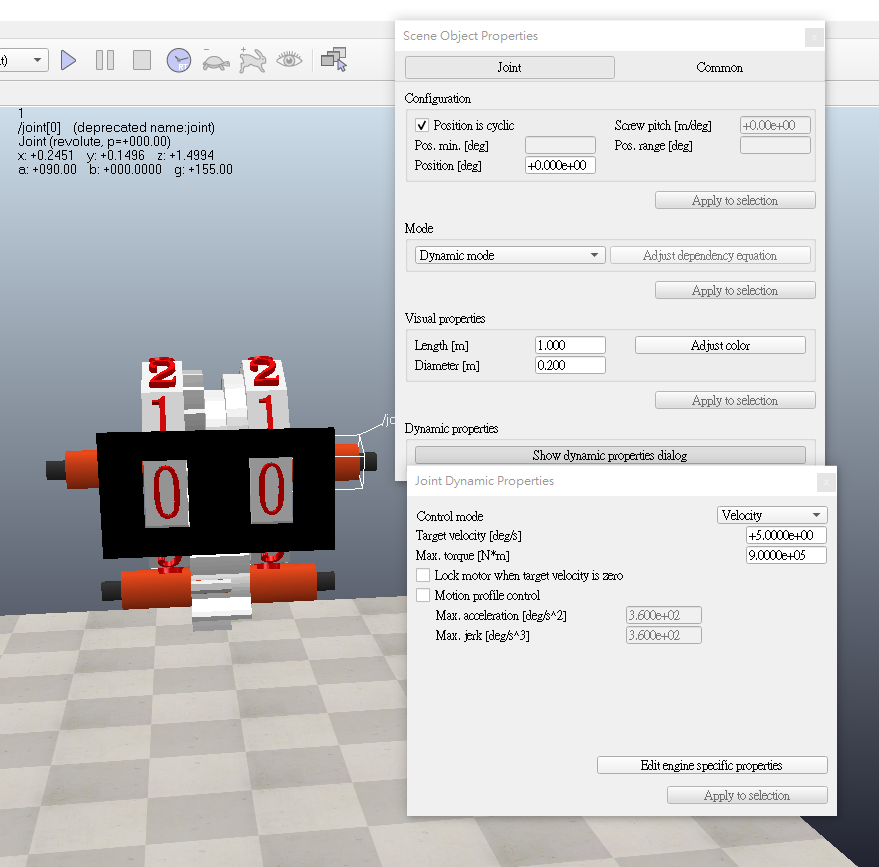
\includegraphics[width=15cm]{27}
\caption{\Large Simplified ECO function diagram 簡化的ECO功能圖}\label{fig.27}
\end{center}
\end{figure}
\newpage
%\pagenumbering{arabic} %設定頁號阿拉伯數字
\setcounter{page}{1}  %設定頁數
\section{Starting the simulation 開始模擬}
\subsection{Software option chosen for the simulation模擬所選擇的軟體選項}
\fontsize{14pt}{2.5pt}\sectionef {For this simulation, it has been decided that the best evaluation of the Odoo software would be through its online web-based service. The reasons for such choice instead of using the community edition of the software are as follows:}\\[1pt]
\fontsize{14pt}{5pt}\sectionef{對於這次模擬,我們決定通過Odoo軟體的在線網絡服務來進行最佳評估。選擇這種方式而不是使用軟體的社區版的原因如下:}\\[15pt]

\begin{itemize}
\item The practicality of using a web-based service as oppose to administrate a server locally or remotely. Although the community application was tested as part of the research for this work and has been judged to be a very beginner friendly server application the fact of the matter is that hosting a server is, on its own, a job that requires experience and knowledge. There has been a shift of the market regarding this sort of application towards product as a service and with good reason. At the time this thesis is being written the COVID-19 pandemic is forcing a lot of employees to work remotely and making clear to the market that IT is not a simple job and that a web service is an attractive option.
\item 相對於在本地或遠程管理服務器,使用基於Web的服務的實用性。儘管社區應用程式作為本項研究的一部分進行了測試,並且被判斷為非常適合初學者的服務器應用程式,但實際情況是,單獨運營服務器是一項需要經驗和知識的工作。市場對於這種類型的應用程式發生了轉變,向作為服務的產品轉移,並且有充分的理由。在撰寫本論文時,COVID-19大流行迫使許多員工遠程工作,並向市場表明IT工作並不簡單,而Web服務是一個具有吸引力的選擇。
\vspace{1cm}
\item Lack of official Odoo PLM application for the community edition of Odoo. Although there is a substantial repertoire of community made applications for the community edition of Odoo the organization, description, integration, and support of this applications are spotted at best. Rather than rely on applications that might not keep up with the main software it was decided that it would be a fairer to the platform evaluation if it was based on official applications. I.e. it would be very unproductive to slap together a free solution just to depend on luck regarding how it is supported on the future. PLM is the focus here, so this is an unnegotiable situation.
\item Odoo社區版缺乏官方的Odoo PLM應用程式。儘管有大量的由社區製作的Odoo社區版應用程式,但這些應用程式的組織、描述、整合和支持最多也只是達到及格水平。與其依賴可能跟不上主要軟體步伐的應用程式,我們決定,如果基於官方應用程式進行評估,將更公平地評估該平台。換句話說,將一個免費解決方案隨便拼湊在一起,僅僅依靠未來它如何得到支持,是非常不划算的。在這裡PLM是重點,因此這是一個不可妥協的情況。
\end{itemize}

\newpage
\fontsize{14pt}{2.5pt}\sectionef {At the time of writing this work, Odoo allows you to select one of its extra features like PLM and use it for free for an indefinite amount of time on their cloud hosted servers. This is a very attractive option if the only focus of this work was PLM and manufacturing. However, the MES aspect of this work is highly dependent of other applications of Odoo which means that there is very little that can be done. To this end the experiment was carried out in the trial version of Odoo enterprise which allow the user to use the system without storage or application limitations for a period of 14 days all hosted in Odoo cloud servers (Figure 17).}\\[1pt]
\fontsize{14pt}{5pt}\sectionef{在撰寫本文時,Odoo允許您在其雲端主機上選擇其額外功能之一,例如PLM,並無限期免費使用。如果本文的唯一焦點是PLM和製造業,那麼這是一個非常吸引人的選擇。然而,這項工作的MES方面高度依賴Odoo的其他應用程式,這意味著幾乎沒有什麼可以做。因此,實驗是在Odoo企業版的試用版本中進行的,該版本允許用戶在Odoo雲端服務器上使用系統,沒有存儲或應用程式限制,使用期限為14天(圖17)。}\\[15pt]
\subsection{Setings details that are relevant相關的設置細節}
\fontsize{14pt}{2.5pt}\sectionef {A few details regarding the settings of Odoo are relevant to the proper function of its manufacturing functionalities. Namely enabling work orders in the manufacturing settings is an obligatory step for proper use of both work order items, workcenter items and operation items.}\\[1pt]
\fontsize{14pt}{5pt}\sectionef{關於Odoo設置的一些細節與其製造功能的正確運作相關。具體而言,啟用製造設置中的工單是使用工單項目、工作中心項目和操作項目的正確步驟。}\\[15pt]
\fontsize{14pt}{2.5pt}\sectionef {An assumption made for this work is that this is a holdover of the ERP origins of the software because it is rather unintuitive to not have this setting enabled by default if you are going to use Odoo to make any serious control on manufacturing. Regardless as of Odoo enterprise v14 this option can be set in the Settings > Manufacturing > Operations > Work Orders (Figure 28).}\\[1pt]
\fontsize{14pt}{5pt}\sectionef{這項工作的假設是,這是該軟件的ERP起源的遺留問題,因為如果您要在Odoo上進行任何嚴肅的製造控制,那麼不將此設置默認啟用是相當不直觀的。儘管如此,從Odoo企業版v14開始,可以在「設置」>「製造」>「操作」>「工單」中設置此選項(圖28)。}\\[15pt]
\newpage

\begin{figure}[hbt!]
\begin{center}
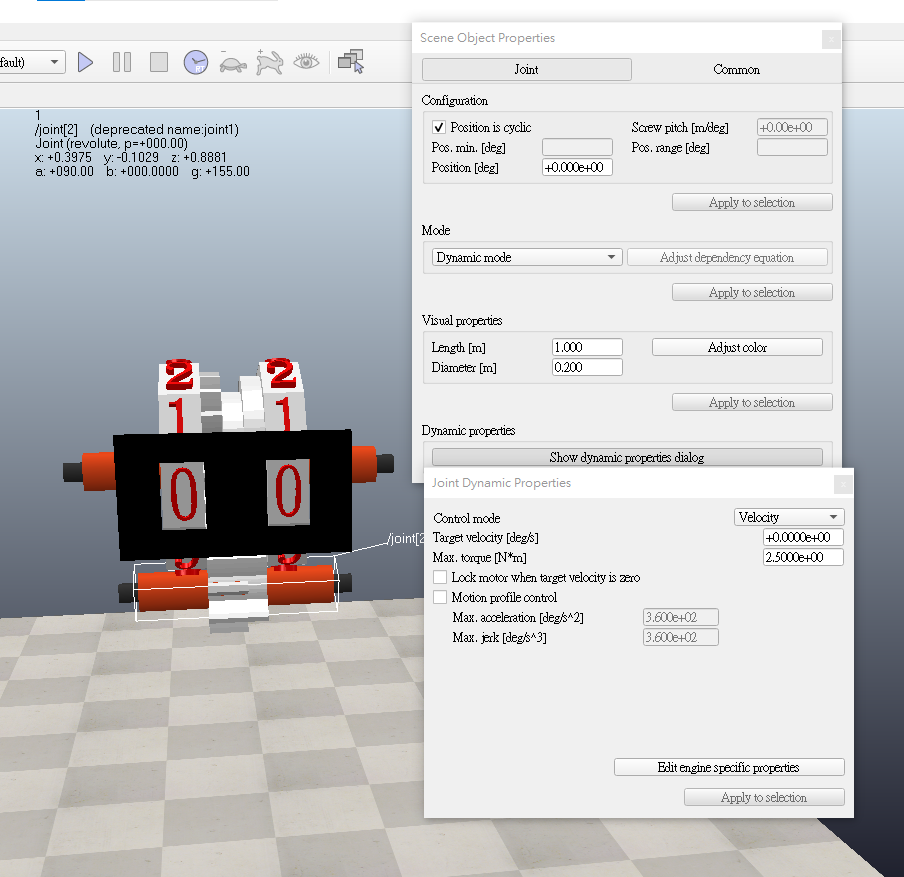
\includegraphics[width=15cm]{28}
\caption{\large Screenshot of the specific setting to be enabled\\特定設置的截圖}\label{fig.28}
\end{center}
\end{figure}

\section{Building the company structure 建立公司結構}
\subsection{User 使用者}

\fontsize{14pt}{2.5pt}\sectionef {Users are set and invited through the setting menu. It is possible to assign different levels of permissions regarding different aspects of the business operation. Messaging, permissions,approvals, responsibilities are all assigned into a user. This is very convenient and can fall within the category of virtual item class even if it has limited use in the scope of manufacturing. Their creation is not strictly necessary, the software would run just fine having just me as a user with full administrator credentials, but for this simulation, 5 users were created as listed below to represent different employees within the company. The following (Figure 29) is a screenshot of my user account item and its ‘Asses Rights’ followed by one of the fictional users being created for the company (Figure 30).}\\[1pt]
\fontsize{14pt}{5pt}\sectionef{使用者是透過設置選單設定並邀請的。可以針對業務運作的不同方面分配不同級別的權限。訊息、權限、批准、責任等都分配給使用者。這非常方便,即使在製造範圍內使用有限,也可以歸入虛擬項目類別。它們的創建不是絕對必要的,軟體只需我作為具有完整管理員權限的使用者即可正常運行,但為了這個模擬,已創建了5個使用者,如下所列,代表公司內的不同員工。下面(圖29)是我的使用者帳戶項目及其“評估權限”,接著是為公司創建的虛構使用者之一(圖30)的截圖。}\\[15pt]
\newpage

\begin{figure}[hbt!]
\begin{center}
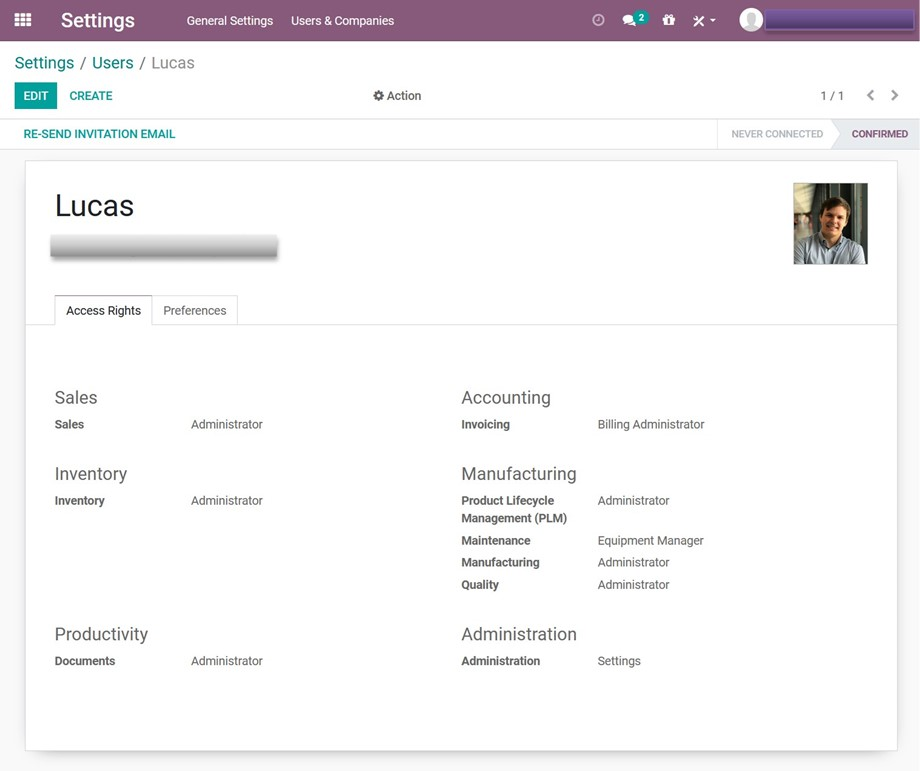
\includegraphics[width=15cm]{29}
\caption{\large  Screenshot of user account interface\\使用者帳戶介面截圖}\label{fig.29}
\end{center}
\end{figure}
\newpage

\begin{figure}[hbt!]
\begin{center}
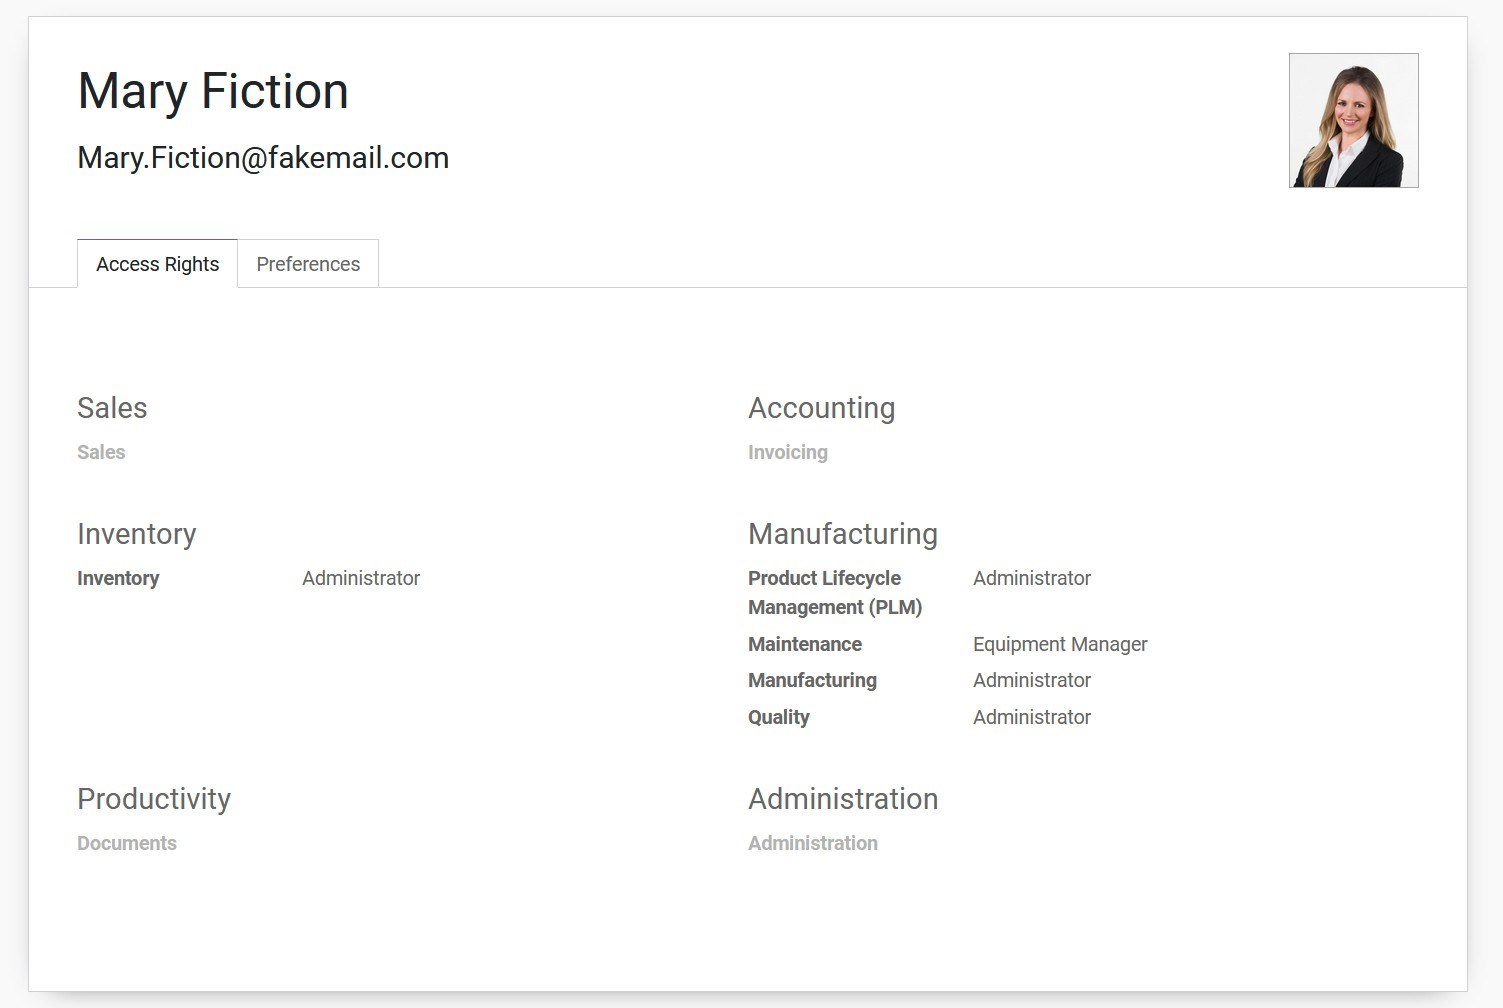
\includegraphics[width=15cm]{30}
\caption{\large  Screenshot of second user account interface\\第二個使用者帳戶介面截圖}\label{fig.30}
\end{center}
\end{figure}

\fontsize{14pt}{2.5pt}\sectionef {It is nice to point out how the two differ in access rights. Mary Fiction has been created in this example as an engineer and therefore most of her permissions are around the manufacturing procedure while she is denied access to other parts like Sales or Accounting.}\\[1pt]
\fontsize{14pt}{5pt}\sectionef{很好地指出這兩個使用者在訪問權限上的差異是不錯的。在這個例子中,Mary Fiction 被創建為一名工程師,因此她的大部分權限都圍繞著製造程序,同時她被拒絕訪問其他部分,如銷售或會計。}\\[15pt]

\subsection{Workcenters and Equipement 工作中心和設備}
\fontsize{14pt}{2.5pt}\sectionef {Workcenters are quite flexible within Odoo in the sense that they can be changed and expanded as needed. One could create the workcenters after creating the product items to allow for reorganization of the shop floor once you gained some perspective on what the products will be in the end. However, for most scenarios this seems unrealistic since the workcenters are more rigid structures in the real world - they don’t change as much as the products since they tend to hold heavy machinery.}\\[1pt]
\fontsize{14pt}{5pt}\sectionef{在Odoo中,工作中心在某種程度上非常靈活,可以根據需要進行更改和擴展。您可以在創建產品項目之後創建工作中心,以便在獲得一些關於最終產品的想法後重新組織車間。然而,對於大多數情況來說,這似乎不太現實,因為工作中心在現實世界中更加固定 - 它們不像產品那樣經常變化,因為它們往往安裝有重型機械。}\\[15pt]
\newpage

\fontsize{14pt}{2.5pt}\sectionef {In this simulation it was considered that the company already has 3 workcenters from the get-go and therefore the workcenters and machinery were created beforehand. This is more useful for possible readers interested in implementing Odoo as well as saving sometime.}\\[1pt]
\fontsize{14pt}{5pt}\sectionef{在這個模擬中,考慮到公司從一開始就已經擁有了3個工作中心,因此工作中心和機械是事先創建的。這對於有興趣實施Odoo的潛在讀者來說更加有用,也可以節省時間。}\\[15pt]

\fontsize{14pt}{2.5pt}\sectionef {We begin by creating the equipment we have. This is an item class that emphasizes in maintenance organization. The application responsible for managing equipment is the Maintenance App. The following image is an example of how Odoo portrays a 3D printer equipment item (Figure 31).}\\[1pt]
\fontsize{14pt}{5pt}\sectionef{我們首先創建我們擁有的設備。這是一個強調維護組織的項目類別。負責管理設備的應用程序是維護應用。下面的圖像是Odoo展示一個3D打印機設備項目的示例(圖31)。}\\[15pt]
\begin{figure}[hbt!]
\begin{center}
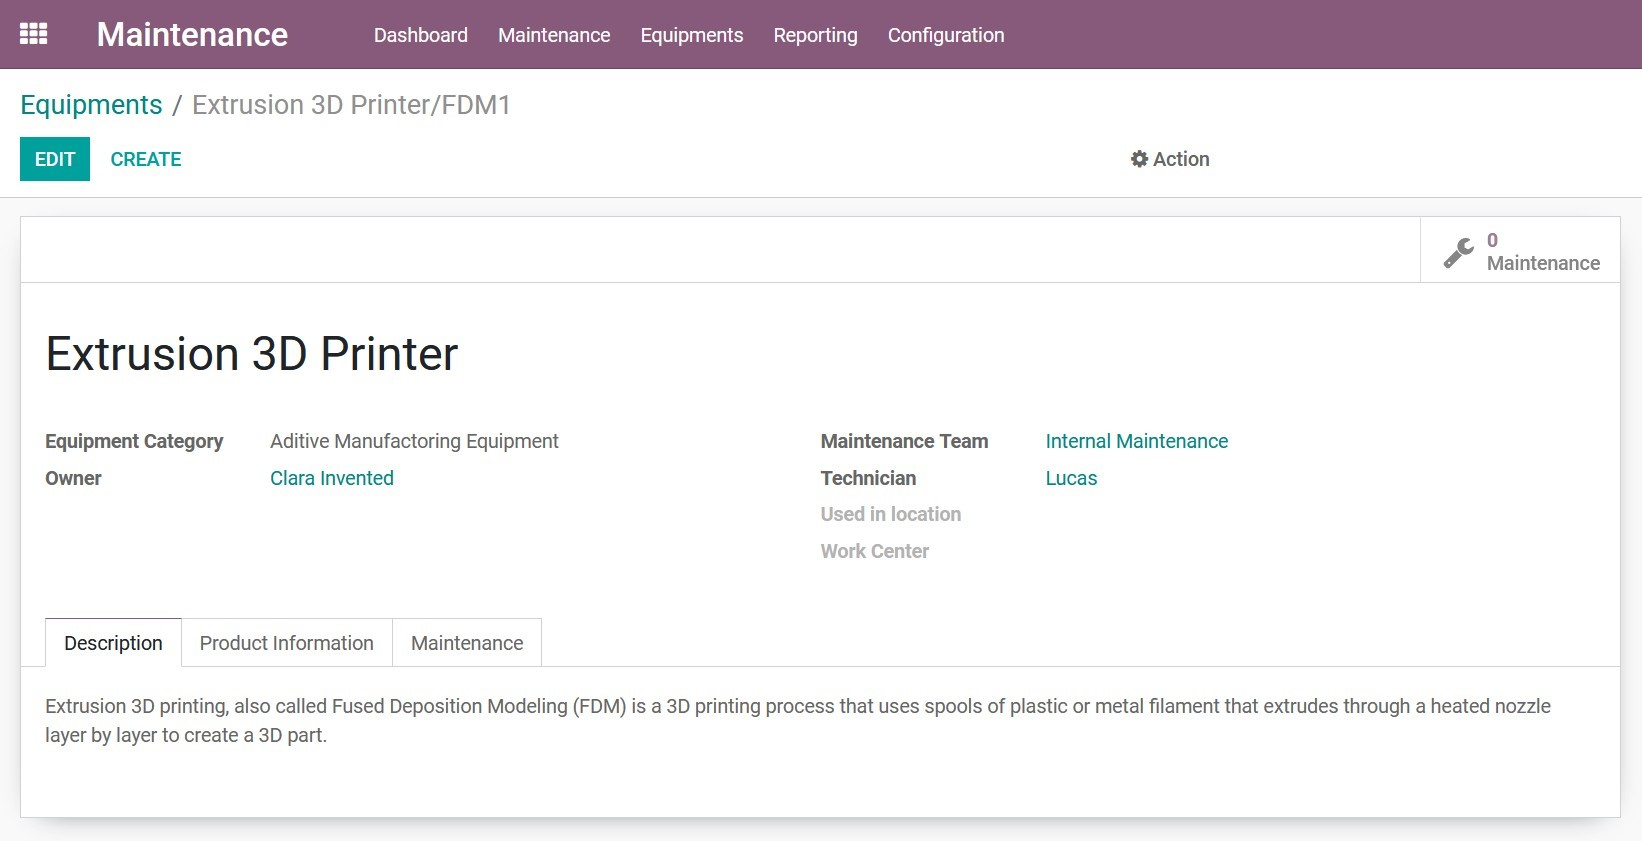
\includegraphics[width=15cm]{31}
\caption{\large  Odoo 3D printer equipment item\\Odoo 3D打印機設備項目}\label{fig.31}
\end{center}
\end{figure}

\fontsize{14pt}{2.5pt}\sectionef {In addition to this 3D printer the following equipment were created to be used throughout the development/production process (Figure 32):}\\[1pt]
\fontsize{14pt}{5pt}\sectionef{除了這台3D打印機外,還創建了以下設備,用於整個開發/生產過程}\\[15pt]
\fontsize{14pt}{5pt}\sectionef{(圖32):}\\[15pt]
\newpage

\begin{figure}[hbt!]
\begin{center}
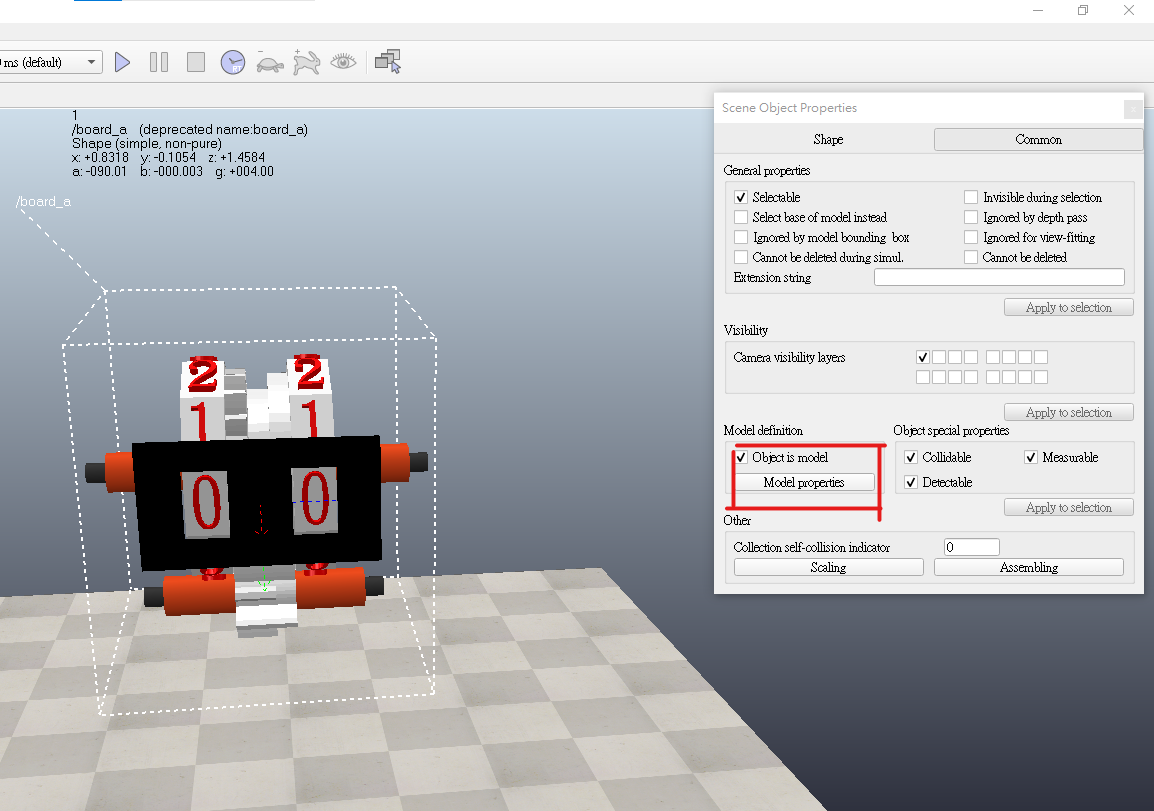
\includegraphics[width=15cm]{32}
\caption{\large  Overview of equipment items\\設備項目概觀}\label{fig.32}
\end{center}
\end{figure}

\fontsize{14pt}{2.5pt}\sectionef {This is where software limitations regarding PLM start to show. Although equipment items allow you some level of metadata (description text, responsible user, maintenance data and vendor). It does not allow for the uploading of files of any kind to be attached to the item class (machine manuals, reports etc). This is a substantial weakness, since file management is something quite unanimously considered a main aspect of PLM. This will be a recurring subject of this simulation since the number of Items that allow upload of files directly to them is limited in Odoo.}\\[1pt]
\fontsize{14pt}{5pt}\sectionef{這就是軟件在產品生命週期管理(PLM)方面開始顯示限制的地方。儘管設備項目允許一定程度的元數據(描述文字、負責用戶、維護數據和供應商),但它不允許上傳任何類型的文件附加到項目類別(機器手冊、報告等)。這是一個相當大的弱點,因為文件管理被普遍認為是PLM的主要方面之一。這將是這次模擬的一個反復出現的主題,因為在Odoo中,允許直接上傳文件的項目數量是有限的。}\\[15pt]
\fontsize{14pt}{2.5pt}\sectionef {Now that the equipment has been created, their workcenters can be created. It is interesting to remember that the main use of the workcenter item is management of time and cost per hour. The idea is that equipment assigned to a WC should not be used at the same time and that ideally equipment that have widely different running costs should also be in different workcenters to allow for better time/cost tracking.}\\[1pt]
\fontsize{14pt}{5pt}\sectionef{現在設備已經創建,它們的工作中心可以被建立了。值得一提的是,工作中心項目的主要用途是按小時管理時間和成本。這個想法是分配給工作中心的設備不應該同時使用,而且理想情況下,具有截然不同的運行成本的設備也應該位於不同的工作中心,以便更好地跟蹤時間/成本。}\\[15pt]
\fontsize{14pt}{2.5pt}\sectionef {The following (Figure 33) is a an example of a workcenter item made to represent the prototyping station that is used throughout the development of the product.}\\[1pt]
\fontsize{14pt}{5pt}\sectionef{以下(圖33)是一個工作中心項目的示例,用來代表在產品開發過程中使用的原型製作站。}\\[15pt]
\newpage

\begin{figure}[hbt!]
\begin{center}
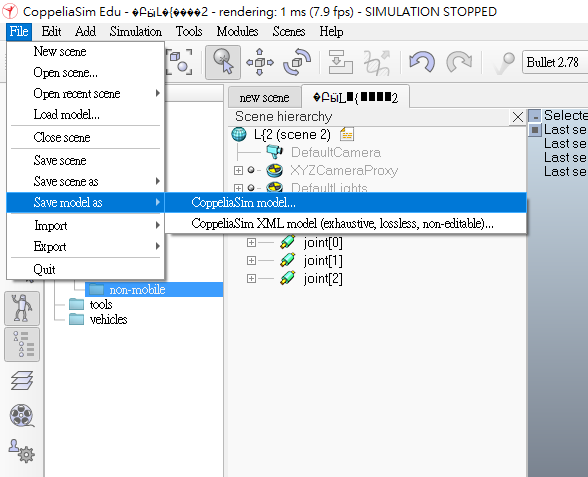
\includegraphics[width=15cm]{33}
\caption{\large  Odoo Prototyping Station item representation 1\\Odoo原型製作站項目表示1}\label{fig.33}
\end{center}
\end{figure}

\fontsize{14pt}{2.5pt}\sectionef {The reader will notice that this station (Figure 34) is where the 3D printers and CNC machine are located. Usually these machines would be separated in singular workcenters because of difference in operation costs and because they are for the most part independent however for the sake of this simulation this has been considered representative enough.}\\[1pt]
\fontsize{14pt}{5pt}\sectionef{讀者會注意到這個站點(圖34)是3D打印機和CNC機床的所在地。通常,由於操作成本的差異以及它們在很大程度上是獨立的,這些機器會被分開放置在不同的工作中心中。然而,出於模擬的目的,這被認為足夠具有代表性}\\[15pt]
\newpage

\begin{figure}[hbt!]
\begin{center}
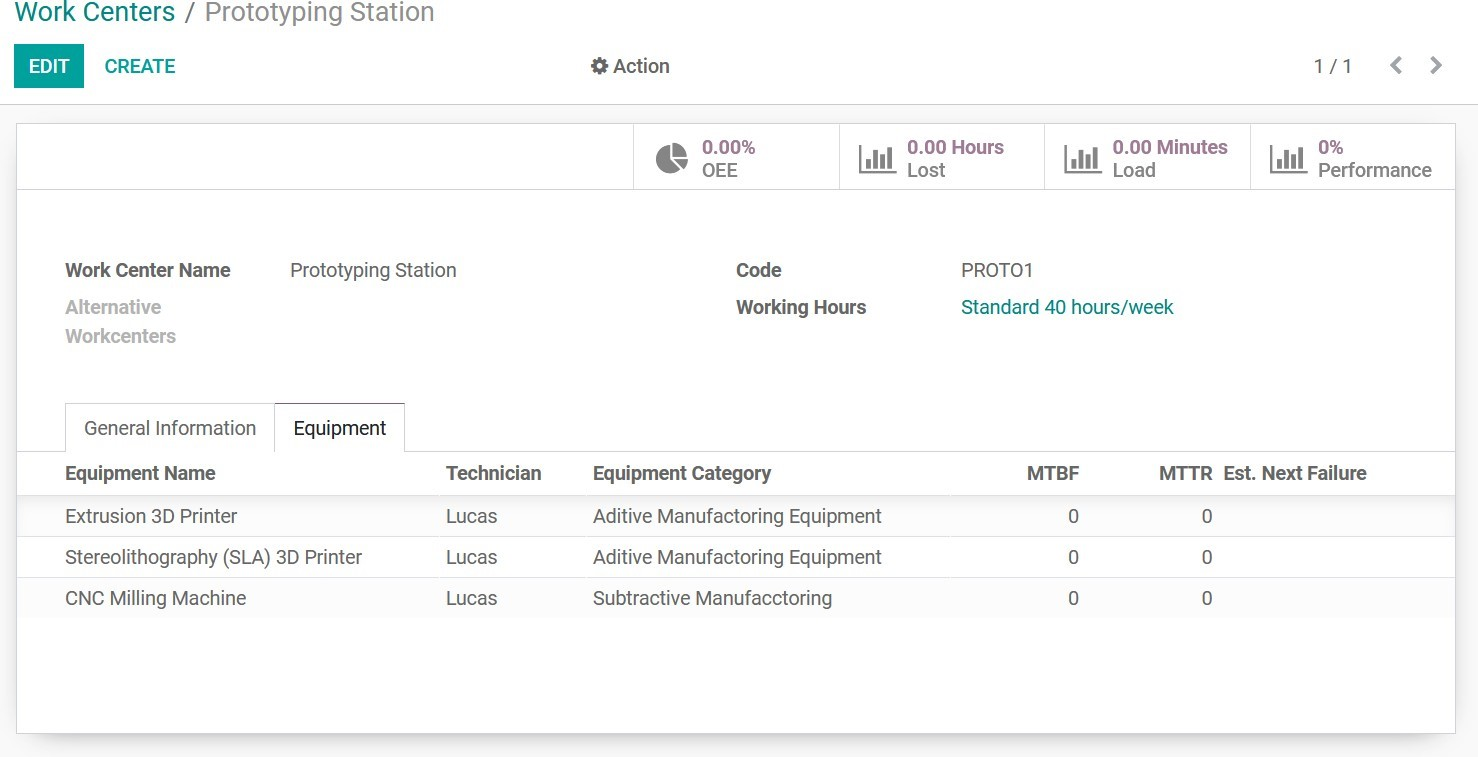
\includegraphics[width=15cm]{34}
\caption{\large  Prototyping Station item representation 2\\原型製作站項目表示2}\label{fig.34}
\end{center}
\end{figure}

\fontsize{14pt}{2.5pt}\sectionef {The following (Figure 35) workcenters have been also created for the simulation and filed with the necessary equipment:}\\[1pt]
\fontsize{14pt}{5pt}\sectionef{以下(圖35)工作中心也已經為模擬創建並填入必要的設備:}\\[15pt]

\begin{figure}[hbt!]
\begin{center}
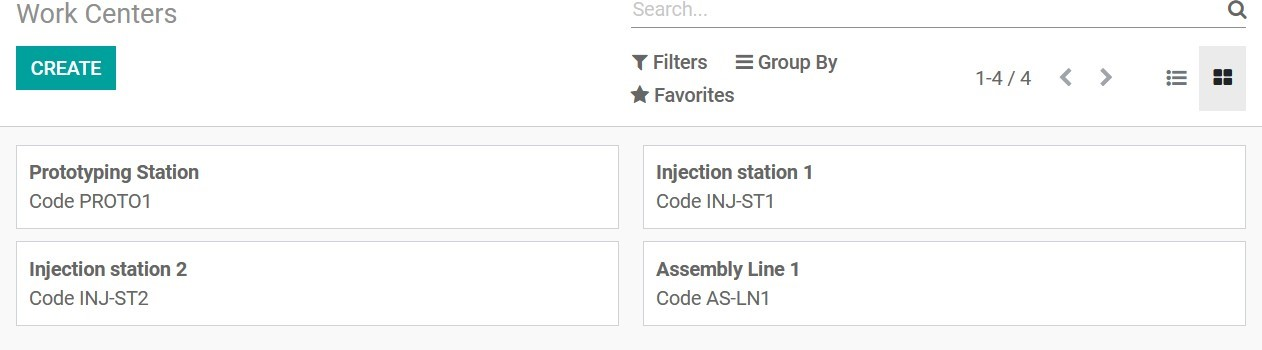
\includegraphics[width=15cm]{35}
\caption{\large  Overview of Workcenter items\\工作中心項目概覽}\label{fig.35}
\end{center}
\end{figure}
%\newpage
\pagenumbering{arabic} %設定頁號阿拉伯數字
\setcounter{page}{1}  %設定頁數
\fontsize{12pt}{2.5pt}\sectionef
\section{Development 發展}
\fontsize{12}{2.5pt}\selectfont {Now that the basic structure of the company has been recreated in the software, it is
possible to commence the simulation process. At first, the focus is on the development aspect
of a brand new product using Odoo (Figure 9) most noticeably, since this is the company first
product to be created, a possible use of Odoo for organizing prototyping procedure is
evaluated. This include the path from idea to design and prototype production. Then once the
product has reached an acceptable result as a prototype, the work regarding the development
of the production process will take place. The product development is considered successful
once an official production run is done.}\\[1pt]

\fontsize{12}{2.5pt}\selectfont {現在公司的基本結構已經在軟體中重新創建了,
可以開始模擬過程。首先,重點是發展方面最引人注目的是使用 Odoo 的全新產品(圖 9),因為這是該公司的第一個產品要創建的產品,Odoo 組織原型製作過程的可能用途是評價。這包括從想法到設計和原型生產的路徑。然後一旦產品作為原型已達到可接受的結果,有關開發的工作將發生生產過程。產品開發被認為是成功的一旦正式生產運作完成。}\\[1pt]

\section{. Idea - design - product prototype 創意-設計-產品原型}
\fontsize{12}{2.5pt}\selectfont {As explained in (Chapter 4) the idea for the product has already been stablished and initial
design characteristics and basic product research have already been carried out. This is
representative of an actual implementation of the Odoo software in the real world because
although Odoo have good project management and communication applications, those are
external to the inventory and manufacturing applications and, more importantly, share no
integration with the engineering design CAD software. In this simulation, the idea has been
put to paper and have been turned into a CAD design using the Solidworks software
generating a CAD file locally stored in the engineer computer}\\[1pt]
\fontsize{12}{2.5pt}\selectfont {如同(第 4 章)中所解釋的,產品的想法已經確定並初步確定
設計特點和產品基礎研究已經進行。這是
代表 Odoo 軟體在現實世界中的實際實施,因為
儘管 Odoo 有良好的專案管理和通訊應用程序,但這些應用程式
庫存和製造應用程式之外,更重要的是,不共享
與工程設計CAD軟體整合。在這個模擬中,這個想法是
使用 Solidworks 軟體將其寫在紙上並轉換為 CAD 設計
產生本機儲存在工程師電腦中的 CAD 文件}\\[1pt]
\begin{figure}[hbt!]
\begin{center}
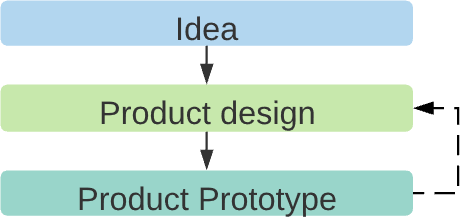
\includegraphics[width=8cm]{36}
\caption{\Large Sectioned diagram regarding product development  產品開發剖面圖}\label{fig.36}
\end{center}
\end{figure}
\fontsize{12}{2.5pt}\selectfont {It is at this point that the utilization of the Odoo software can officially take place. The
first step is to understand what the subject of production is as far as product items are
concerned. There are two takes in how to do this:
▪ The first is to consider the prototype an early revision of the final product, that is
the prototype item created in Odoo would be the same as the final product item
with revisions been carried out during development. That would be the
recommended if the prototype is achieved by identical means to the ones used in
the final production. An example of this approach would be if the product is
simple enough that product and production aspects of development can be carried
out together.
▪ The second one is to consider the prototype as a separate item from the final
product - this is the path was taken in this simulation. The main reason for this
decision was that the ways in which our prototype production were carried out
differed from the final production since 3D printing was used for the prototypes.
Starting from the root, a product item called PROTO Alpha Case (Figure 37) was created
(Alpha Case being the name of the product). From this point on we will refer to prototype
products as ‘proto item’. As we can see, this allows for a nice representation of the proto
item. Since it is a prototype, it will not be marked as something that can be sold or purchased,
and sales price will be set to 0 since it is unimportant. This proto item will be used to connect
the different aspects of its development but for now it is left alone.}\\[1pt]

\fontsize{12}{2.5pt}\selectfont {此時即可正式使用 Odoo 軟體。這第一步是了解生產的主題是什麼,就產品項目而言擔心的。如何做到這一點有兩種做法:▪ 首先是將原型視為最終產品的早期修訂版,即在 Odoo 中創建的原型項目將與最終產品項目相同在開發過程中進行了修改。那將是如果原型是透過與中使用的相同的方式實現的,則推薦最終的製作。這種方法的一個例子是,如果產品是夠簡單,可以進行產品和生產的開發一起出去。▪ 第二個是將原型視為獨立於最終產品的單獨項目產品 - 這是本次模擬中所採取的路徑。造成這種情況的主要原因決定是我們的原型生產的方式由於原型使用了 3D 列印,因此與最終產品有所不同。從根開始,創建了一個名為 PROTO Alpha Case(圖 37)的產品項(Alpha Case 是產品的名稱)。從現在開始我們將參考原型產品作為「原型項目」。正如我們所看到的,這可以很好地表示原型物品。由於它是原型,因不會標記為可以出售或購買的東西,銷售價格將設定為 0,因為它不重要。此原型項目將用於連接其發展的不同方面,但目前它被擱置了。}\\[1pt]
\begin{figure}[hbt!]
\begin{center}
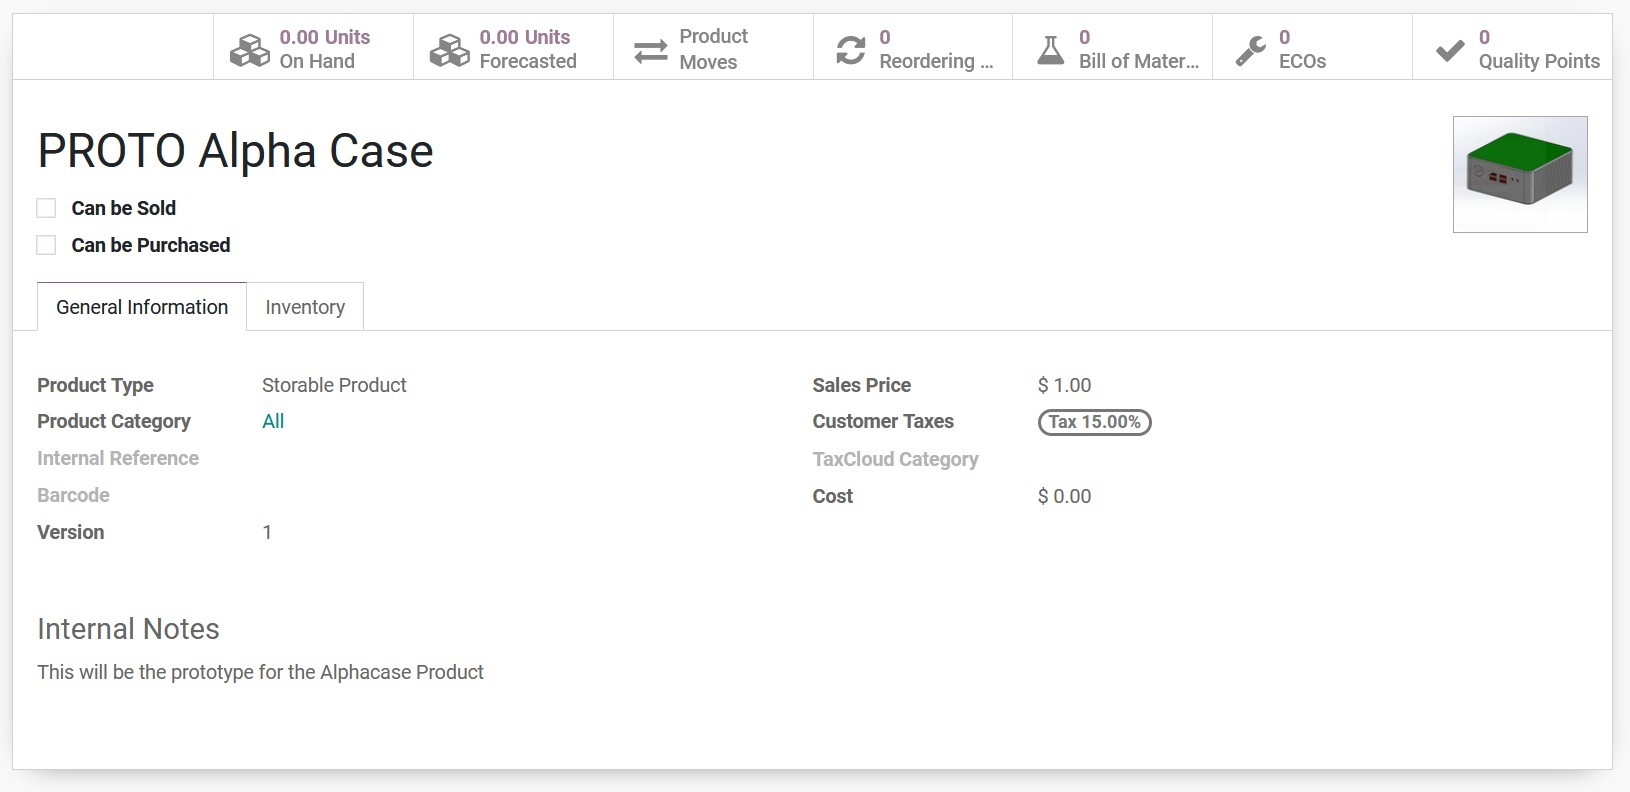
\includegraphics[width=10cm]{37}
\caption{\Large Image of the prototype product item  原型產品項目的圖像圖}\label{fig.37}
\end{center}
\end{figure}
\fontsize{12}{2.5pt}\selectfont {As we have previously stablished in chapter 3, the product will consist of 3 pieces Part A, Part B and Part C. These need to be prototyped and created as products as well so that they can be added to the bill of materials of the PROTO Alpha Case. Finally, it was decided to use specific plastic filaments (see section 4.1.1) for the 3D printing of PROTO Part A and PROTO Part B and C and these need to be added as products as well (Figure 38).}\\[1pt]

\fontsize{12}{2.5pt}\selectfont {正如我們之前在第 3 章中所確定的,該產品將由 3 部分組成:A 部分、B 部分和 C 部分。這些也需要進行原型設計並創建為產品,以便可以將它們添加到 PROTO 的物料清單中阿爾法案例。最後,決定使用特定的塑膠絲(請參閱第 4.1.1 節)來 3D 列印原型 A 部分以及原型 B 和 C 部分,並且這些也需要作為產品添加(圖 38)。}\\[1pt]
\begin{figure}[hbt!]
\begin{center}
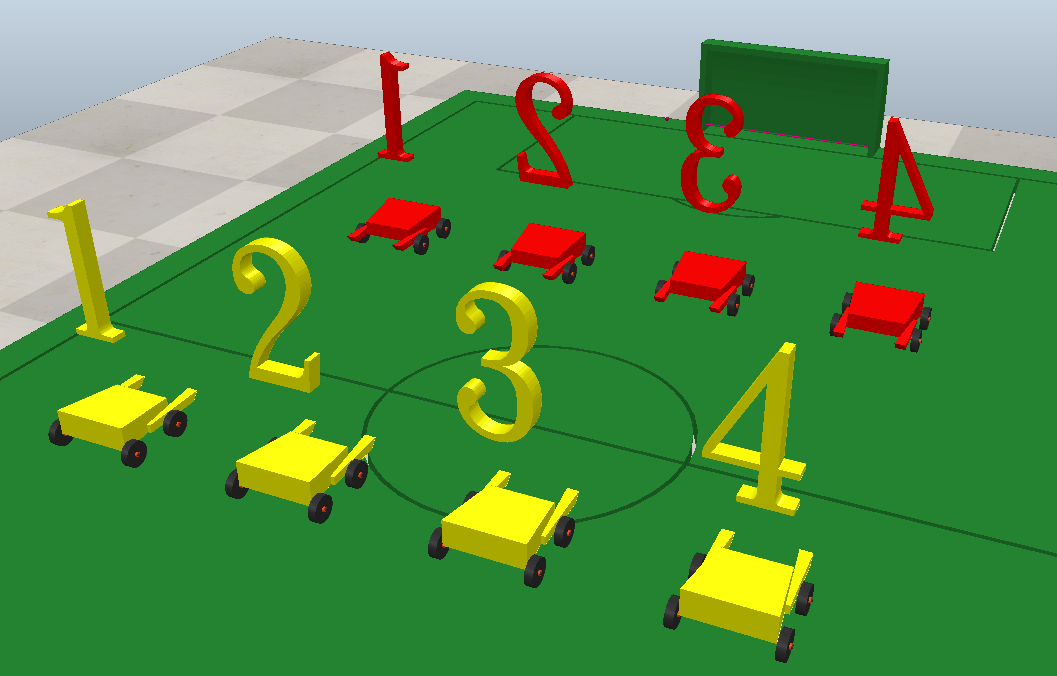
\includegraphics[width=10cm]{38}
\caption{\Large Overview of Product class items for prototype 原型產品類別項目概述}\label{fig.38}
\end{center}
\end{figure}
\fontsize{12}{2.5pt}\selectfont {At this point, the relevant product items for the prototyping of the Alpha Case were finished, which makes possible the creation of the its relevant BOMs. There are 3 of them and they follow the structure in (Figure 39)}\\[1pt]

\fontsize{12}{2.5pt}\selectfont {至此,Alpha Case原型製作的相關產品項目已經完成,可以創造其相關的BOM。其中有 3 個,它們遵循(圖 39)中的結構}\\[1pt]
\newpage
\begin{figure}[hbt!]
\begin{center}
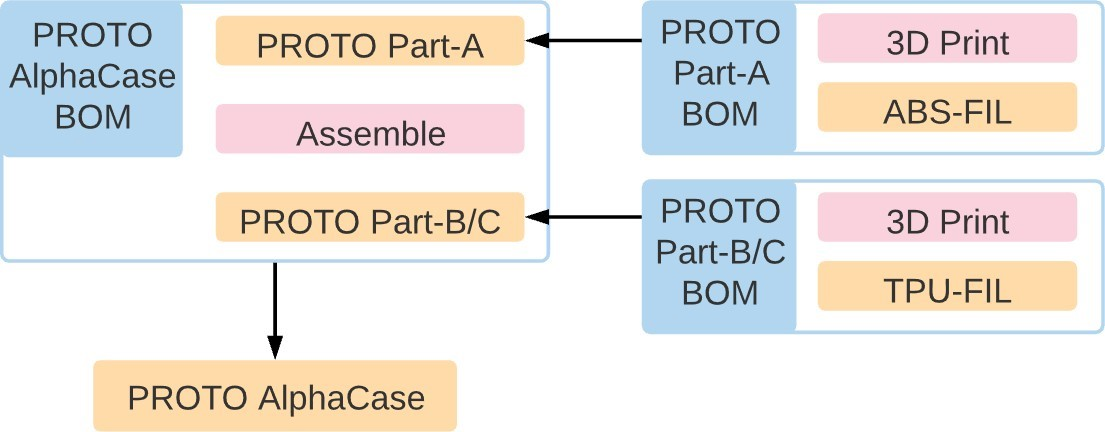
\includegraphics[width=10cm]{39}
\caption{\Large BOM diagrams for prototyping  用於原型設計的 BOM 圖}\label{fig.39}
\end{center}
\end{figure}

\fontsize{12}{2.5pt}\selectfont {Something worth mentioning is that Odoo used the kit option (Figure 40) on the item to infer that this product is a component of another product. This is very interesting because it automatically creates dependencies between the product items for production}\\[1pt]

\fontsize{12}{2.5pt}\selectfont {值得一提的是,Odoo 在該商品上使用了套件選項(圖 40)來推斷該產品是另一個產品的組件。這非常有趣,因為它會自動在生產的產品項目之間建立依賴關係。}\\[1pt]
\begin{figure}[hbt!]
\begin{center}
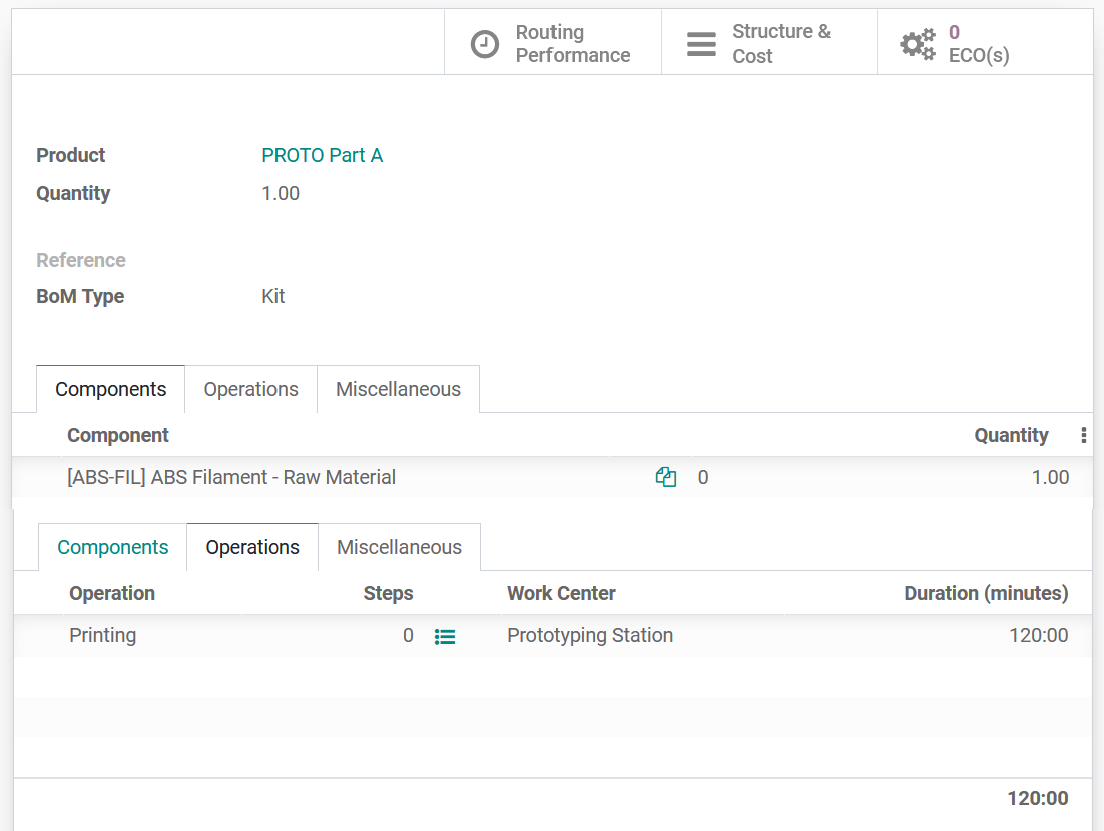
\includegraphics[width=15cm]{40}
\caption{\Large Image of the prototype product BOM (Part-A)  原型產品 BOM(A 部分)}\label{fig.40}
\end{center}
\end{figure}
\fontsize{12}{2.5pt}\selectfont {As the reader can see (Figure 41), while making the BOMs it is simple to create the specific operation items necessary for the manufacturing procedure and specify its work center. One of the best functionalities regarding MES in Odoo is the ability to track the time of operations based on default duration. This can be dynamically changed based on tracked time or set manually. It is also in the operation item that we can add instruction files for the operation. Even though it is limited to PDF text or a link to a google slides file, this is one of the few opportunities presented by Odoo for file management connected directly to an item.}\\[1pt]


\fontsize{12}{2.5pt}\selectfont {如讀者所見(圖 41),在製作 BOM 時,可以輕鬆創建製造過程所需的特定操作項目並指定其工作中心。 Odoo 中 MES 的最佳功能之一是能夠根據預設持續時間追蹤操作時間。這可以根據追蹤時間動態更改或手動設定。也是在操作項中我們可以新增操作的指令檔。儘管它僅限於 PDF 文字或 Google 幻燈片文件的鏈接,但這也是 Odoo 為直接連接到專案的文件管理提供的少數機會之一。}\\[1pt]
\begin{figure}[hbt!]
\begin{center}
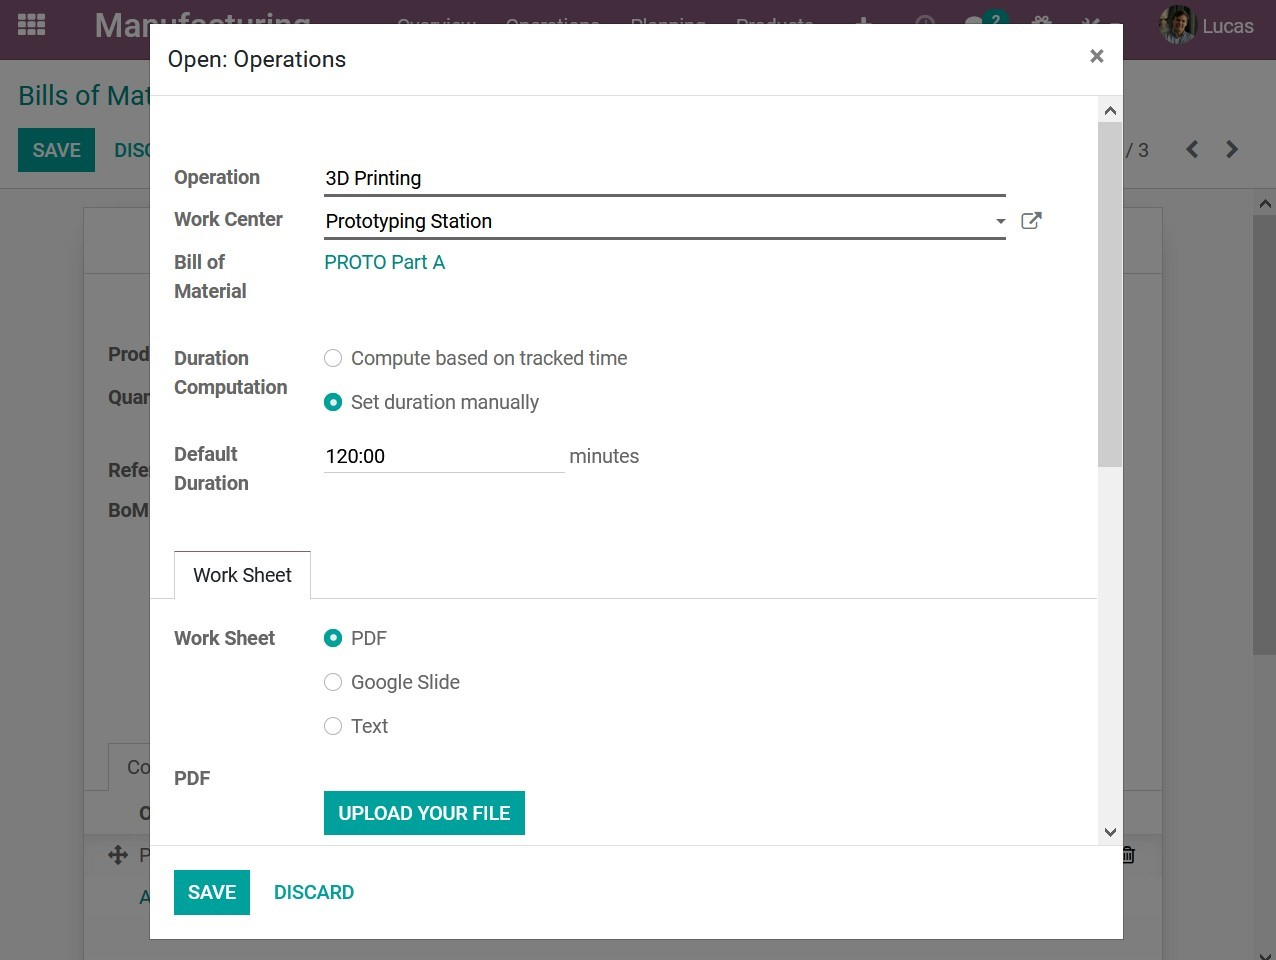
\includegraphics[width=10cm]{41}
\caption{\Large Image of the prototype product BOM (Part-A)  原型產品 BOM(A 部分)}\label{fig.41}
\end{center}
\end{figure}

\begin{figure}[hbt!]
\begin{center}
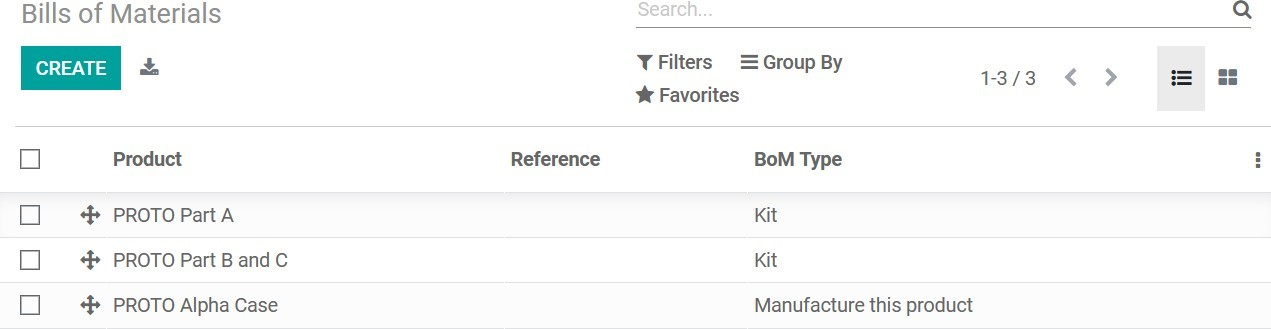
\includegraphics[width=10cm]{42}
\caption{\Large Overview of BOMs created for prototyping  為原型設計創建的 BOM 概述}\label{fig.42}
\end{center}
\end{figure}
\fontsize{12}{2.5pt}\selectfont {Speaking of this lack of upload opportunities, we can notice that while making the product item there was no way to directly upload files regarding the product to the item. In our case, we have the CAD files regarding the parts that we are prototyping, to not be able to upload these files in any way would be a complete failure from a PLM perspective. Thankfully there is a workaround. As explained in section 5.1.3.5, the ECO is an item that is linked to either product items or BOMs and allow uploaded files to be attached to it. It is a minor workaround but basically means that if we want to upload our CAD files to the items in any significative manner, we need to emit an ECO even if there is no “change” being made.}\\[1pt]

\fontsize{12}{2.5pt}\selectfont {說到缺乏上傳機會,我們可以注意到,在製作產品項目時,無法直接將有關產品的文件上傳到該項目。在我們的例子中,我們擁有與我們正在製作原型的零件相關的 CAD 文件,從 PLM 的角度來看,如果無法以任何方式上傳這些文件,那將是徹底的失敗。值得慶幸的是,有一個解決方法。如第 5.1.3.5 節所述,ECO 是連結到產品項目或 BOM 的項目,並允許將上傳的檔案附加到其上。這是一個較小的解決方法,但基本上意味著,如果我們想以任何有意義的方式將 CAD 檔案上傳到項目,即使沒有進行“更改”,我們也需要發出 ECO。}\\[1pt]
\newpage
\begin{figure}[hbt!]
\begin{center}
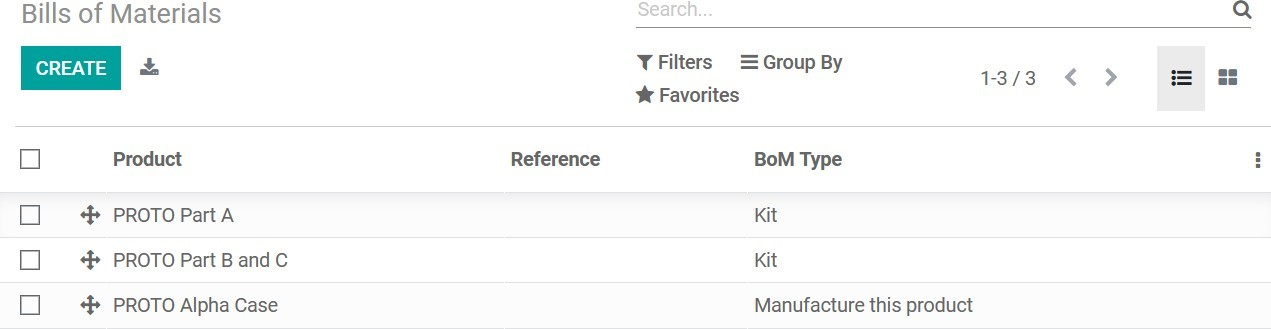
\includegraphics[width=10cm]{42}
\caption{\Large Overview of BOMs created for prototyping  為原型設計創建的 BOM 概述}\label{fig.42}
\end{center}
\end{figure}
\fontsize{12}{2.5pt}\selectfont {Speaking of this lack of upload opportunities, we can notice that while making the product item there was no way to directly upload files regarding the product to the item. In our case, we have the CAD files regarding the parts that we are prototyping, to not be able to upload these files in any way would be a complete failure from a PLM perspective. Thankfully there is a workaround. As explained in section 5.1.3.5, the ECO is an item that is linked to either product items or BOMs and allow uploaded files to be attached to it. It is a minor workaround but basically means that if we want to upload our CAD files to the items in any significative manner, we need to emit an ECO even if there is no “change” being made.}\\[1pt]

\fontsize{12}{2.5pt}\selectfont {說到缺乏上傳機會,我們可以注意到,在製作產品項目時,無法直接將有關產品的文件上傳到該項目。在我們的例子中,我們擁有與我們正在製作原型的零件相關的 CAD 文件,從 PLM 的角度來看,如果無法以任何方式上傳這些文件,那將是徹底的失敗。值得慶幸的是,有一個解決方法。如第 5.1.3.5 節所述,ECO 是連結到產品項目或 BOM 的項目,並允許將上傳的檔案附加到其上。這是一個較小的解決方法,但基本上意味著,如果我們想以任何有意義的方式將 CAD 檔案上傳到項目,即使沒有進行“更改”,我們也需要發出 ECO。}\\[1pt]
\newpage
\begin{figure}[hbt!]
\begin{center}
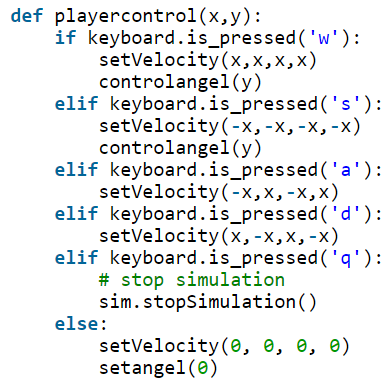
\includegraphics[width=10cm]{43}
\caption{\Large ECO example  生態範例}\label{fig.43}
\end{center}
\end{figure}

\fontsize{12}{2.5pt}\selectfont {It can only be assumed that this was part of Odoo’s team strategy to implement PLM as an external application in its ERP base. It is reasonable, but still, this is one of the few aspects of this software interface that is not as straightforward. It is an extremely valuable feature, but it is somewhat hidden. The documents icon appears in the top right corner (Figure 43) only after the ECO is created and saved.}\\[1pt]


\fontsize{12}{2.5pt}\selectfont {只能假設這是 Odoo 團隊策略的一部分,即將 PLM 作為其 ERP 基礎中的外部應用程式實施。這是合理的,但這仍然是該軟體介面中少數幾個不那麼簡單的方面之一。這是一個非常有價值的功能,但它有些隱藏。僅在建立並儲存 ECO 後,文件圖示才會出現在右上角(圖 43)。}\\[1pt]
\newpage
\begin{figure}[hbt!]
\begin{center}
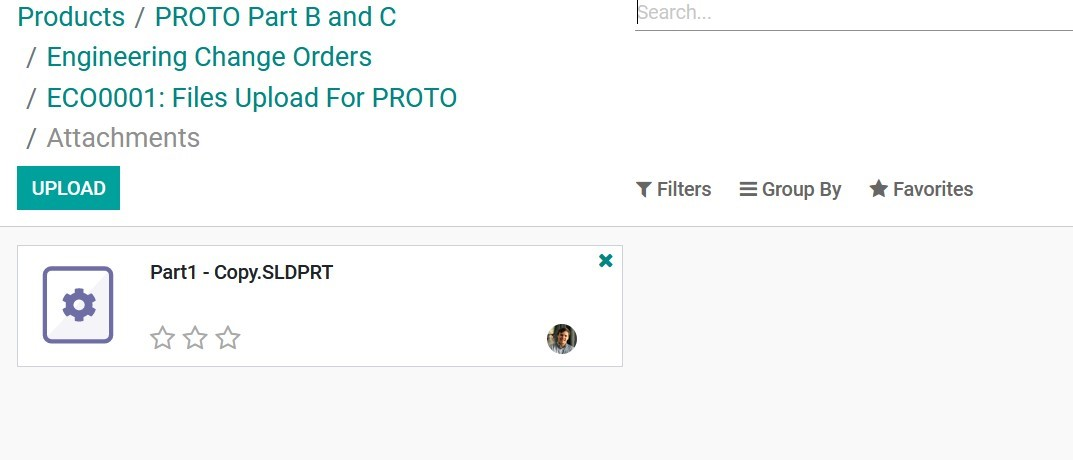
\includegraphics[width=10cm]{44}
\caption{\Large Overview of attached files to ECO ECO 附文件概述}\label{fig.44}
\end{center}
\end{figure}
\fontsize{12}{2.5pt}\selectfont {Since there is no direct integration between Odoo and the CAD software, uploading the file do not cause any automatic change to the product metadata. This is not ideal from the PLM perspective, still, it is a well implemented feature. By allowing product items to link directly to not only one existing ECO but to the list of all ECOs ever applied to the item, the software does well in tracking version control and development.

Something interesting that can be done for the sake of process control is adding quality control points to operations. This allows the responsible personnel to give feedback during the production regarding concerning points to the engineering team. In our case, we are concerned about 3D printing warping. This is something that happens when temperature varies to much during the 3D printing procedure. To this end a Quality Control Point item will be created (Figure 45) that will enquire with the operator to check if there is warping in the piece and mark pass or fail.
}\\[1pt]

\fontsize{12}{2.5pt}\selectfont {由於 Odoo 和 CAD 軟體之間沒有直接集成,因此上傳檔案不會導致產品元資料發生任何自動變更。從 PLM 的角度來看,這並不理想,但它仍然是實施良好的功能。透過允許產品項目不僅直接連結到一個現有的 ECO,而且連結到曾經應用於該項目的所有 ECO 的列表,該軟體在追蹤版本控制和開發方面表現良好。

為了過程控制可以做的一些有趣的事情是在操作中添加品質控制點。這使得負責人員可以在生產過程中向工程團隊提供有關要點的回饋。在我們的案例中,我們擔心 3D 列印翹曲。這是 3D 列印過程中溫度變化過大時會發生的情況。為此,將建立一個品質控制點專案(圖 45),該專案將詢問操作員以檢查工件是否存在翹曲並標記為通過或失敗。}\\[1pt]
\newpage
\begin{figure}[hbt!]
\begin{center}
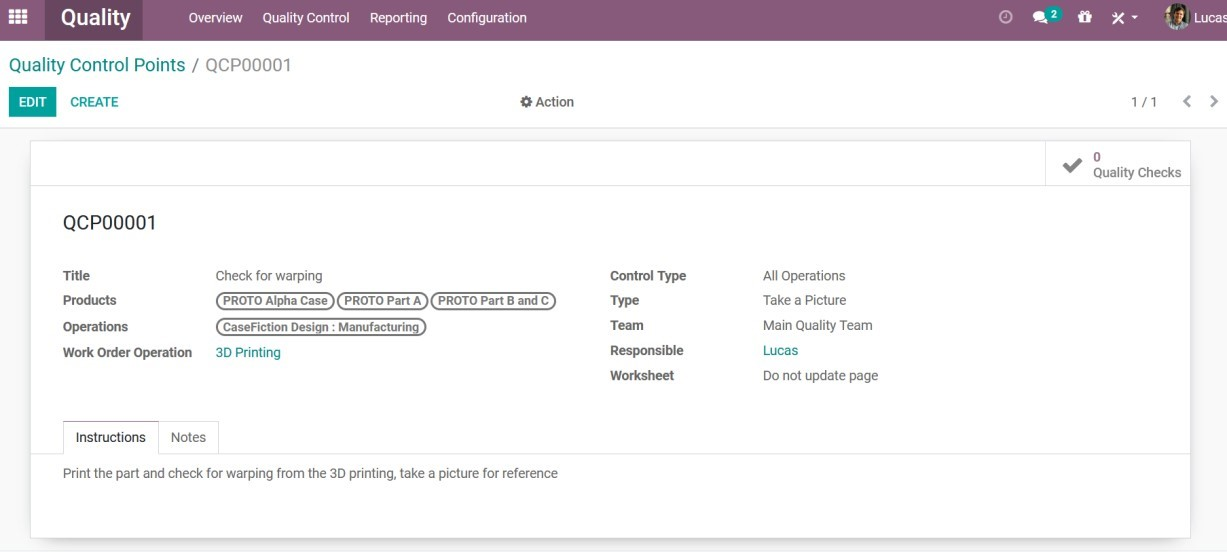
\includegraphics[width=10cm]{45}
\caption{\Large Quality Control Point item for the prototype production 原型生產的品質控制點項目}\label{fig.45}
\end{center}
\end{figure}
\fontsize{12}{2.5pt}\selectfont {The last step of a prototype cycle would be the production of prototypes for testing and evaluation. Production is something quite straightforward in Odoo and really the point where everything we have done before come together. The metadata and the items that have been created allow us to start the Manufacturing Order (MO) (Figure 46). This, in turn, pull the necessary workorders from the operations and components listed in the BOM. The workorders appear for manufacturing operators and production can commence/be tracked.
}\\[1pt]

\fontsize{12}{2.5pt}\selectfont {原型週期的最後一步是生產用於測試和評估的原型。在 Odoo 中,製作是相當簡單的事情,也是我們之前所做的一切都匯集在一起的地方。已建立的元資料和項目使我們能夠啟動製造訂單 (MO)(圖 46)。這反過來又從 BOM 中列出的操作和組件中提取必要的工作訂單。工作訂單會出現給製造操作員,並且可以開始/追蹤生產。}\\[1pt]
\newpage
\begin{figure}[hbt!]
\begin{center}
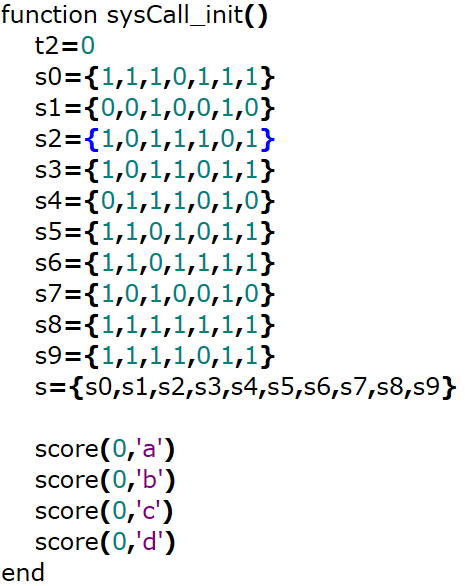
\includegraphics[width=10cm]{46}
\caption{\Large Depiction of the manufacturing order 製造訂單的描述}\label{fig.46}
\end{center}
\end{figure}
\fontsize{12}{2.5pt}\selectfont {For the most part this operation is very well automated and clear. There are however a few problems that are result of structural changes from Odoo V13 to Odoo V14. For a long time, the software ordered the operations to be carried out using an extra item class called ‘Route’. These were a fundamental part of how the product moved within the inventory and manufacturing, but for some reason, was dropped in the manufacturing aspect of the new version in favor of a simplified sequence data built into the BOM. As of the writing of this work, there have been reports of problems and confusions regarding how that works, which are aggravated by the fact that material explaining the use of this functionality are either nonexistent or still referencing old versions of the software (in which ‘routes’ are still in use).

The avid reader will notice in Figure 47 that the order in which operations are being made available are not in the correct sequence. This is due to exactly this problem and for now the
 
only solution is to count on the awareness of the operators regarding the order of production or manually scheduling the operations in the plan tab. During the period of research for this work (before Odoo V14) familiarization experiments were made in which there were no problem of this nature. In addition, there are examples online even from Odoo website demonstrating the use of routes and how they are useful for this exact situation.
}\\[1pt]

\fontsize{12}{2.5pt}\selectfont {在大多數情況下,此操作非常自動化且清晰。然而,從 Odoo V13 到 Odoo V14 的結構變化導致了一些問題。長期以來,軟體命令使用名為「Route」的額外項目類別來執行操作。這些是產品在庫存和製造中移動的基本部分,但由於某種原因,在新版本的製造方面被放棄,轉而採用 BOM 中內建的簡化序列資料。在撰寫本文時,已經有關於其工作原理的問題和混亂的報告,而解釋此功能的使用的材料要么不存在,要么仍然引用舊版本的軟體(其中“路線仍在使用中)。

熱心的讀者會注意到圖 47 中操作的可用順序不正確。這正是由於這個問題造成的,目前
 
唯一的解決方案是依靠操作員對生產訂單的了解或在計劃選項卡中手動安排操作。在這項工作的研究期間(Odoo V14 之前)進行了熟悉實驗,其中不存在這種性質的問題。此外,Odoo 網站上也有線上範例,演示了路線的使用以及它們如何在這種具體情況下發揮作用。}\\[1pt]
\newpage
\begin{figure}[hbt!]
\begin{center}
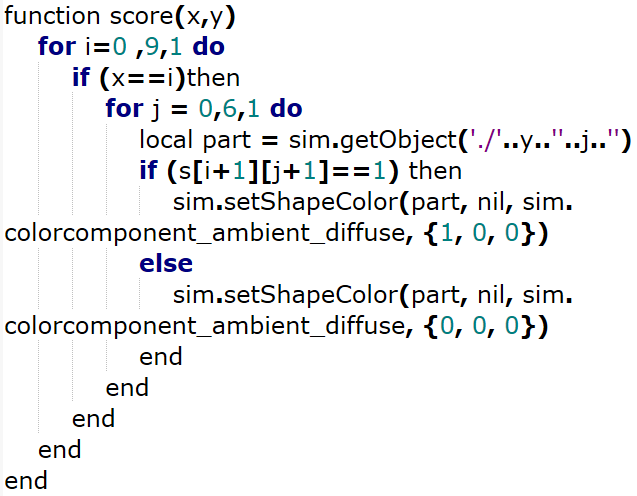
\includegraphics[width=10cm]{47}
\caption{\Large Overview of the resulted Work Orders 結果工單概述}\label{fig.47}
\end{center}
\end{figure}
\fontsize{12}{2.5pt}\selectfont {The problem has been reported by other people (Figure 48) to the Odoo company and is been and hopefully it will be resolved shortly (this is after all a extremelly recent version of the software). That been said, it is a problem even if it is a minor one.
}\\[1pt]

\fontsize{12}{2.5pt}\selectfont {其他人已向 Odoo 公司報告了該問題(圖 48),並希望很快就能得到解決(畢竟這是該軟體的最新版本)。話雖如此,即使這是一個小問題,也是一個問題。}\\[1pt]
\begin{figure}[hbt!]
\begin{center}
\includegraphics[width=10cm]{48}
\caption{\Large mage of Odoo forum question regarding routes  Odoo 論壇法師關於路線的問題}\label{fig.48}
\end{center}
\end{figure}
\fontsize{12}{2.5pt}\selectfont {The manufacturing process was repeated 7 times (Figure 49) to simulate a small batch of prototypes for testing and tolerance checking. It is rare to get a perfect prototype in the first batch, for this reason it was chosen to represent correction through the simulation. In this simulation this problem was a fit problem that resulted in a change of dimension of PROTO Part A.
}\\[1pt]

\fontsize{12}{2.5pt}\selectfont {製造過程重複 7 次(圖 49),以模擬小批量原型進行測試和公差檢查。在第一批中獲得完美原型的情況很少見,因此選擇它來代表透過模擬進行修正。在此模擬中,該問題是一個擬合問題,導致原型 A 部分的尺寸發生變化。}\\[1pt]
\begin{figure}[hbt!]
\begin{center}
\includegraphics[width=10cm]{49}
\caption{\Large Overview of the products after manufacturing 結果工單概述}\label{fig.49}
\end{center}
\end{figure}
\newpage
\fontsize{12}{2.5pt}\selectfont {This give us the opportunity to use ECOs for their actual purpose, stablish and control a change to the product item. The changes to be carried out were on the CAD file regarding the product item. As before we can start the ECO and fill in the description, then the files are uploaded, and the ECO (Figure 50) goes through necessary validation before been made effective.
}\\[1pt]

\fontsize{12}{2.5pt}\selectfont {這使我們有機會將 ECO 用於其實際目的、建立和控制產品項目的變更。要進行的變更是在有關產品項目的 CAD 檔案上進行的。與之前一樣,我們可以啟動 ECO 並填寫描述,然後上傳文件,ECO(圖 50)經過必要的驗證後才會生效。}\\[1pt]
\newpage
\begin{figure}[hbt!]
\begin{center}
\includegraphics[width=10cm]{50}
\caption{\Large Depiction of the validation of the ECO ECO 驗證描述}\label{fig.50}
\end{center}
\end{figure}
\fontsize{12}{2.5pt}\selectfont {The validation procedure basically is set to ask for validation of someone with proper access permissions or specific personnel. In this case, the master account was used to validate and make effective as can be seen from the log in the right side of the image. Once the change
 
is applied you can see that the product item version has been iterated to version 2 as well as a new ECO has been added to the list of ECOs linked to the item (Figure 51).
}\\[1pt]

\fontsize{12}{2.5pt}\selectfont {驗證程序基本上設定為要求具有適當存取權限的人員或特定人員進行驗證。在本例中,主帳戶用於驗證並生效,從圖像右側的日誌可以看出。一旦改變套用後,您可以看到產品項目版本已迭代到版本 2,並且新的 ECO 已新增至連結到該項目的 ECO 清單(圖 51)。}\\[1pt]
\begin{figure}[hbt!]
\begin{center}
\includegraphics[width=10cm]{51}
\caption{\Large Depiction of changes provoked by the ECO to product item  描述 ECO 對產品項目所引起的變化}\label{fig.51}
\end{center}
\end{figure}
\fontsize{12}{2.5pt}\selectfont {That update is followed by another batch of prototypes, the cycle would continue until the prototypes produced satisfy the criteria stablished by the design team. In the case of this simulation it was assumed that one correction was representative enough of this process. This finalizes the development from idea to prototype.
}\\[1pt]

\fontsize{12}{2.5pt}\selectfont {更新之後是另一批原型,循環將繼續,直到生產的原型滿足設計團隊制定的標準。在此模擬的情況下,假設一次校正足以代表該過程。這就完成了從想法到原型的開發。}\\[1pt]










\newpage
\pagenumbering{arabic} %設定頁號阿拉伯數字
\setcounter{page}{1}  %設定頁數
\fontsize{12pt}{2.5pt}\sectionef
\section{Process Plan - Production Test Run - Production製程計劃 - 生產試運轉 - 生產}
\fontsize{12}{2.5pt}\selectfont {Now that the prototype phase is complete the focus will shift to the process. As stablished
before, it was decided to separate the prototype products from the final product item to isolate
the product from the production process during the development. This way many aspects of
development of the product could be evaluated in an ordered manner. Now that the process
is been developed it seems reasonable to create the product items that will represent the final
products since the product of a successful run of the process will be the production ready
samples of it (Figure 52). }\\[1pt]

\fontsize{12}{2.5pt}\selectfont {現在原型階段已經完成,將焦點轉移到流程上。如之前所確定的,決定將原型產品與最終產品項目分開,以在開發過程中將產品與生產過程隔離。這樣可以有序地評估產品開發的許多方面。現在流程已經開發,創建代表最終產品的產品項目似乎是合理的,因為成功運行該流程的產品將是其生產就緒樣本(圖52)。}\\[15pt]

\begin{figure}[hbt!]
\begin{center}
\includegraphics[width=6cm]{52}
\caption{\Large Sectioned diagram regarding Process development 有關流程開發的剖面圖}\label{fig.52}
\end{center}
\end{figure}

\fontsize{12}{2.5pt}\selectfont {Other product items that created were the raw materials for the injection molding (which
are plastic pellets that are fed into the machine to be melted and injected). All that was done
in identical manner to when we create the prototype products with the exception that the
Alpha case (Figure 53) now is marked as sellable and its sale costs are now relevant (Figure
54).  }\\[1pt]

\fontsize{12}{2.5pt}\selectfont {創建的其他產品項目是注塑成型的原材料(其中是送入機器進行熔化和注射的塑膠顆粒)。 一切都已完成與我們創建原型產品時的方式相同,不同之處在於Alpha 案例(圖 53)現在被標記為可銷售,並且其銷售成本現在是相關的(圖54)。}\\[15pt]

\begin{figure}[hbt!]
\begin{center}
\includegraphics[width=6cm]{53}
\caption{\Large Render of how the final product should look like 最終產品的渲染圖}\label{fig.53}
\end{center}
\end{figure}

\begin{figure}[hbt!]
\begin{center}
\includegraphics[width=6cm]{54}
\caption{\Large Product Item of the Alpha Case  Alpha Case 的產品項目}\label{fig.54}
\end{center}
\end{figure}

\fontsize{12}{2.5pt}\selectfont {Once the product items are taken care of, we need to go back to what aspect of the process
will be tracked using Odoo in the context of this simulation. As it was hinted previously when
talking about injection molding the key aspect of change regarding the process are the molds
used by the machines to create the parts. For this simulation it was considered that the mold
development will follow a very similar procedure of the development of the product, this
should be more clear from the following diagram (Figure 55). }\\[1pt]

\fontsize{12}{2.5pt}\selectfont {一旦處理完產品項目,我們需要回到流程的哪個方面將在此模擬的上下文中使用 Odoo 進行追蹤。 正如之前所暗示的那樣談論注塑成型過程中變化的關鍵方面是模具被機器用來製造零件。 對於該模擬,認為模具開發將遵循與產品開發非常相似的程序,這從下圖(圖55)應該比較清楚。}\\[15pt]

\begin{figure}[hbt!]
\begin{center}
\includegraphics[width=6cm]{55}
\caption{\Large Diagram regarding process development for mold 模具製程開發圖}\label{fig.55}
\end{center}
\end{figure}

\fontsize{12}{2.5pt}\selectfont {The production of a prototype mold by 3D printing follows the same standard procedure
for prototyping used for the product. So far, the mold is considered a product like any other,
this reveals another small weakness regarding Odoo ability to represent the totality of the
process. The reader will notice that although the mold is been treated as a product (because
it is been manufactured) it should in fact be considered a tool or piece of equipment as well. }\\[1pt]

\fontsize{12}{2.5pt}\selectfont {透過 3D 列印生產原型模具遵循相同的標準程序用於產品的原型設計。 到目前為止,模具被認為是與其他產品一樣的產品,這揭示了 Odoo 代表整體能力的另一個小弱點過程。 讀者會注意到,雖然模具被視為產品(因為它已經被製造出來了)事實上它也應該被視為一種工具或設備。}\\[15pt]

\fontsize{12}{2.5pt}\selectfont {Although Odoo does makes this distinction between equipment and products, it has no
integration regarding the situations where one is both. In addition, as explained before, there
is no way of uploading CAD files to an equipment item or linking an equipment to a range
of tools. I.e. Odoo does not consider a vertical drill with x number of drill bits to make
different size holes. The closest it can do from the perspective of equipment/maintenance is
consider the vertical drill a workstation and each drill size a separate equipment within the
station with an assigned set up time. This is ok if you ignore that the drill bit is a product. }\\[1pt]

\fontsize{12}{2.5pt}\selectfont {儘管 Odoo 確實對設備和產品進行了區分,但它沒有關於兩者兼而有之的情況的整合。 另外,如同前面所解釋的,還有無法將 CAD 檔案上傳到裝置項目或將裝置連結到範圍的工具。 IE。 Odoo 不考慮使用 x 鑽頭數量的垂直鑽孔機不同尺寸孔。 從設備/維護的角度來看,它能做的最接近的是將立式鑽孔機視為工作站,並將每個尺寸的鑽孔機視為獨立的設備具有指定設定時間的電台。 如果你忽略了鑽頭是一種產品,這也沒關係。}\\[15pt]

\fontsize{12}{2.5pt}\selectfont {All of this is reasonable from the perspective of an ERP system but not ideal from the
perspective of PLM because it shows gaps in between items that should represent the same
thing. In production from the manufacturing application what is set is the work center station
not the equipment (see Figure 41). In the maintenance app there is no connection to the fact
that the tool is a consumable product, you can consider a maintenance schedule and even
make a useful life parameters but because it is an equipment you can’t have reserve tools
like drill bits in inventory like consumables.}\\[1pt]

\fontsize{12}{2.5pt}\selectfont {這一切從ERP系統的角度來看是合理的,但從實際應用角度來看卻不理想。PLM 的視角,因為它顯示了應該代表相同內容的項目之間的差距事物。 在製造應用程式的生產中,設置的是工作中心站不是設備(參見圖 41)。 在維護應用程式中,與事實無關該工具是消耗品,您可以考慮維護計劃,甚至制定使用壽命參數,但因為它是設備,所以不能有備用工具就像庫存中的鑽頭一樣,就像消耗品一樣。}\\[15pt]

\fontsize{12}{2.5pt}\selectfont {The result is that it becomes very difficult to represent testing with a prototype mold. If
you do as the software is designed for you need to create a separate ECO to apply every
operation for each different iteration of the mold development to the necessary BOMs and
make a test run (Figure 56). At this point, considering the maintenance aspect of the mold as
a tool just does not make sense because it would entails filing in metadata in the maintenance
App by hand for every prototype mold iteration all without causing any difference from the
manufacturing perspective. The PROTO mold item ends up been used only for the sake of
tracking material and holding files as the mold is improved. }\\[1pt]

\fontsize{12}{2.5pt}\selectfont {結果是用原型模具來表示測試變得非常困難。 如果您所做的,因為該軟體是為您需要建立一個單獨的 ECO 來應用每個模具開發的每個不同迭代的操作都需要必要的 BOM 和進行測試運行(圖 56)。 此時,考慮到模具的維護面工具沒有意義,因為它需要在維護中歸檔元數據為每個原型模具迭代手動應用程序,不會造成與實際模型的任何差異製造角度。 原型模具專案最終僅用於隨著模具的改進,追蹤材料並保存文件。}\\[15pt]
\newpage
\begin{figure}[hbt!]
\begin{center}
\includegraphics[width=6cm]{56}
\caption{\Large ECO example of update procedure of BOM BOM更新流程ECO範例}\label{fig.56}
\end{center}
\end{figure}

\fontsize{12}{2.5pt}\selectfont {Taking this in consideration, in simulation it will be produced one 3D printed mold for
each part of the alpha case. Then ECOs for the prototype parts of the case will be created to
be applied to the parts BOMs updating the operation from 3D printing to injection molding
test run with prototype molds.}\\[1pt]

\fontsize{12}{2.5pt}\selectfont {考慮到這一點,在模擬中將生產一個 3D 列印模具alpha 案例的每個部分。 然後將創建案例原型部分的 ECO適用於零件 BOM,將操作從 3D 列印更新為射出成型使用原型模具進行試運行。}\\[15pt]

\fontsize{12}{2.5pt}\selectfont {At this point we could differentiate the product prototype from the test run prototype by
making a new prototype product item, however considering our rapidly growing list of
product items (Figure 57) it was concluded that it would be just better for depiction in this
work to modify the previously produced product prototypes (made with 3D printing) and justuse the same items. We can do this because those prototypes have already served their
purpose.  }\\[1pt]

\fontsize{12}{2.5pt}\selectfont {此時,我們可以透過以下方式區分產品原型和試運行原型:製作一個新的原型產品項目,但考慮到我們快速成長的列表產品項目(圖 57)的結論是,在此描述會更好修改先前製作的產品原型(透過 3D 列印製作)並僅使用相同的物品。 我們可以做到這一點,因為這些原型已經投入使用目的。}\\[15pt]
\newpage
\begin{figure}[hbt!]
\begin{center}
\includegraphics[width=6cm]{57}
\caption{\Large Overview of product items at this stage of the simulation 模擬此階段的產品項目概述}\label{fig.57}
\end{center}
\end{figure}

\fontsize{12}{2.5pt}\selectfont {After the mold have been created and the BOMs for the prototypes are updated to include
the injection stations and the proper operations (specifying the use of the molds) the next step
is to do a production test run of prototype. Again that is done by emitting the MO completing
the generated WOs (see Figure 46 and Figure 47 of previous section). }\\[1pt]

\fontsize{12}{2.5pt}\selectfont {創建模具並更新原型的 BOM 後,包括注射站和正確的操作(指定模具的使用)下一步是對原型進行生產測試。 同樣,這是透過發出 MO 完成來完成的生成的 WO(參見上一節的圖 46 和圖 47)。}\\[15pt]

\fontsize{12}{2.5pt}\selectfont {The result of the production is used to check for dimension and fitting, if correction is
needed the ECOs would be emitted again as seen in Figure 56, and a new iteration of
production and testing would be carried out. This process would repeat until the product is
satisfactory enough to justify the production of the CNC machined molds that would be used
in mass production.  }\\[1pt]

\fontsize{12}{2.5pt}\selectfont {生產結果用於檢查尺寸和配合,如果修正的話需要再次發出 ECO,如圖 56 所示,並且新的迭代將進行生產和測試。 這個過程會重複,直到產品被足以證明所使用的 CNC 加工模具的生產是合理的在批量生產中。}\\[15pt]

\fontsize{12}{2.5pt}\selectfont {Since in this simulation it was chosen that the final mold (made of aluminum) would also
be produced in house, this is the next step of development. Procedure is basically the same
as before except that it is needed to create product items for both the raw material (aluminum
block) and the CNC molds prior to their manufacturing. Creating BOMs and uploading
relevant files. }\\[1pt]

\fontsize{12}{2.5pt}\selectfont {由於在此模擬中選擇最終模具(由鋁製成)也將內部生產,這是下一步的開發。 流程基本相同與以前一樣,只是需要為原材料(鋁)創建產品項目塊)和製造前的 CNC 模具。 建立 BOM 並上傳相關文件。}\\[15pt]

\fontsize{12}{2.5pt}\selectfont {Finally, the actual production on the new molds can begin. To represent that a
manufacturing order of 100 Alpha Cases were created. This marks the end of the main path
of development from idea to production (Figure 58).}\\[1pt]

\fontsize{12}{2.5pt}\selectfont {最後,新模具可以開始實際生產。 來表示一個創建了 100 個 Alpha Case 的製造訂單。 這標誌著主路徑的結束從創意到生產的開發過程(圖 58)。}\\[15pt]

\begin{figure}[hbt!]
\begin{center}
\includegraphics[width=6cm]{58}
\caption{\Large Main path of development from idea to production 從創意到生產的主要發展路徑}\label{fig.58}
\end{center}
\end{figure}

\newpage
\pagenumbering{arabic} %設定頁號阿拉伯數字
\setcounter{page}{1}  %設定頁數
\begin{center}
\fontsize{18}{16}\selectfont \textbf{介紹}\\
\end{center}
\fontsize{12pt}{2.5pt}\sectionef
\section{Process upgrade procedure 製程升級流程}
\fontsize{12}{2.5pt}\selectfont {The previous sections were about the procedure that would be necessary to use the Odoo software to track change during the main development of product. As such, most of what was described focused in the use of PLM and the standard procedure of creating and utilizing items like Products, BOMs, ECOs, MOs, WOs and Operations. This section will be different in the sense that now we have a production being carried out and the idea is to test Odoo in its capabilities of performing upgrades (Figure 59 and Figure 60). In other words, performance and feedback of information (and of course MES) becomes the main subject.}\\[1pt]

\fontsize{12}{2.5pt}\selectfont {前面的部分介紹了在產品主要開發過程中使用 Odoo 軟體追蹤變更所需的程序。 因此,所描述的大部分內容都集中在 PLM 的使用以及創建和利用產品、BOM、ECO、MO、WO 和營運等專案的標準程序。 本節將有所不同,因為現在我們正在進行生產,目的是測試 Odoo 執行升級的能力(圖 59 和圖 60)。 換句話說,訊息(當然還有MES)的表現和回饋成為主要課題。}\\[15pt]

\begin{figure}[hbt!]
\begin{center}
\includegraphics[width=15cm]{59}
\caption{\Large Sectioned diagram regarding Process upgrade procedure 有關流程升級程序的剖面圖}\label{fig.59}
\end{center}
\end{figure}

\begin{figure}[hbt!]
\begin{center}
\includegraphics[width=15cm]{60}
\caption{\Large Sectioned diagram regarding Process development 有關流程開發的剖面圖}\label{fig.60}
\end{center}
\end{figure}

\fontsize{12}{2.5pt}\selectfont {Change is always enacted using the ECO functionality even in this case. To remind the reader the situation in which this change will be applied (Figure 61) is the product overview of the relevant product items. Every product item in that list (that is not a raw material) poses at least one BOM and two ECOs already applied to them in order to signify the initial state of every product item (Figure 62). The first ECO of every item affects the product and it holds the initial related files, the second is applied to the BOM of the product in order to hold files related to the initial state of the process as well as record the initial state of the BOM. Without these ECOs (Figure 62), when we ever applied an improvement, the initial state of the product files or BOMs would be lost.}\\[1pt]

\fontsize{12}{2.5pt}\selectfont {即使在這種情況下,也始終使用 ECO 功能來實施變更。 為了提醒讀者將套用此變更的情況(圖 61)是相關產品項目的產品概述。 此清單中的每個產品項目(不是原材料)至少包含一個 BOM 和兩個已應用於它們的 ECO,以表示每個產品項目的初始狀態(圖 62)。 每個專案的第一個 ECO 影響產品並保存初始相關文件,第二個 ECO 應用於產品的 BOM,以便保存與流程初始狀態相關的文件並記錄 BOM 的初始狀態。 如果沒有這些 ECO(圖 62),當我們應用改進時,產品檔案或 BOM 的初始狀態將會遺失。}\\[15pt]

\newpage
\begin{figure}[hbt!]
\begin{center}
\includegraphics[width=15cm]{61}
\caption{\Large Relevant product items overview 相關產品項目概述}\label{fig.61}
\end{center}
\end{figure}
\newpage
\begin{figure}[hbt!]
\begin{center}
\includegraphics[width=15cm]{62}
\caption{\Large Example of ECOs of a product item 產品項目的 ECO 範例}\label{fig.62}
\end{center}
\end{figure}

\fontsize{12}{2.5pt}\selectfont {This time around the production duration and the estimated duration of the process is something that need to be taken in consideration so we can perceive how that applied change on the process affect production. To this end a MO of 50 units of Alpha Case will be created with each operation being estimated to take 30 seconds (15s for parts B/C because there is the need for 2 of them). Meaning that in an ideal situation the total length would be 50 minutes (25 of injection production being done in parallel and 25 for final assembly).In this simulated manufacturing run it was chosen that the injection operations would take slightly more time to complete to be representative of a suboptimal performance. This is been done to see how Odoo reacts and informs in real time the situation in hand.The first phase of the production in the injection process that is carried out in parallel for parts A and B/C on the injection stations 1 and 2. The following (Figure 64) shows how in the beginning of the process the overview of the productions stations indicate with green circles. These circulars signaling in known as Andon and although it is not always considered part of MES it is commonly an integrated feature in many MES systems. After the production process have been carried out with a little delay the circle turned gray and overall efficiency has been marked red on the station tabs (Figure 64).
}\\[1pt]

\fontsize{12}{2.5pt}\selectfont {這次需要考慮生產持續時間和流程的估計持續時間,以便我們能夠了解流程中應用的變更如何影響生產。 為此,將建立 50 個 Alpha Case 單元的 MO,每個操作預計需要 30 秒(B/C 部分需要 15 秒,因為需要其中 2 個)。 這意味著在理想情況下,總長度為 50 分鐘(25 分鐘的注射生產並行完成,25 分鐘用於最終組裝)。在此模擬製造運行中,選擇注射操作需要稍長的時間才能完成,以代表次優性能。 這樣做是為了了解 Odoo 如何反應並即時告知當前情況。注射過程的第一階段生產在註射站 1 和 2 上並行進行 A 和 B/C 部件。下圖(圖 64)顯示了在過程開始時的生產概覽車站以綠色圓圈表示。 這些循環訊號被稱為 Andon,儘管它並不總是被視為 MES 的一部分,但它通常是許多 MES 系統中的整合功能。 生產過程稍有延遲後,圓圈變為灰色,並且整體效率在工作站標籤上標記為紅色(圖 64)。}\\[15pt]

\begin{figure}[hbt!]
\begin{center}
\includegraphics[width=15cm]{63}
\caption{\Large Workcenter overview 1 工作中心概述1}\label{fig.63}
\end{center}
\end{figure}

\begin{figure}[hbt!]
\begin{center}
\includegraphics[width=15cm]{64}
\caption{\Large Workcenter overview 2 工作中心概述2}\label{fig.64}
\end{center}
\end{figure}

\fontsize{12}{2.5pt}\selectfont {The production was carried out twice before any improvement was applied. The first improvement to be carried out were on the production process on the operation and the raw materials used. More specifically, a new operation representative of an equipment upgrades on the injection machines and the replacement of the brand of plastic pellets use in the injection process (Figure 65).
}\\[1pt]

\fontsize{12}{2.5pt}\selectfont {在進行任何改進之前,生產進行了兩次。 首先要進行的改進是生產過程中的操作和所使用的原料。 更具體地說,新的操作代表了注射機的設備升級以及注射過程中使用的塑膠顆粒品牌的更換(圖 65)。}\\[15pt]

\begin{figure}[hbt!]
\begin{center}
\includegraphics[width=15cm]{65}
\caption{\Large ECO applied to BOM ECO應用於BOM}\label{fig.65}
\end{center}
\end{figure}

\fontsize{12}{2.5pt}\selectfont {These upgrades were applied to the BOMs of parts A and B of the Alpha case and production recommenced. After two other MOs producing 50 products each simulating an improvement to the process the following types of data were automatically made available by Odoo (Table 3):}\\[1pt]

\fontsize{12}{2.5pt}\selectfont {這些升級已應用於 Alpha 機箱 A 和 B 部件的 BOM,並重新開始生產。 在另外兩個 MO 生產 50 個產品(每個產品模擬流程改善)後,Odoo 會自動提供以下類型的資料(表 3):}\\[15pt]

\begin{table}[htbp]
    \centering
    \label{tab:example}
    \begin{tabular}{|c|c|c|}
        \hline
        關於WO: & 關於 MO: &整體裝備\\
        \hline
            -持續時間偏差 &-缺貨順序 & -數量\\
       -每單位的持續時間 & -額外開銷& \\
       - 預計持續時間 & -生產數量& \\
        -數量 & -總數量& \\
 - 實際持續時間 &  & \\
    \hline
    \end{tabular}
\end{table}

\fontsize{12}{2.5pt}\selectfont {It should be commented that the data regarding MOs is unfortunately captured in a monthly basis as opposed to the other two categories that process data per order executed. This means that since this simulation is using a trial version of the software that lasts only 14 days the graphical representation of that data offers an unimpressive view of a single point or a single column. In the long run this is a great way to display performance over time but in the case of this simulation not so much (Figure 66).}\\[1pt]

\fontsize{12}{2.5pt}\selectfont {應該指出的是,不幸的是,與 MO 相關的數據是按月捕獲的,而不是按執行訂單處理數據的其他兩個類別。 這意味著,由於該模擬使用的軟體試用版僅持續 14 天,因此該資料的圖形表示提供了單點或單列的不起眼的視圖。 從長遠來看,這是顯示隨時間變化的性能的好方法,但在本次模擬的情況下效果並不好(圖 66)。}\\[15pt]

\begin{figure}[hbt!]
\begin{center}
\includegraphics[width=15cm]{66}
\caption{\Large Total quantity regarding MO MO 總量}\label{fig.66}
\end{center}
\end{figure}

\fontsize{12}{2.5pt}\selectfont {All the data available can be seen in the form of bar charts, line charts or pie charts automatically generated after the time performance is registered (which happens at any moment an action is performed in a work order). Figure 67, Figure 68 and Figure 69 are examples of the results of the 5 production runs:}\\[1pt]

\fontsize{12}{2.5pt}\selectfont {所有可用資料都可以以長條圖、折線圖或圓餅圖的形式查看,這些資料是在註冊時間績效後自動產生的(在工單中執行操作的任何時刻都會發生)。 圖 67、圖 68 和圖 69 是 5 次生產運行的結果範例:}\\[15pt]

\begin{figure}[hbt!]
\begin{center}
\includegraphics[width=15cm]{67}
\caption{\Large Real duration regarding work orders 有關工單的實際持續時間}\label{fig.67}
\end{center}
\end{figure}

\fontsize{12}{2.5pt}\selectfont {Something worth mentioning here is that whenever Odoo mentions quantity or duration it is referring to amount per workorder summed (the system does not care if the operations are being carried in parallel). So, on our simulation, making 50 units using 3 operations that should take 30 seconds each the estimated “duration” to be recorded ideally here is 75 minutes per MO.}\\[1pt]

\fontsize{12}{2.5pt}\selectfont {這裡值得一提的是,每當 Odoo 提到數量或持續時間時,它指的是每個工單的總金額(系統不關心操作是否並行進行)。 因此,在我們的模擬中,使用 3 次操作製造 50 個單元,每個操作應花費 30 秒,理想情況下,此處記錄的估計「持續時間」為每個 MO 75 分鐘。}\\[15pt]

\newpage
\begin{figure}[hbt!]
\begin{center}
\includegraphics[width=15cm]{68}
\caption{\Large Duration variation regarding work orders 有關工單的持續時間變化}\label{fig.68}
\end{center}
\end{figure}

\newpage
\begin{figure}[hbt!]
\begin{center}
\includegraphics[width=15cm]{69}
\caption{\Large Overall equipment effectiveness 整體設備效率}\label{fig.69}
\end{center}
\end{figure}

\fontsize{12}{2.5pt}\selectfont {The astute reader will notice that all the data mentioned so far is derived from the time to completion of the operations been carried out, the related amount to the MO and the workcenter utilized. Even so it is impressive how much information can be drawn especially considering that it is all generated automatically.
}\\[1pt]

\fontsize{12}{2.5pt}\selectfont {精明的讀者會注意到,到目前為止提到的所有數據都是從完成作業的時間、與 MO 和所使用的工作中心相關的數量得出的。 即便如此,可以提取的資訊量仍然令人印象深刻,特別是考慮到這些資訊都是自動產生的。}\\[15pt]







\newpage
\chapter{ODOOS ACOMPLISHMENTS REGARDING PLM AND MES ODOO 在 PLM 的成就製造執行系統} 
\pagenumbering{arabic} %設定頁號阿拉伯數字
\setcounter{page}{72}  %設定頁數

\fontsize{12}{2.5pt}\selectfont {This chapter aims to summarize the strengths and weaknesses of the Odoo software focusing on the questions raised on section 4.2. It will also comment Odoo functionalities or lack thereof noticed throughout the simulation also taking the questions into account.}\\[1pt]

\fontsize{12}{2.5pt}\selectfont {本章旨在總結 Odoo 軟體的優點和缺點重點關注4.2節提出的問題。 它還會評論 Odoo 功能或考慮到問題,整個模擬過程中也注意到缺乏這一點。}\\[15pt]

\section{How does the software deals with items? 軟體如何處理專案?}
\fontsize{12pt}{2.5pt}\selectfont
{Overall, the Odoo software presents the user with a wide variety of digital items that can be used to represent several aspects of
manufacturing as well as other aspects of business.This is mainly due to the way the Odoo ERP functionality uses items to track the pull and push actions throughout its use, that is also how automation is achieved in the software.}\\[1pt]

\fontsize{12pt}{2.5pt}\selectfont 
{總體而言,Odoo 軟體為用戶提供了各種各樣的數位項目,可以可用於表示製造的多個方面以及業務的其他方面。這主要是由於 Odoo ERP 功能使用項目來追蹤拉動和在整個使用過程中推動操作,這也是軟體實現自動化的方式。}\\[1pt]

\section{Are all aspects of the product lifecycle represented? 是否代表了產品生命週期的所有面向?}
\fontsize{12pt}{2.5pt}\selectfont 
{One of the disadvantages of being derived from a ERP system is that it focus on the primary scope of ERP (Figure 2) ,that is,
production and sales. The Items in Odoo reflect that. For instance, the development part of the life cycle during the simulation, although the representation was possible it certainly felt like a stretch of functionalities made for the production phase rather than development is self (Figure 70). When developing prototypes for instance many of the steps like creating an ECO just to carry files in the beginning and going through many steps every time an adjustment in the prototype was made felt too bureaucratic or too much of a workaround..}\\[1pt]

\fontsize{12pt}{2.5pt}\selectfont
{源自 ERP 系統的缺點之一是它專注於ERP的主要範圍(圖2),即生產和銷售。 Odoo 中的項目反映那。 例如,模擬過程中生命週期的開發部分,儘管代表性是可能的,它確實感覺像是為生產階段而不是開發階段是自我的(圖70)。 開發原型時例如,許多步驟,例如建立 ECO 只是為了在開始時攜帶文件,每次原型調整時也感覺要經歷許多步驟官僚主義或太多的解決方法。}\\[1pt]

\begin{figure}[hbt!]
\begin{center}
\includegraphics[width=15cm]{70}
\caption{\Large  Diagram representing Odoo scope of ERP 代表 ERP 的 Odoo 範圍的圖表}\label{fig.70}
\end{center}
\end{figure}

\section{How well are each of those items represented? 這些項目的表現如何?}
\fontsize{12pt}{2.5pt}\selectfont 
{Representation levels of the items vary depending on how the item is used. A good example of that is the material focus of product items. In the sense that everything is considered a product with very little distinction between prototypes or raw materials. The
representation of product items or BOM items is very high with a lot of metadata and useful connections to other items. However, even within the manufacturing application there are some items that lack attention. Operations for instance are items that could benefit greatly from more upload capabilities like 3D printing or CNC files. As automation is becoming more widespread in production it is no longer enough to have only PDF or slide instructions.Additionally, other items do not have the ability of holding files not even with the use ofECOs .}\\[1pt]

\fontsize{12pt}{2.5pt}\selectfont
{項目的表示等級會根據項目的使用方式而改變。 一個好的例如,產品的材質重點。 從某種意義上說,一切都是被認為是原型或原材料之間幾乎沒有區別的產品。 這產品項目或 BOM 項的表示非常高,具有大量元資料且非常有用與其他項目的連接。 然而,即使在製造應用中也存在
一些缺乏關注的項目。 例如,營運是可以受益匪淺的項目來自更多上傳功能,如 3D 列印或 CNC 檔案。 隨著自動化逐漸成為在生產中更加廣泛,僅 PDF 或幻燈片說明已不再足夠。此外,即使使用其他項目,也沒有保存文件的能力生態系統}\\[1pt]

\section{How easy it is to create a brand-new product? 創造一個全新的產品有多容易?}
\fontsize{12pt}{2.5pt}\selectfont 
{Product creation is one of the most straightforward procedures in Odoo, it really comes down to using either the Inventory
application or the Manufacturing application to create a new Product and then fill in its metadata. }\\[1pt]

\fontsize{12pt}{2.5pt}\selectfont
{產品創建是 Odoo 中最簡單的過程之一,它真的來了直至使用庫存應用程式或製造應用程式來創建新產品,然後填寫其元資料。}\\[1pt]

\section{How is the product depicted? 產品是如何描述的?}
\fontsize{12pt}{2.5pt}\selectfont 
{The product depiction is clear and concise, the product item allows for an image to be uploaded to the item and used as an icon. The ERP nature of the product items in Odoo means that the metadata is reasonably bias toward information that is used to manage storage and inventory (Weight, Volume, Quantity etc.) but the item also allows for written description as well as providing links to the BOMs and ECOs related to the product. }\\[1pt]

\fontsize{12pt}{2.5pt}\selectfont
{產品描述清晰簡潔,產品項目允許通過圖像上傳到項目並用作圖標。 Odoo 中產品項目的 ERP 性質意味著元資料合理地偏向用於管理儲存和庫存(重量、體積、數量等),但該物品也允許書面描述以及提供與產品相關的 BOM 和 ECO 的連結。}\\[1pt]

\section{How does the product integrate and reference relevant files? 產品如何整合和引用相關文件?}
\fontsize{12pt}{2.5pt}\selectfont 
{There is surely a reasonable attempt in allowing the most valuable items (Product and BOMs) to be able to manage and reference relevant files. However, Odoo does not implement much more than the bare minimum as far as file management goes. The most it can do is allow for files to be uploaded and download manually. This means that whenever someone makes a change in a file it needs to be manually uploaded in ECO. Integration with most files is inexistent except for operation items because the instruction files can be opened and interacted within Odoo during the production. }\\[1pt]

\fontsize{12pt}{2.5pt}\selectfont
{肯定有合理的嘗試來允許最有價值的物品(產品和BOM)能夠管理和引用相關文件。 然而,Odoo 並沒有實現就文件管理而言,遠遠超出了最低限度。 它最多能做的就是允許手動上傳和下載檔案。 這意味著每當有人對需要手動上傳到 ECO 的檔案進行更改。 與大多數文件集成
由於指令檔可以打開,除操作項外不存在在製作過程中與 Odoo 互動。}\\[1pt]

\section{Does changing one affects the other? 改變一個會影響另一個嗎?}
\fontsize{12pt}{2.5pt}\selectfont 
{It does not, files are mostly dealt by Odoo as paperwork for later reference. Anything added file wise that could entail a change in the product or BOM metadata will require someone to be aware of the change and update the information manually.}\\[1pt]

\fontsize{12pt}{2.5pt}\selectfont
{事實並非如此,文件大多由 Odoo 作為文書處理以供以後參考。 任何事物明智地添加文件可能需要更改產品或 BOM 元數據有人了解更改並手動更新資訊。}\\[1pt]

\section{How easy it is to create a brand-new production process? 創造全新的生產流程談何容易?}
\fontsize{12pt}{2.5pt}\selectfont 
{As mentioned before the item the best represents the process is the bill of materials. This item class requires an existing product to be associated with, other that the BOM is no harder to create than a product item.}\\[1pt]

\fontsize{12pt}{2.5pt}\selectfont
{如前所述,最能代表流程的項目是物料清單。 這項目類別需要與現有產品關聯,除此之外,BOM 並不困難建立一個產品項目。}\\[1pt]

\section{How the process is depicted? 其過程是如何描述的?}
\fontsize{12pt}{2.5pt}\selectfont 
{The process is depicted in the BOM as a list of components (other product items) and operations that are carried out in as specific order to produce a number of end products. This representation seems to sit well with the production procedure. Metadata is kept to a minimum but there is still the capability to offer a text description.}\\[1pt]

\fontsize{12pt}{2.5pt}\selectfont
{此流程在 BOM 中描述為元件清單(其他產品項目)和按特定順序進行的操作,以生產多種最終產品。 這代表性似乎與生產程序吻合。 元資料保存到最低限度,但仍能提供文字描述。}\\[1pt]

\section{How does the process integrate and reference the product itproduces? 流程如何整合並引用產品產生?}
\fontsize{12pt}{2.5pt}\selectfont 
{The integration between the BOM and the product items is by far the most well done in Odoo. Changes made in the BOM affect production and are directly linked to the product.Whenever metadata changes are possible and said aspect is represented in the product itemas well the change of one is inherited by the other.}\\[1pt]

\fontsize{12pt}{2.5pt}\selectfont
{BOM 和產品項目之間的整合是迄今為止做得最好的奧杜。 BOM 中的變更會影響生產並直接與產品相關。每當元資料可能發生變化並且所述方面在產品項中表示時一個人的改變也會被另一個人繼承。}\\[1pt]

\section{Does changing one affects the other? 改變一個會影響另一個嗎?}
\fontsize{12pt}{2.5pt}\selectfont 
{As far as inventory and manufacturing is concerned integration is and referencing is well implemented. Production results flawlessly in the resulting changes in inventory and the navigation path of the GUI is very well optimized. It does not take more than 3 or 4 clicks to get from one product to another or to navigate to other relevant items. }\\[1pt]

\fontsize{12pt}{2.5pt}\selectfont
{就庫存和製造而言,整合和參考都很好實施的。 生產結果完美地體現在庫存和生產的變化上GUI 的導航路徑得到了很好的最佳化。 點擊次數不超過 3 或 4 次從一種產品轉到另一種產品或導航至其他相關項目。}\\[1pt]

\section{How easy is to improve an existing product/ production process? 改善現有產品/生產流程有多容易?}
\fontsize{12pt}{2.5pt}\selectfont 
{As mentioned previously, all improvements in Odoo are performed using engineering change orders. These are applied to product items or bill of materials. Creating ECOs is quite easy and organized, the ECO is an item on itself that symbolizes a signal given to create change, once effective, it symbolizes an increment on the product or process.}\\[1pt]

\fontsize{12pt}{2.5pt}\selectfont
{如前所述,Odoo 中的所有改進都是使用工程來執行的更改訂單。 這些適用於產品項目或物料清單。 創建 ECO 相當重要,ECO 簡單且有條理,它本身就是一個象徵著創造的訊號變革一旦生效,就像徵著產品或流程的增量。}\\[1pt]

\section{How easy it is to update its metadata 更新元數據有多容易}
\fontsize{12pt}{2.5pt}\selectfont 
{It is easy to update any metadata regarding any item in Odoo; however, it is wise to point out that since the ECOs are separate items that are just point by products or BOMs many of the changes are not automatic and require manual intervention. I.e. an ECO will not change the text description of the product for instance. If the new update were to require a change on that description it would require a manual intervention from the user in the product item. Doing that is easy, but it is an extra task that will not be tracked by the ECO.  }\\[1pt]

\fontsize{12pt}{2.5pt}\selectfont
{更新 Odoo 中任何項目的任何元資料都很容易; 然而,明智的做法是指出指出由於 ECO 是單獨的項目,僅按產品或 BOM 點,因此許多更改不是自動的,需要手動幹預。 IE。 ECO 不會改變例如產品的文字描述。 如果新的更新需要更改根據該描述,需要使用者對產品項目進行手動幹預。這樣做很容易,但這是一項額外的任務,ECO 不會追蹤。}\\[1pt]

\section{How easy it is to determine the effects of the change? 確定變革的影響有多容易?}
\fontsize{12pt}{2.5pt}\selectfont 
{Odoo feedback of information is mainly done in a manufacturing order basis. The information available is clear and ECOs do not affect MOs that are already under way so the effects of an applied ECO would not be hard to notice. However, it is good to point out that in the way the performance information is displayed there is no indication of the product revision or the ECO applied. This means that the user would need to first figure when the ECO was applied, then navigate to the equivalent MO in the data to draw its conclusions. Although not a problem for recent changes this does becomes problematic if someone want to analyze effects of old changes.}\\[1pt]

\fontsize{12pt}{2.5pt}\selectfont
{Odoo的資訊回饋主要是在製造訂單的基礎上完成的。 這現有資訊很明確,ECO 不會影響已經在進行的 MO,因此應用 ECO 的效果不難注意到。 不過,值得指出的是性能資訊的顯示方式沒有任何產品的指示修訂或應用 ECO。 這意味著用戶需要先計算應用 ECO,然後導航到資料中的等效 MO 來得出結論。雖然最近的變化不是問題,但如果有人想要的話,這確實會成為問題分析舊變化的影響。}\\[1pt]

\section{How does the software deals with different product revisions? 軟體如何處理不同的產品版本?}
\fontsize{12pt}{2.5pt}\selectfont 
{Version control is something well covered by the 1 to N relation between product/BOM
and linked ECOs. Every product will have a tab containing all the ECOs applied to it in
chronological order effectively working as a timeline representing the item evolution.}\\[1pt]

\fontsize{12pt}{2.5pt}\selectfont
{產品/BOM 之間的 1 對 N 關係很好地涵蓋了版本控制和連結的 ECO。 每個產品都會有一個選項卡,其中包含應用於該產品的所有 ECO時間順序有效地作為代表專案演變的時間軸。}\\[1pt]

\section{How easy is to find data related to product or process? 尋找與產品或流程相關的數據有多容易?}
\fontsize{12pt}{2.5pt}\selectfont 
{Most of the data related to performance regarding production is concentrated under the reporting tab as mentioned in the previous chapter (Figure 71). }\\[1pt]

\fontsize{12pt}{2.5pt}\selectfont
{大多數與生產績效相關的數據都集中在上一章提到的報告標籤(圖 71)。}\\[1pt]

\begin{figure}[hbt!]
\begin{center}
\includegraphics[width=15cm]{71}
\caption{\Large  GUI Options of data reporting 數據報告的 GUI 選項}\label{fig.71}
\end{center}
\end{figure}

\fontsize{12pt}{2.5pt}\selectfont 
{This means that as far as performance is concerned it is quite easy to find the data. The previous chapter will show examples of possible information that are available within those tabs.In addition to using this path the UI of the product item also has a tab that point to the monthly comparison of production volume regarding the product (Figure 72). Which would be more impressive if there was more than one month in the trial version of Odoo.}\\[1pt]

\fontsize{12pt}{2.5pt}\selectfont
{這意味著就效能而言,查找數據非常容易。 上一章將顯示這些標籤中可能提供的資訊的範例。除了使用此路徑之外,產品項目的 UI 還具有一個選項卡,該標籤指向有關產品的每月產量比較(圖 72)。 如果 Odoo 的試用版有超過一個月的時間,那就更令人印象深刻了。}\\[1pt]

\begin{figure}[hbt!]
\begin{center}
\includegraphics[width=15cm]{72}
\caption{\Large  Total quantity regarding MO from product item 產品項目中有關 MO 的總數量}\label{fig.72}
\end{center}
\end{figure}

\section{How easy is find production numbers? 要找出生產編號有多容易?}
\fontsize{12pt}{2.5pt}\selectfont 
{In addition to the previously mentioned ways, Odoo also makes available a unit forecast graph that records the ins and outs of the inventory. This is particularly useful to estimate sales and balance storage with demand (Figure 73). This feature is not mentioned to much in this work because supply and demand is not so much a MES functionality, but it is to useful to have an overview of the production.}\\[1pt]

\fontsize{12pt}{2.5pt}\selectfont
{除了前面提到的方法之外,Odoo 還提供了一個單位預測圖,記錄庫存的來龍去脈。 這對於估計銷售量以及平衡儲存與需求特別有用(圖 73)。 此功能在本工作中並未過多提及,因為供應和需求與其說是 MES 功能,但它對於了解生產情況非常有用。}\\[1pt]

\begin{figure}[hbt!]
\begin{center}
\includegraphics[width=15cm]{73}
\caption{\Large  Unit forecast overview 單位預測概覽}\label{fig.73}
\end{center}
\end{figure}

\section{How does Odoo generate performance data? Odoo 如何產生效能數據?}
\fontsize{12pt}{2.5pt}\selectfont 
{The astute reader will notice that all the data mentioned so far is derived from the time to completion of the operations been carried out, the related amount to the MO and the workcenter utilized. Even so it is impressive how much information can be drawn especially considering that it is all generated automatically.}\\[1pt]

\fontsize{12pt}{2.5pt}\selectfont
{精明的讀者會注意到,到目前為止提到的所有數據都是從完成作業的時間、與 MO 和所使用的工作中心相關的數量得出的。 即便如此,可以提取的資訊量仍然令人印象深刻,特別是考慮到這些資訊都是自動產生的。}\\[1pt]

\section{How does the software present performance change as a result of a upgrade? 升級後軟體的效能有何變化?}
\fontsize{12pt}{2.5pt}\selectfont 
{In order to identify the change, the user must identify the MOs following the change and see the difference based on that. Ideally it would be nice if the graphical information showed the revision of the product, but this is not present as of Odoo V13.}\\[1pt]

\fontsize{12pt}{2.5pt}\selectfont
{為了識別更改,使用者必須識別更改後的 MO,並基於此查看差異。 理想情況下,如果圖形資訊顯示產品的修訂版本就好了,但從 Odoo V13 開始不存在這種情況。}\\[1pt]

\chapter{CONCLUSION 結論} 

\fontsize{12pt}{2.5pt}\selectfont 
{In chapter 2 I referenced a diagram that represents a theoretical ideal of how the integration of PLM with other systems should be (Figure 74). In that diagram the reader can notice that ideally PLM would be the center of the system with other systems (Including ERP) attached to it. Different from said diagram the Odoo software takes ERP as the center with other systems attached to it. This work has shown that it is certainly possible to use Odoo for PLM and MES however it has also shown that the PLM and MES implementation presents some weaknesses.}\\[1pt]

\fontsize{12pt}{2.5pt}\selectfont
{在第 2 章中,我引用了一個圖表,它代表了 PLM 與其他系統整合的理論理想(圖 74)。 在該圖中,讀者可以注意到,理想情況下,PLM 將成為系統的中心,並附上其他系統(包括 ERP)。 與上述圖表不同的是,Odoo 軟體以 ERP 為中心,其他系統依附於此。 這項工作表明,當然可以將 Odoo 用於 PLM 和 MES,但它也表明 PLM 和 MES 的實施存在一些弱點。}\\[1pt]

\begin{figure}[hbt!]
\begin{center}
\includegraphics[width=15cm]{74}
\caption{\Large  Comparison to the left the adapted diagram as theorized by Saaksvuori, A. and Immonen, A. (2008), to the right Odoo take on how systems interact. 與左側 Saaksvuori, A. 和 Immonen, A. (2008) 理論化的改編圖相比,右側 Odoo 展示了系統如何交互作用。}\label{fig.74}
\end{center}
\end{figure}

\fontsize{12pt}{2.5pt}\selectfont 
{The lack of file upload support on things like operation items, work centers or equipment is something of some concern especially considering 3D printing or CNC because access to the CAD files would prove helpful to the operators. Also, there is a gap in between the facets of product and tool when the company is taking upon themselves to develop and produce said tooling (similar situation founded when developing the molds in the simulation).}\\[1pt]

\fontsize{12pt}{2.5pt}\selectfont
{操作項目、工作中心或裝置等缺乏文件上傳支援是一個令人擔憂的問題,特別是考慮到 3D 列印或 CNC,因為存取 CAD 檔案對操作員很有幫助。 此外,當公司自行開發和生產所述工具時,產品和工具之間存在差距(在模擬中開發模具時也會出現類似情況)。}\\[1pt]

\fontsize{12pt}{2.5pt}\selectfont 
{In addition, although MES provide detailed graphical representation regarding the dataset that it has, it is limited to data derived from the time to completion of the operations been carried out. For instance, it would be very valuable if graphical representation regarding quality control was easily available as well.}\\[1pt]

\fontsize{12pt}{2.5pt}\selectfont
{此外,雖然 MES 提供了有關其擁有的資料集的詳細圖形表示,但它僅限於從已執行操作完成的時間得出的資料。 例如,如果品質控制的圖形表示也很容易獲得,那將非常有價值。}\\[1pt]

\fontsize{12pt}{2.5pt}\selectfont 
{All that said, applying ECOs to BOMs in Odoo is a procedure deserving of praise. The ECO holds the information until it is ready to be applied and then it updates the BOM automatically once the ECO is validated by responsible personnel. It might not look like something so important now because this simulation is dealing with very simple products, but it becomes exponentially more important as complexity increases. E.g. A car with thousands of parts and hundreds of nested BOMs would be considered a nightmare to control and keep track of change if a system like this was not present.}\\[1pt]

\fontsize{12pt}{2.5pt}\selectfont
{儘管如此,在 Odoo 中將 ECO 應用到 BOM 是一個值得讚揚的過程。 ECO 會保留資訊直到準備好應用,然後在負責人員驗證 ECO 後自動更新 BOM。 現在它可能看起來不那麼重要,因為這個模擬處理的是非常簡單的產品,但隨著複雜性的增加,它變得更加重要。 例如。 如果沒有這樣的系統,一輛擁有數千個零件和數百個嵌套 BOM 的汽車將被視為控制和追蹤變更的噩夢。}\\[1pt]

\fontsize{12pt}{2.5pt}\selectfont 
{This software is not perfect for PLM or MES implementation, but it does hold value in the sense of availability and integration with other systems. The functionality is there specially regarding product and process and the software has an extremely interesting integration with its natural ERP functionalities. All this makes up for a system that would suit better:}\\[1pt]

\fontsize{12pt}{2.5pt}\selectfont
{該軟體對於 PLM 或 MES 實施來說並不完美,但在可用性和與其他系統的整合方面確實具有價值。 該功能專門針對產品和流程,並且該軟體與其自然的 ERP 功能進行了非常有趣的整合。 所有這些都彌補了一個更適合的系統:}\\[1pt]

\fontsize{12pt}{2.5pt}\selectfont 
{Small business that could use PLM and MES in a smaller scale.
Companies that deal with less manufacturing and more assembly or distribution taking advantage of the All in One nature of the software.}\\[1pt]

\fontsize{12pt}{2.5pt}\selectfont
{可以在較小規模內使用 PLM 和 MES 的小型企業。
利用軟體的多合一特性,處理更少的製造和更多的組裝或分銷的公司。}\\[1pt]

\fontsize{12pt}{2.5pt}\selectfont 
{It is important to mention that the limitations of Odoo are not in the complexity of the product itself but in the complexity of the operations that surround its development. All things considered you could track a large and complex assembly if it includes only simple manufacturing operations or if more complex engineering tasks are done by suppliers. I.e. you could track the assembly of a motorcycle with ease in Odoo, but the PLM features are not polish enough to track the full evolution/development of its powertrain. It is certainly possible to do so but it would take too much time and effort from the engineering team to be considered worth it just for the sake of having an all in one solution with ERP features.}\\[1pt]

\fontsize{12pt}{2.5pt}\selectfont
{值得一提的是,Odoo 的限制不在於產品本身的複雜性,而是圍繞其開發的操作的複雜性。 考慮到所有因素,如果大型且複雜的組裝僅包括簡單的製造操作,或者如果供應商完成了更複雜的工程任務,那麼您可以追蹤大型且複雜的組裝。 IE。 您可以在 Odoo 中輕鬆追蹤摩托車的組裝,但 PLM 功能還不夠完善,無法追蹤其動力系統的完整演變/開發。 這樣做當然是可能的,但僅僅為了擁有一個具有 ERP 功能的一體化解決方案,工程團隊就會花費太多的時間和精力,才被認為是值得的。}\\[1pt]

\newpage
\end{document}